\documentclass[a4paper, 12pt]{article}
\usepackage{cmap}
\usepackage{amssymb}
\usepackage{amsmath}
\usepackage{graphicx}
\usepackage{floatflt}
\usepackage{amsthm}
\usepackage{upgreek}
\usepackage{setspace}
\usepackage[T2A]{fontenc}
\usepackage[utf8]{inputenc}
\usepackage[normalem]{ulem}
\usepackage{arcs}
\usepackage{mathtext} % русские буквы в формулах
\usepackage[left=2cm,right=2cm, top=2cm,bottom=2cm,bindingoffset=0cm]{geometry}
\usepackage[english,russian]{babel}
\usepackage[unicode]{hyperref}
\newenvironment{Proof} % имя окружения
{\par\noindent{$\blacklozenge$}} % команды для \begin
{\hfill$\scriptstyle\boxtimes$}
\newenvironment{example} % имя окружения для примеров
{\par\noindent{\textsc{\textbf{Пример}.}}} % символ рядом с \begin
{\hfill$\scriptstyle\Box$} % символ рядом с \end
\newcommand{\Rm}{\mathbb{R}}
\newcommand{\Cm}{\mathbb{C}}
\newcommand{\Z}{\mathbb{Z}}
\newcommand{\I}{\mathbb{I}}
\newcommand{\N}{\mathbb{N}}
\newcommand{\p}{\prime}
\newcommand{\Ra}{\Rightarrow}
\newcommand{\ra}{\rightarrow}
\newcommand{\FI}{\Phi}
\newcommand{\Sp}{\text{Sp}}
\renewcommand{\leq}{\leqslant}
\renewcommand{\geq}{\geqslant}
\renewcommand{\alpha}{\upalpha}
\renewcommand{\beta}{\upbeta}
\renewcommand{\gamma}{\upgamma}
\renewcommand{\delta}{\updelta}
\renewcommand{\d}{\partial}
\renewcommand{\Re}{\operatorname{Re}}
\renewcommand{\Im}{\operatorname{Im}}
\newcommand{\Ln}{\operatorname{Ln}}
\newcommand{\Arccos}{\operatorname{Arccos}}
\newcommand{\intab}{\int\limits_a^b}
\newcommand{\intl}{\int\limits_l}
\newcommand{\Arcsin}{\operatorname{Arcsin}}
\renewcommand{\varphi}{\upvarphi}
\renewcommand{\tau}{\uptau}
\renewcommand{\rho}{\uprho}
\renewcommand{\lambda}{\uplambda}
\renewcommand{\psi}{\uppsi}
\renewcommand{\xi}{\upxi}
\newcommand{\sumz}{\sum\limits_{n = 0}^\infty }
\newcommand{\sumo}{\sum\limits_{n = 1}^\infty }
\renewcommand{\epsilon}{\upvarepsilon}
\newcommand{\limdef}{\forall \epsilon >0\ \exists \delta (\epsilon) > 0}
\newcommand{\sumrl}{\sum\limits_{n=-\infty}^{+\infty}}
\newcommand\Norm[1]{\left\| #1 \right\|}
\newcommand\ef[1]{e^{i#1}}
\newcommand{\rl}{f(z) = \ldots + c_{-n}(z-z_0)^{-n} + \ldots + c_{-1}(z-z_0)^{-1} + c_0 + c_1(z-z_0) + \ldots + c_n(z-z_0)^n + \ldots}
\newcommand{\resf}{\underset{z = z_0}{\res}f(z)}
\newcommand{\res}{\operatorname{res}}
\newcommand{\resinf}{\underset{z = \infty}{\res}f(z)}
\newcommand{\Arg}{\operatorname{Arg}}
\newtheorem*{theorem}{Теорема}
\newtheorem*{cor}{Следствие}
\newtheorem*{lem}{Лемма}
\title{\vspace{6.5cm}\textbf{\Huge{Теория функции комплексного переменного}}\\Конспект по 2 курсу 
	специальности «прикладная математика»\\(лектор А. А. Леваков)}
\date{}
\begin{document}
	\maketitle
		\newpage
	\tableofcontents{}
	\newpage
	\section{Комплексные числа.}
	$\bullet$ \textit{Под \textbf{множеством комплесных чисел} $\Cm$ понимают множество упорядоченных пар $(a,b)$ вещественных чисел таких, что на этом множестве введены 3 операции}\begin{enumerate}
		\item $(a_1,b_1) = (a_2,b_2) \Longleftrightarrow a_1 = a_2, b_1 = b_2$;
		\item $(a_1,b_1) + (a_2, b_2) = (a_1+a_2, b_1 + b_2)$;
		\item $(a_1, b_1)\cdot (a_2,b_2) = (a_1a_2 - b_1b_2, a_1b_2 + a_2b_1)$;
	\end{enumerate}
Комплексное число обычно обозначается символом $z$.\\\\
\noindent
\parbox[b][3.5cm][t]{10mm}{
	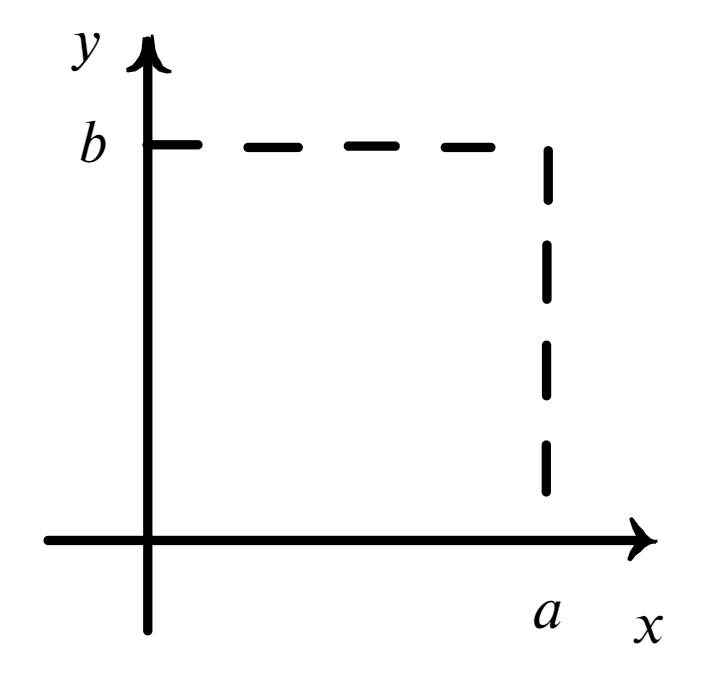
\includegraphics[scale=0.38]{images/001.png}}
\hfill
\parbox[b][2.75cm][t]{115mm}{
Между множеством комплесных чисел и множеством точек ДПСК существует взаимнооднозначное соответствие.\\\\
$\bullet$ \textit{Плоскость с выбранной на ней ДПСК, на которой изображаются комплексные числа, называется \textbf{комплексной плоскостью}.}}\\\\
\noindent
\parbox[b][4cm][t]{110mm}{
Также существует взаимнооднозначное соответствие между множеством комплексных чисел и множеством векторов.\\\\
$\bullet$\textit{ Точки, соответствующие комплексным числам $(a,0)$ лежат на оси $x$. Тогда $(a,0) = a$, а ось $x$ называется \textbf{вещественной}.}}
\hfill
\parbox[b][5cm][t]{55mm}{
	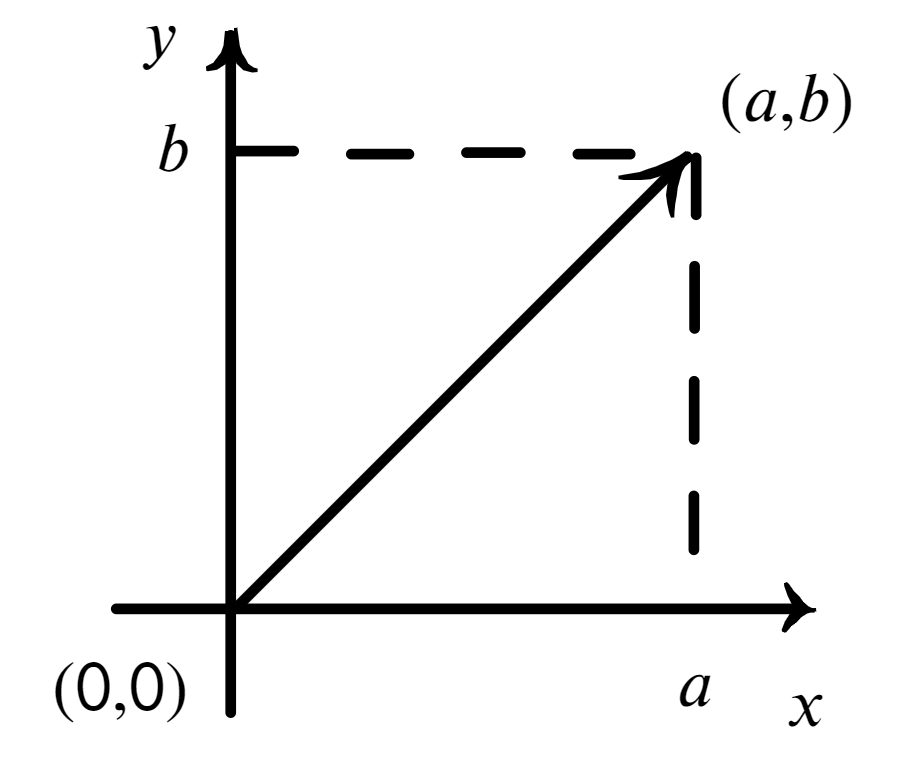
\includegraphics[scale=0.35]{images/002.png}}\\
На множестве комплексных чисел $(0,1)\cdot (0,1) = (-1,0) = -1.$ То есть среди комплексных чисел есть такое число $(0,1) = i$, что $i^2 = 1$.\\\\
$\bullet$ \textit{Точки, соответствующие комплексным числам $(0,b)$ лежат на оси $y$. Тогда $(0,b) = bi$, а ось $y$ называется \textbf{мнимой}}.\\\\
Возьмем произвольное комплексное число $(a,b)$.
$$(a,b) = (a,0) + (0,b) = a+ (b,0)\cdot (0,1) = a+bi.$$
Следовательно, любое комплексное число можно записать в виде $z = a+bi$.\\\\
$\bullet$ \textit{Такая форма записи комплексного числа называется \textbf{алгебраической формой записи}.}\\\\
Как правило, будем записывать комплексные числа в алгебраической форме.\\\\
$\bullet$ \textit{Число $\sqrt{a^2 + b^2} = |z|$ называется \textbf{модулем} комплексного числа.}\\\\
Геометрически это расстояние от начала координат до точки, соответствующей комплексному числу.\\
\noindent
\parbox[b][4.5cm][t]{95mm}{
	$\bullet$ \textit{Угол, который образует вектор к числу $z$ с осью $x$ называется \textbf{аргументом} комплексного числа и обозначается $\varphi = \arg (z)$.}\\\\
	Причем, если вращение вектора от оси $x$ против часовой стрелки, то аргумент считаем положительным. Иначе отрицательным.
	}
\hfill
\parbox[b][5cm][t]{70mm}{
	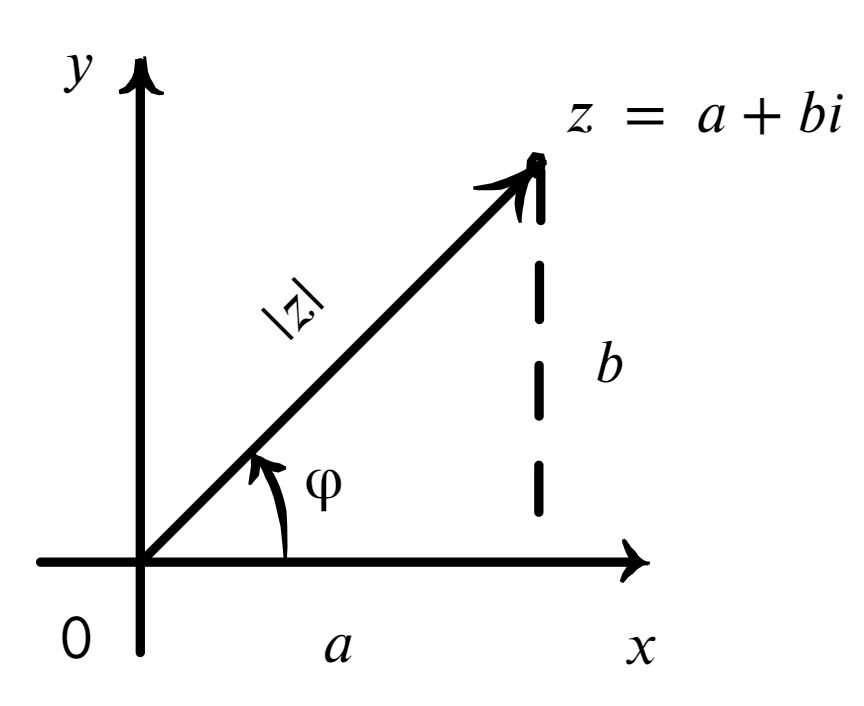
\includegraphics[scale=0.38]{images/003.png}}\\
 Если $\varphi$ --- аргумент, то чиcла $\varphi + 2\pi k$, $k\in \Z$ также являются аргументами (то есть аргумент определен неоднозначно). Обозначаем \begin{itemize}
	\item $\Arg(z) = \varphi + 2\pi k$ --- все значения аргумента;
	\item $\arg (z) = \varphi$ --- одно значение аргумента.
\end{itemize}
Чаще всего $\varphi \in (-\pi; \pi]$. Но иногда удобно считать, что $\varphi \in [0;2\pi)$.\\\\
$\bullet$ \textit{Это фиксированное значение $\arg (z)$ аргумента  называется \textbf{главным значением аргумента} комплексного числа.}\\\\
Таким образом, $a = |z|\cos \varphi$, $b = |z|\sin\varphi$. Тогда можно записать $$z = a + bi = |z|\cdot (\cos \varphi + i\sin\varphi).$$
$\bullet$ \textit{Такая форма записи комплексного числа называется \textbf{тригонометрической формой записи}}.\\\\
Введем функцию $e^{i\varphi}$ опеределенную на множестве $\Rm$ и принимающую значения в множестве $\Cm$ по формуле $$e^{i\varphi} = \cos\varphi + i\sin\varphi.$$
Используя эту функцию, можем записать комплексное число в виде $$z = a+bi = |z|\cdot e^{i\varphi}.$$
$\bullet$ \textit{Такая форма записи комплексного числа называется \textbf{экспоненциальной формой записи}}.\\\\
Покажем, что функция $e^{i\varphi}$ обладает свойствами экспоненты:
\begin{enumerate}
	\item $\ef{\varphi_1}\cdot \ef{\varphi_2} = \ef{(\varphi_1 + \varphi_2)}$.
	\begin{Proof}
		\begin{multline*}
			\ef{\varphi_1}\cdot \ef{\varphi_2} = (\cos\varphi_1, \sin\varphi_1)\cdot (\cos\varphi_2, \sin\varphi_2) =\\= (\cos\varphi_1\cos\varphi_2-\sin\varphi_1\sin\varphi_2,\ \cos\varphi_1\sin\varphi_2 + \sin\varphi_1\cos\varphi_2)=\\=(\cos(\varphi_1 + \varphi_2),\ \sin(\varphi_1 + \varphi_2)) = \ef{(\varphi_1 + \varphi_2)}.
		\end{multline*}
	\end{Proof}
\item $\dfrac{\ef{\varphi_1}}{\ef{\varphi_2}} = \ef{(\varphi_1 - \varphi_2)}.$
\item $(\ef{\varphi})^n = \ef{n\varphi}$, $n\in \N$.
\end{enumerate}
\noindent
\parbox[b][4cm][t]{90mm}{
	Возьмем комплексную плоскость и обозначим на ней 2 комплексных числа и соответствующие им радиус-векторы. Построим параллелограмм на этих векторах и возьмем его диагональ. Комплексное число, соответствующее этой диагонали, имеет вид $z_3 = (a_1 + a_2, b_1 + b_2)$, то есть является суммой комплексных чисел $z_1$ и $z_2$.
	}
\hfill
\parbox[b][5cm][t]{70mm}{
	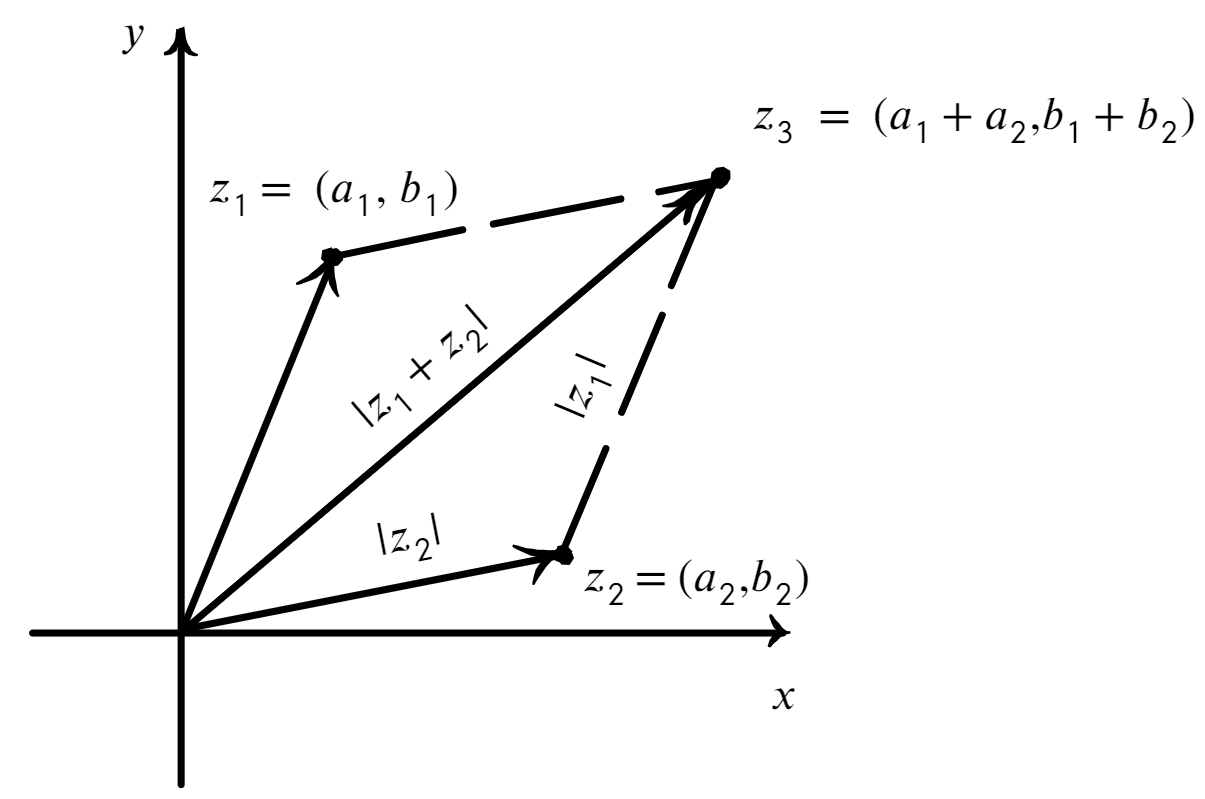
\includegraphics[scale=0.36]{images/004.png}}\\\\
Разность комплексных чисел $z_1-z_2 = z_1 + (-z_2)$ определяется вектором, который является второй диагональю параллеограмма построенного на векторах $z_1$ и $z_2$.
$$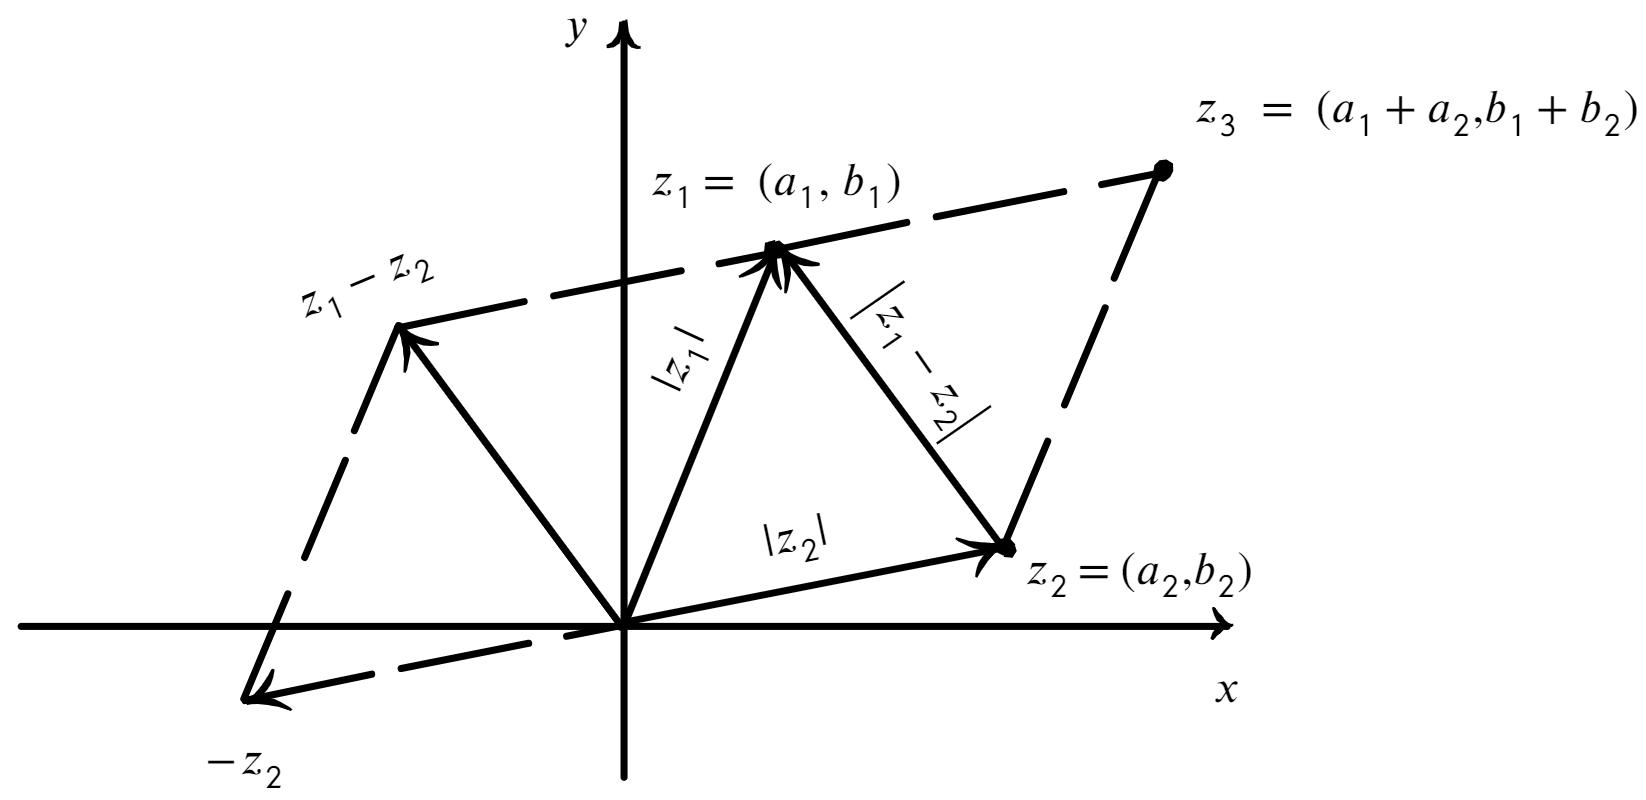
\includegraphics[scale=0.5]{images/005.png}$$
Из графиков следует свойство
$$\big||z_1|-|z_2|\big|\leqslant |z_1 + z_2|\leqslant |z_1| + |z_2|.$$
Из свойств комплексных чисел\\\\
$z_1\cdot z_2 = |z_1|\cdot \ef{\varphi_1}\cdot |z_2|\cdot \ef{\varphi_2} = |z_1|\cdot |z_2| \cdot \ef{(\varphi_1 + \varphi_2)}.$\\\\
$\dfrac{z_1}{z_2} = \dfrac{|z_1|\cdot \ef{\varphi_1}}{|z_2|\cdot \ef{\varphi_2}} = \dfrac{|z_1|}{|z_2|}\cdot \ef{(\varphi_1 - \varphi_2)}.$\\\\
Отсюда вытекает, что
\begin{enumerate}
	\item $|z_1\cdot z_2| = |z_1|\cdot |z_2|$,\quad $\arg(z_1\cdot z_2) = \arg (z_1) + \arg (z_2)$.
	\item $\Big|\dfrac{z_1}{z_2}\Big|=\dfrac{|z_1|}{|z_2|}$, \quad $\arg\Big(\dfrac{z_1}{z_2}\Big) = \arg(z_1) - \arg(z_2)$.
 \end{enumerate}
$\bullet$ \textit{Если число $z = a+bi$ --- комплексное число, то число $\overline{z} = a - bi$ называется \textbf{сопряженным} к комплексному числу $z$.}\\\\
Тогда $z\cdot \overline{z} = a^2 + b^2 = |z|^2.$ Из свойств множества комплексных чисел $$z_1=z_2 \Longleftrightarrow a_1 = a_2,\ b_1 = b_2.$$
В экспоненциальной форме
$$|z_1|\cdot\ef{\varphi_1} = |z_2|\cdot\ef{\varphi_2}\Longleftrightarrow |z_1| = |z_2|,\ \arg(z_1) = \arg(z_2) + 2\pi k,\ k\in \Z.$$
$\bullet$ \textit{\textbf{Корнем n-ой степени} комплексного числа $z$ называется такое число $\upzeta$, что $\upzeta ^ n = z$. Обозначение: $\sqrt[n]{z}$.}\\\\
Пусть $z = |z|\cdot \ef{\varphi}$, $\upzeta = |\upzeta|\cdot \ef{\varphi_1}$. Тогда $$(|\upzeta|\cdot \ef{\varphi_1})^n = |z|\cdot  \ef{\varphi}.$$
$$|\upzeta|^n\cdot\ef{n\varphi_1} = |z|\cdot \ef{\varphi}.$$
Тогда получаем
	\begin{align*}
		|\upzeta|^n = |z| &\Rightarrow |\upzeta| = |z|^{\frac1n}.\\
		n\varphi_1 = \varphi + 2\pi k,\ k \in \Z &\Rightarrow \varphi_1 = \dfrac{\varphi + 2\pi k}{n}.
	\end{align*}
Значит $$\upzeta = |z|^{\frac{1}{n}}\cdot \ef{\frac{\varphi + 2\pi k}{n}}.$$
\noindent
\parbox[b][8.5cm][t]{10mm}{
	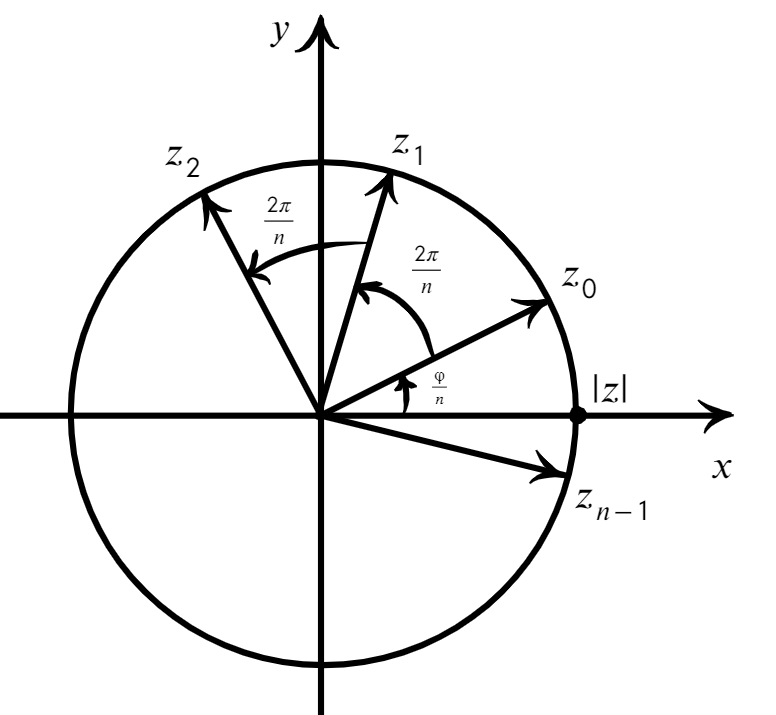
\includegraphics[scale=0.6]{images/006.png}}
\hfill
\parbox[b][6.5cm][t]{65mm}{
	При $k = 0$ получаем $z_0$,\\\\ $k=1\to z_1$,\\\\ $k=2\to z_2$,\\\ $\ldots$,\\\\ $k=n-1\to z_{n-1}$,\\\\ $k = n\to z_0$. }\\
Следовательно, корень $n$-ой степени из любого ненулевого комплексного числа имеет ровно $n$ различных значений. То есть $\sqrt[n]{z} = \upzeta_k$ и $$\upzeta_k = |z|^{\frac1n}\cdot \ef{\frac{(\arg z + 2\pi k)}{n}},\quad k = 0,1,\ldots,n-1.$$
\section{Комплексные функции.}
Пусть $D\subseteq \Rm$, $f:D\to\Cm$.\\\\
$\bullet$ \textit{Функция $w=f(t)$, $t\in D\in\Rm$ называется \textbf{комплекснозначной} функцией.}\\\\
Запишем в алгебраической форме:
$$w=u(t)+i\cdot v(t),\quad \Re (w) = u(t)\in\Rm,\ \Im (w) = v(t)\in\Rm.$$
Производная и интеграл для таких функций определяются аналогично вещественным функциям:
$$w^\p(t) = u^\p(t) + i\cdot v^\p(t).$$
$$\int\limits_{a}^bw(t)dt = \int\limits_{a}^bu(t)dt + i\cdot \int\limits_{a}^bv(t)dt.$$
Рассмотрим функцию $w = e^{it}$, $t\in[0;2\pi)$. Ее можно представить как $e^{it} = \cos t + i\cdot \sin t.$ Тогда производная от этой функции равна $$(e^{it})^\p = -\sin t + i\cdot \cos t = i\cdot (\cos t + i\cdot \sin t) = ie^{it}.$$
Пусть $f : D\to \Cm$, $D\in \Cm$.\\\\
$\bullet$\textit{ Функция $w = f(z)$, $z\in D\in\Cm$ называется \textbf{комплексной функцией}.}\\\\
Это же определение можно сформулировать иначе.\\\\
$\bullet$ \textit{Пусть заданы множества $D\in \Cm$ и $L\in\Cm$ и правило $D\overset{f}{\to}L$, которое каждому значению $z\in D$ ставит в соответствие одно или несколько значений $w \in L$. Это мы и будем понимать под \textbf{комплексной функцией}.}.\\\\
Функцию, ставящую в соответствие одно значение, будем называть \textbf{однозначной}. Аналогично, если два значения, то \textbf{двузначной}. Если неизвестно сколько значений, то \textbf{многозначной}.\\\\
Например, графически двузначная функция будет изображаться таким образом
$$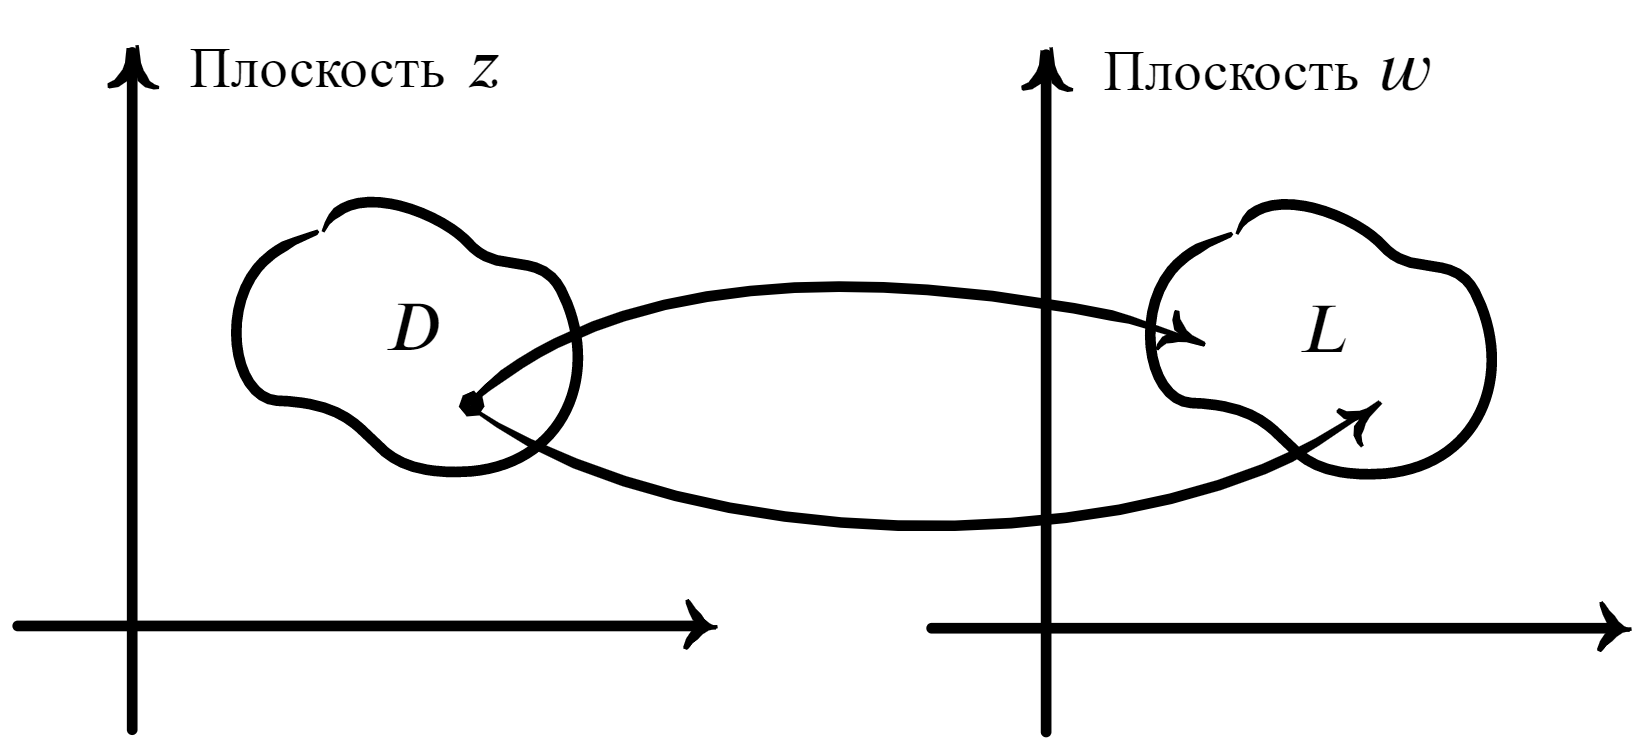
\includegraphics[scale=0.4]{images/007.png}$$
Рассмотрим примеры комлексных функций:\begin{enumerate}
	\item $w = az + b$, $a,b\in \Cm$ --- \textit{\textbf{линейная функция}};
	\item $w = az^2 + bz + c$, $a,b,c\in\Cm$ --- \textbf{\textit{квадратичная функция}};
	\item $w = a_nz^n + a_{n-1}z^{n-1} + \ldots + a_1z + a_0$, $\forall a_i \in \Cm, n\in \N$ --- \textbf{\textit{полином n-ой степени}};\\\\
	Каждый полином $n$-ой степени имеет ровно $n$ корней с учетом кратности.
	\item $w = \sqrt{z}$;\\\\
	Решением этой функции является множество таких $\zeta ^2 = z$, где $$\zeta = |z|^\frac12\cdot\ef{\frac{\arg z + 2\pi k}{2}},\quad k = 0,1.$$
	Тогда $\zeta_1 = |z|^\frac12\cdot\ef{\frac{\arg z}{2}}$, $\zeta_2 = -|z|^\frac12\cdot\ef{\frac{\arg z}{2}}$. Следовательно, $w = \sqrt{z}$ --- двузначная функция.\\\\
	Графически это можно изобразить как $$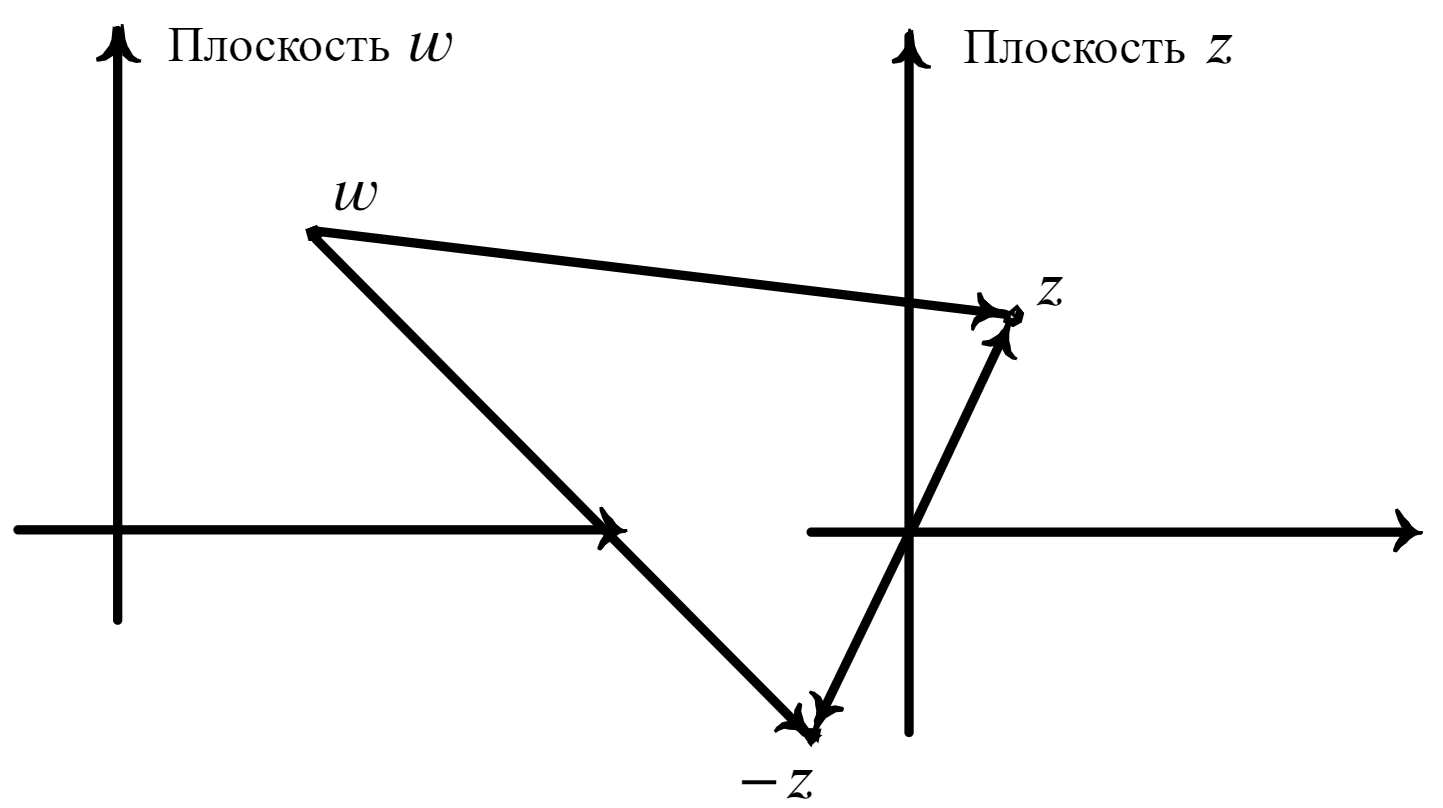
\includegraphics[scale=0.4]{images/008.png}$$
	Функции $w_1 = |z|^\frac12\cdot\ef{\frac{\arg z}{2}}$, $w_2 = -|z|^\frac12\cdot\ef{\frac{\arg z}{2}}$ являются однозначными. Их также называют \textbf{ветвями} двузначной функции $w = \sqrt{z}$.
	\item $w = e^z$ --- \textbf{\textit{комплексная экспонента}};
	$$e^z = e^{x + iy} = e^x(\cos y + i\cdot \sin y) = e^x\cos y + i\cdot e^x \sin y,$$
	то есть $\Re (e^z) = e^x\cos y$, $\Im(e^x) = e^x\sin y$. Если $z = x$, $e^z = e^x$.\\\\
	Рассмотрим уравнение $w_0 = e^z$, $w_0 \ne 0$. 
	\begin{center}
		$\begin{matrix}
			w_0 = |w_0|\cdot e^{i\arg w_0},\\
			e^z = e^x\cdot e^{iy} = e^x \cdot \ef{\arg z};
		\end{matrix}\quad \Longrightarrow\quad  \begin{matrix}
		|w_0|=e^x,\\
		y = \arg z + 2\pi k,\ k\in \Z.
	\end{matrix}$
	\end{center}
Отсюда $x = \ln|w_0|$, $y = \arg z + 2\pi k$, $k\in\Z$. Тогда множество решений уравнения $w_0 = e^z$ имеет вид $$z = \ln |w_0|+i\cdot (\arg z +2\pi k).$$
\item $w = \Ln z = \ln|z| + i\cdot (\arg z + 2\pi k)$, $k\in \Z$ --- \textbf{\textit{комплексный логарифм}};\\\\
Если $z = x > 0$, то при $k = 0$ получим $\ln z = \ln |z| + i\arg z$ --- главное значение (ветвь) $\Ln z$. Эта функция совпадает с вещественной $\ln x$.\\\\
Из двух предудыщих рассмотренных функций вытекает, что во множестве комплексных чисел уравнение $e^z = -1$ имеет множество решений $\Ln(-1) = i\cdot (\pi+ 2\pi k)$, $k\in \Z$.
\item $w = z^\alpha$, $\alpha \in \Cm$ --- \textbf{\textit{степенная функция с любым показателем}};\\\\
Причем $z ^\alpha = e^{\alpha \Ln z}$ при $z \ne 0$.
\item $w = \sin z$, $w = \cos z$ --- \textbf{\textit{комплексные синус и косинус}} соответственно;
$$\sin z = \dfrac{e^{iz} - e^{-iz}}{2i},\quad \cos z = \dfrac{e^{iz} + e^{-iz}}{2}.$$
Проверим, что при $z = x$ получим $\sin z = \sin x$:
$$\sin z = \dfrac{e^{ix} - e^{-ix}}{2i}=\dfrac{\cos x + i\sin x - \cos x + i\sin x}{2i} = \sin x.$$
Комплексные синус и косинус являются $2\pi$-периодическими функциями.\\\\
Все формулы для вещественных синуса и косинуса выполняются и для комплексных. Например, $$\cos^2 z + \sin^2z = \Big(\dfrac{e^{iz} + e^{-iz}}{2}\Big)^2 + \Big(\dfrac{e^{iz} - e^{-iz}}{2i}\Big)^2 = \dfrac{e^{2iz} + e^{-2iz} + 2}{4} + \dfrac{e^{2iz} + e^{-2iz} -2}{-4} = 1.$$
Аналогично доказываются 
\begin{center}
	$\cos ^2z -\sin^2z = \cos 2z,\quad 2\sin z\cos z = \sin2z,\quad \sin(z_1 + z_2) = \sin z_1 \cos z_2 + \sin z_2 \cos z_1$ и так далее.
\end{center}
\end{enumerate}
\begin{example}
	Найдем, чему равно $z$ в уравнении $\cos z = A$.\\\\
	$$\cos z = \dfrac{e^{iz} + e^{-iz}}{2} = [e^{iz} = t] = \dfrac{t + \frac{1}{t}}{2} = A\quad\Rightarrow\quad t^2 - 2At + 1 = 0.$$
	Отсюда $$t = \dfrac{2A + \sqrt{4A^2 -4}}{2} = A + \sqrt{A^2 - 1}.$$
	Тогда $$e^{iz} = A + \sqrt{A^2 - 1}.$$
	Следовательно, $$iz = \Ln (A + \sqrt{A^2 - 1})\quad \Rightarrow\quad z = -i\Ln(A + \sqrt{A^2 - 1}).$$
\end{example}\\
Функция \begin{center}
	$w = -i\cdot\Ln(z + \sqrt{z^2 - 1}) = \Arccos z$ --- \textbf{комплексный арккосинус}.
\end{center} Аналогично можно вывести функцию \begin{center}
	$w = -i\cdot\Ln(iz + \sqrt{1 - z^2}) = \Arcsin z$ --- \textbf{комплексный арксинус}.
\end{center}
\section{Предел функции комплексного переменного. Непрерывные функции комплексного переменного.}
$\bullet$ \textit{Последовательность $(z_n)$, где все члены $z_n \in \Cm$, называется \textbf{комплексной последовательностью}.}\\\\
$\bullet$ \textit{Число $a\in \Cm$ называется \textbf{пределом последовательности $(z_n)$}, если} $$\limdef : \forall n \geqslant \delta (\epsilon) \Rightarrow |z_n - a | \leq \epsilon.$$
\noindent
\parbox[b][4.5cm][t]{10mm}{
	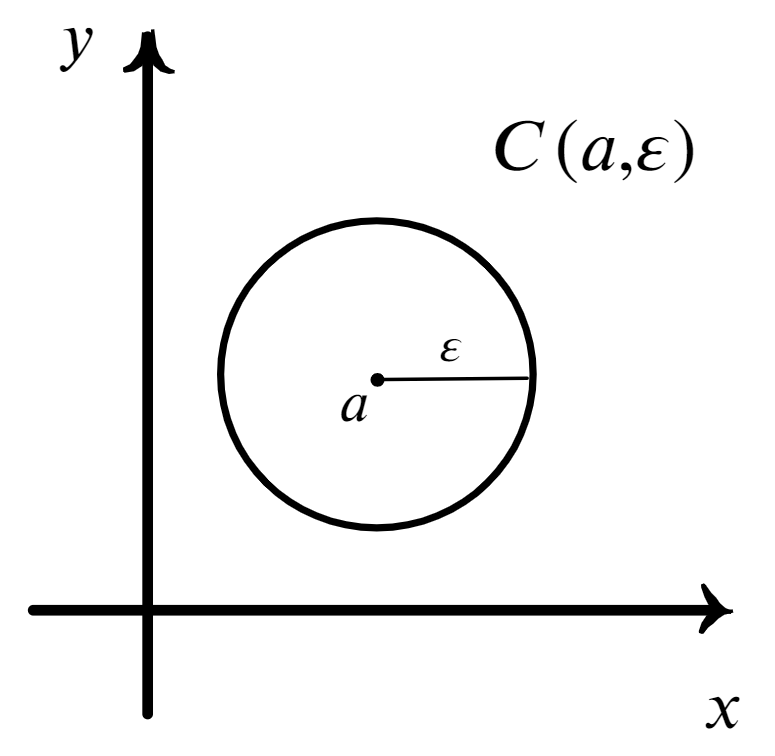
\includegraphics[scale=0.4]{images/009.png}}
\hfill
\parbox[b][4cm][t]{110mm}{Геометрически это множество точек плоскости таких, что $|z-a| = \epsilon$ (расстояние от точки $z$ до точки $a$), то есть это окружность радиуса $\epsilon$ с центром с точке $a$. Обозначается $C(a,\epsilon)$.\\\\Если $|z-a|\leqslant \epsilon$, то это круг с границей радиуса $\epsilon$ с центром с точке $a$. Обозначается $\overline{B}(a,\epsilon)$.\\\\
	Если $|z-a|< \epsilon$, то это круг без границы радиуса $\epsilon$ с центром с точке $a$. Обозначается ${B}(a,\epsilon)$.}\\\\
\begin{center}
	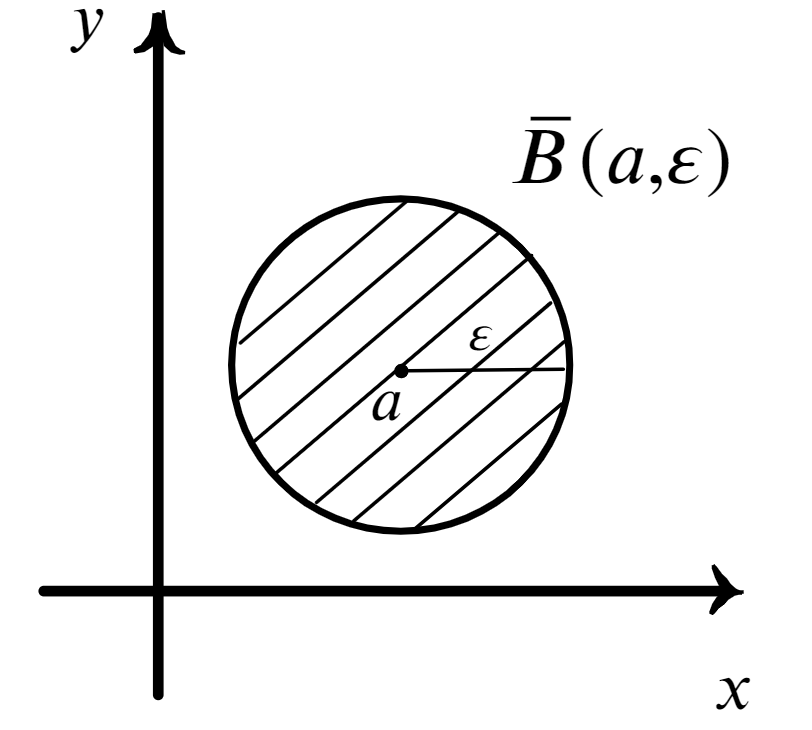
\includegraphics[scale=0.4]{images/010.png}\qquad\qquad\qquad\qquad
	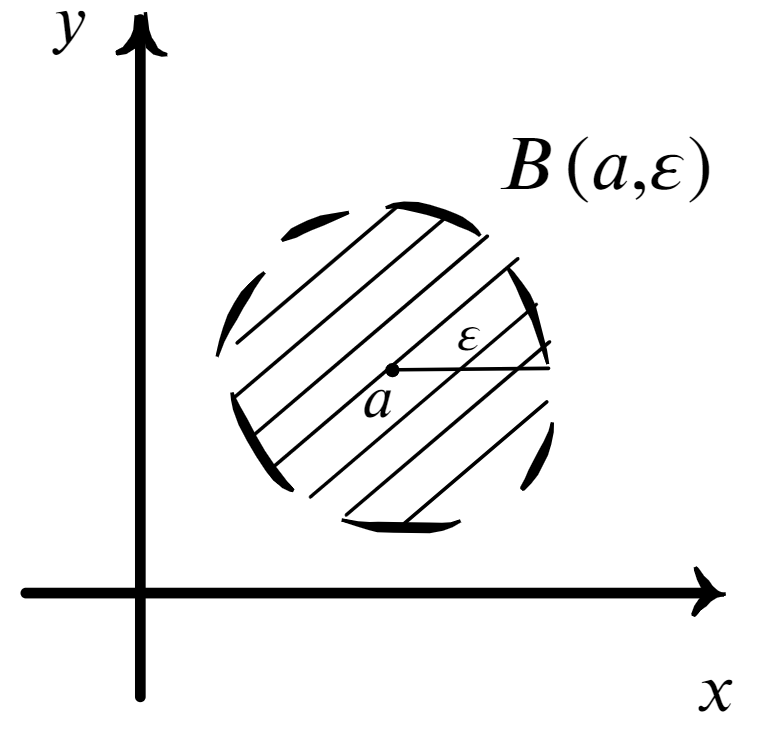
\includegraphics[scale=0.4]{images/011.png}
\end{center}
\noindent
\parbox[b][4.5cm][t]{95mm}{
	Говорят, $B(a,\epsilon)$ --- $\epsilon$-окрестность точки $a$. $\overline{B}(a,\epsilon)$ --- замкнутая $\epsilon$-окрестность точки $a$.\\\\
	Таким образом, число $a\in \Cm$ --- предел последовательности, если $\limdef$ такое, что все члены последовательности $z_n$ с номерами $\geqslant$ чем $\delta (\epsilon)$ лежат в замкнутой $\epsilon$-окрестности числа $a$.\\\\
}
\hfill
\parbox[b][4.5cm][t]{70mm}{
	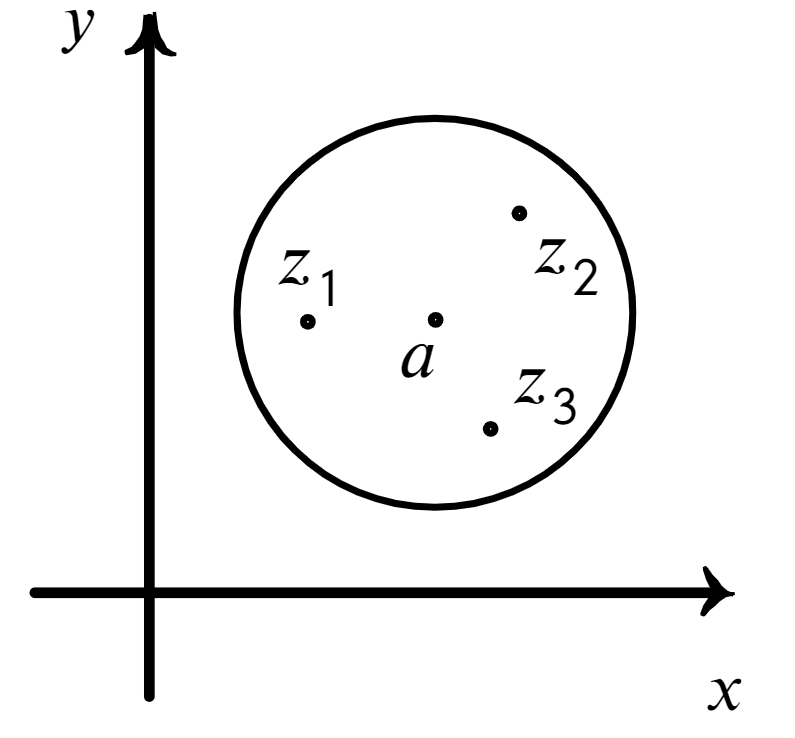
\includegraphics[scale=0.35]{images/012.png}}\\
Говорят, что $(z_n)\underset{n\to\infty}{\longrightarrow} \infty$, если $$\limdef:\forall n \geqslant \delta (\epsilon)\Rightarrow |z_n|\geqslant\epsilon,$$
то есть если $\limdef$ такое, что все члены последовательности $z$ лежат вне $\epsilon$-окрестности числа $a$, или $z_n \not \in B(a,\epsilon)$.\\\\
\noindent
\parbox[b][4.5cm][t]{10mm}{
	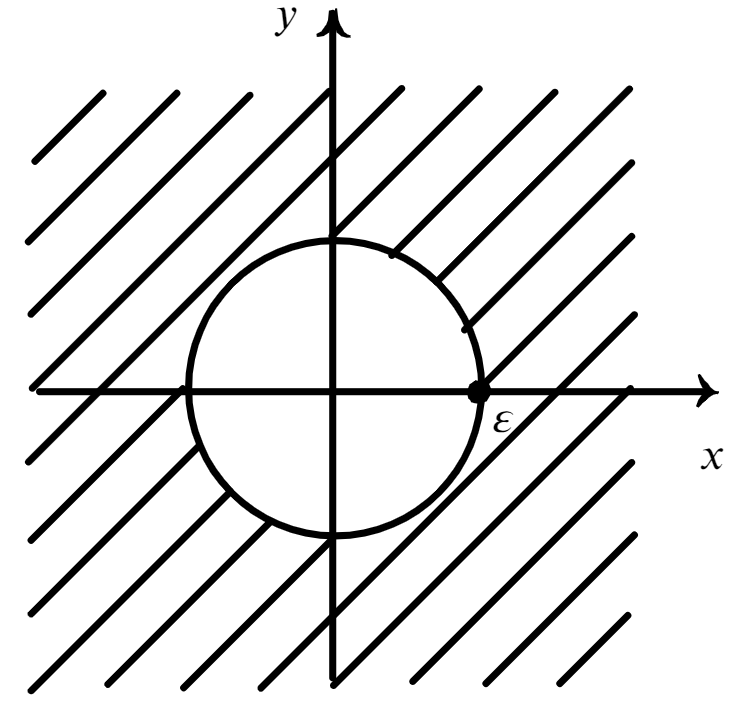
\includegraphics[scale=0.4]{images/014.png}}
\hfill
\parbox[b][4.5cm][t]{110mm}{Дополним множество комплексных чисел $\Cm$ еще одним числом $z = \infty$.\\\\
	$\bullet$ \textit{Множество комплексных чисел, дополненных числом $z = \infty$, называется \textbf{расширенным множеством комплексных чисел}.}\\\\
	Множество таких $z$, что $|z|>\epsilon$, изображается графически (рис. слева)}\\\\
и называется \textbf{окрестностью бесконечности}.\\\\
$\bullet$ \textit{Комлексная плоскость, дополненная точкой $z = \infty$, называется \textbf{расширенной комплексной плоскостью}.}\\\\
Рассмотрим $(z_n)$, где все члены записываются в алгебраической форме: $z_n = x_n + i\cdot y_n$, $x_n,y_n \in \Rm$.
\begin{theorem}
	$z_n \underset{n\to\infty}{\longrightarrow} a = a_1 + i\cdot a_2 \Longleftrightarrow x_n \underset{n\to\infty}{\longrightarrow} a_1,\ y_n \underset{n\to\infty}{\longrightarrow}a_2$.
\end{theorem}
\begin{Proof}
	$\Rightarrow)$ $z_n \underset{n\to\infty}{\longrightarrow} a$, это значит, что $$\limdef : \forall n \geqslant \delta (\epsilon)\Rightarrow |z_n - a| \leqslant \epsilon.$$
	Так как\\
	\noindent
	\parbox[b][4.5cm][t]{10mm}{
		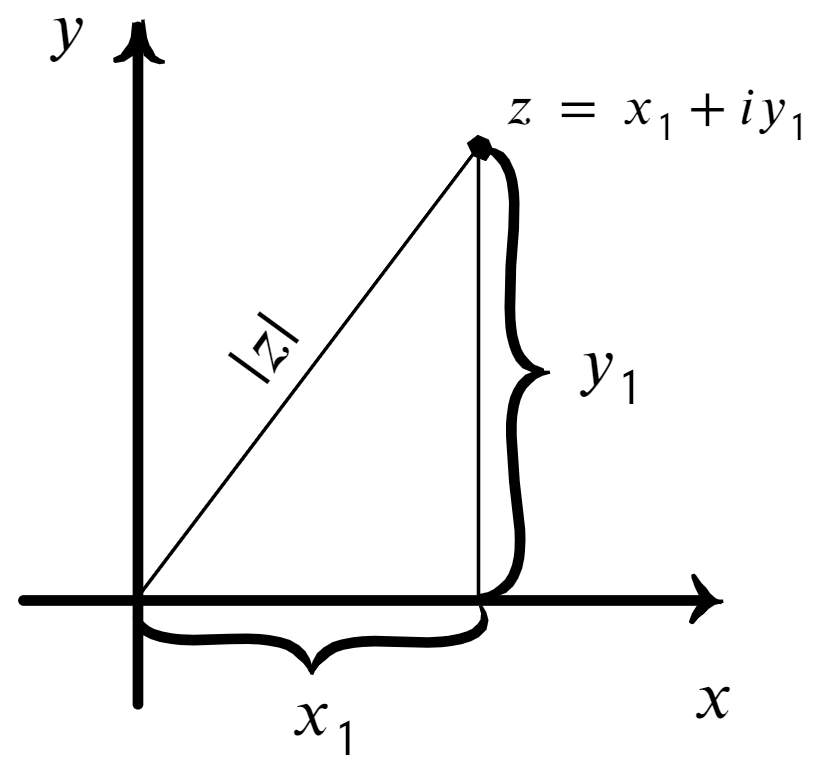
\includegraphics[scale=0.35]{images/015.png}}
	\hfill
	\parbox[b][4cm][t]{100mm}{	то есть $|z| > y$, $|z|>x$, то $$|x_n - a_1|\leqslant |z_n - a|\leqslant \epsilon,$$
		$$|y_n - a_2|\leqslant |z_n - a|\leqslant \epsilon.$$
		Это означает, что $\begin{matrix}
			x_n\underset{n\to\infty}{\longrightarrow}a_1\\
			y_n\underset{n\to\infty}{\longrightarrow}a_2
		\end{matrix}$.
		}\\\\
	$\Leftarrow)$ $\begin{matrix}
		x_n\underset{n\to\infty}{\longrightarrow}a_1\\
		y_n\underset{n\to\infty}{\longrightarrow}a_2
	\end{matrix}$, это значит, что $$\limdef : \forall n \geqslant \delta_1 (\epsilon)\Rightarrow |x_n - a_1| \leqslant \epsilon,$$
$$\limdef : \forall n \geqslant \delta_2 (\epsilon)\Rightarrow |y_n - a_2| \leqslant \epsilon.$$
Тогда $$|z_n - a| = \sqrt{(x_n - a_1)^2 + (y_n-a_2)^2}\leqslant \sqrt{2}\epsilon,\quad \forall n \geqslant \max\{\delta _1(\epsilon), \delta_2(\epsilon)\},$$
а это и есть $z_n \underset{n\to\infty}{\longrightarrow}a$ по $M$-лемме для последовательностей.
\end{Proof}\\\\
\textbf{Замечание.} \textit{Если члены последовательности записаны в экспоненциальной форме $z_n = \rho_n e^{i\varphi_n}$, то $z_n \underset{n\to\infty}{\longrightarrow} a = \rho e^{i\varphi_0} \not\Leftrightarrow \rho_n \underset{n\to\infty}{\longrightarrow}\rho$, $\varphi_n \underset{n\to\infty}{\longrightarrow}\varphi_0$, так как $\varphi_n$ определено неоднозначно. Выполняется только} $$\rho_n \underset{n\to\infty}{\longrightarrow}\rho,\ \varphi_n \underset{n\to\infty}{\longrightarrow}\varphi_0 \Longrightarrow z_n \underset{n\to\infty}{\longrightarrow} a = \rho e^{i\varphi_0}.$$
Рассмотрим функцию $w = f(z)$, $z\in D\subseteq\Cm$. Любую функцию можно записать как $$w = f(z) = f(x+i\cdot y) = u(x,y) + i\cdot v(x,y),\quad u(x,y)\in \Re(f(z)), v(x,y)\in \Im(f(z)),$$ где $u(x,y)$ и $v(x,y)$ --- вещественные Ф2П.\\\\
Пусть точка $z_0$ --- вутрення точка множества $D$.\\\\
$\bullet$ \textit{Множество $D\backslash\{z_0\}$ называется \textbf{проколотой окрестностью} точки $z_0$.}\\\\
$\bullet$ \textit{Число $A\in \Cm$ называется \textbf{пределом функции} $f(z)$ при $z\to z_0$, если} $$\limdef,\ \forall z : 0 < |z-z_0|\leqslant\delta(\epsilon)\Rightarrow |f(z) - A|\leqslant\epsilon.$$
То есть $\limdef$ такое, что для всех $z$ из проколотой $\delta$-окрестности точки $z_0$ функция $f(z)$ принимает значения в $\epsilon$-окрестности числа $A$. Пишут $\lim\limits_{z\to z_0} f(z) = A$, или $f(z)\underset{z\to z_0}{\longrightarrow}A.$
$$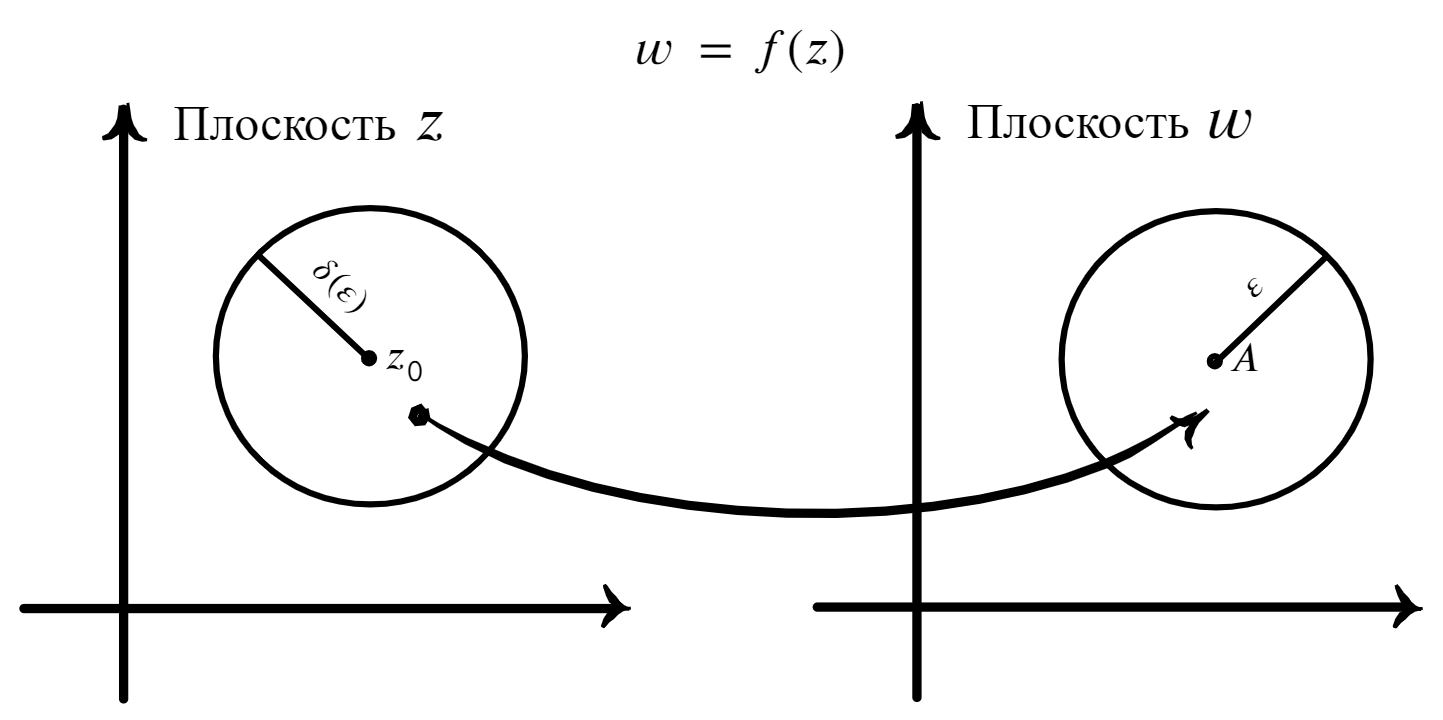
\includegraphics[scale=0.5]{images/016.png}$$
Когда мы говорим о пределе функции, мы рассматриваем лишь однозначные функции.\\\\
Число $A$ может быть и $\infty$. Пусть $A = \infty$, тогда $f\underset{z\to \infty}{\longrightarrow}\infty$, если $$\limdef\ \forall z : |z|\geqslant \delta (\epsilon) \Rightarrow |f(z)|\geqslant \epsilon.$$
\textbf{Теорема.}
	$f(z)\underset{z\to z_0}{\longrightarrow}A = B + i\cdot D \Longleftrightarrow u(x,y)\underset{\underset{y\to y_0}{x\to x_0}
	}{\longrightarrow}B$, $v(x,y)\underset{\underset{y\to y_0}{x\to x_0}}{\longrightarrow}D$.\\\\
Пусть $z_0$ --- предельная точка множества $D$, а $w = f(z)$.\\\\
$\bullet$ \textit{Число $A$ --- \textbf{предел функции} $f(z)$ при $z \to z_0$ \textbf{вдоль множества} $D$, если} $$\limdef,\ \forall z \in D\backslash\{z_0\} : 0 < |z-z_0|\leqslant\delta(\epsilon)\Rightarrow |f(z) - A|\leqslant\epsilon.$$
Тогда пишут $\lim\limits_{\underset{z\in D}{z\to z_0}}f(z) = A$.\\\\
\textit{\textbf{Свойства предела функции:}}\begin{enumerate}
	\item \textbf{\textit{Единственность.}} \textit{Предел функции, если он существует, определен однозначно.}
	\item \textit{Если $f(z)\underset{z\to z_0}{\longrightarrow} A\in \Cm$, то функция ограничена в некоторой проколотой окрестности точки $z_0$.}
	\item \textit{Если $\lim\limits_{z\to z_0}f(z) = A$, $\lim\limits_{z\to z_0}f(z) = B$, $A, B\in\Cm$, то}\begin{enumerate}
		\item $\lim\limits_{z\to z_0}\Big(f(z) + g(z)\Big) = \lim\limits_{z\to z_0}f(z) + \lim\limits_{z\to z_0}g(z);$
		\item $\lim\limits_{z\to z_0}\Big(f(z) \cdot g(z)\Big) = \lim\limits_{z\to z_0}f(z) \cdot  \lim\limits_{z\to z_0}g(z);$
		\item $\lim\limits_{z\to z_0}\dfrac{f(z)}{g(z)} = \dfrac{\lim\limits_{z\to z_0}f(z)}{\lim\limits_{z\to z_0}g(z)},$ \textit{если} $\lim\limits_{z\to z_0}g(z)\ne 0$.
	\end{enumerate}
\end{enumerate}
Пишем $f(z)\underset{z\to z_0}{\sim}g(z)$, если $\lim\limits_{z\to z_0}\dfrac{f(z)}{g(z)} = 1.$\\\\
Пишем $f(z)\underset{z\to z_0}{=}o(g(z))$, если $\lim\limits_{z\to z_0}\dfrac{f(z)}{g(z)} = 0.$\\\\
При вычислении пределов функцию можно также заменить на эквивалентную ей.\\\\
Рассмотрим функцию $w = f(z)$ определенную в окрестности точки $z_0\in D$ (внутренняя точка). \\\\
$\bullet$ \textit{Функцию $f(z)$ называют \textbf{непрерывной в точке} $z_0$, если} $$\lim\limits_{z\to z_0} f(z) = f(z_0).$$
$\bullet$ \textit{Если точка $z_0 \in D$ является предельной, то при $\lim\limits_{z\to z_0} f(z) = f(z_0)$ функция $f$ \textbf{непрерывна в точке $z_0$ вдоль множества $D$}.}\\\\
Любую функцию можно записать в виде $$w = f(z) = u(x,y) + i\cdot v(x,y).$$
Функция $f(z)$ непрерывна в точке $z_0$ $\Longleftrightarrow$ $u(x,y)$, $v(x,y)$ непрерывны в точке $(x_0,y_0)$, где $x_0 + i\cdot y_0 = z_0$ (следует из определения).\\\\
\textbf{\textit{Свойства непрерывных функций:}}\begin{enumerate}
	\item \begin{enumerate}
		\item $f(z) + g(z)$ \textit{непрерывна};
		\item $f(z)\cdot g(z)$ \textit{непрерывна};
		\item $\dfrac{f(z)}{g(z)}$ \textit{непрерывна} ($g(z)\ne 0$),
	\end{enumerate}
	\textit{если функции $f(z)$ и $g(z)$ непрерывны в точке $z$.}
	\item \textit{Если $w = F(z)$, $z = \varphi(\zeta)$, причем $\varphi(\zeta)$ непрерывна в точке $\zeta_0$, а $F(z)$ непрерывна в точке $z_0 = \varphi(\zeta_0)$, то $F(\varphi(\zeta))$ непрерывна в точке $\zeta_0$ (композиция непрерывных функций является функцией непрерывной).}
	\item \textbf{(Теорема Кантора.)}\\
	\textit{Непрерывная на компакте $D$ функция $w = f(z)$ равномерно непрерывна, то есть }$$\limdef,\ \forall z',z'' \in D : |z' - z''|\leq\delta(\epsilon)\Rightarrow |f(z') - f(z'')|\leq \epsilon.$$
\end{enumerate}
\section{Дифференцирование комплексных функций.}
Пусть $w = f(z)$ определена в окрестности точки $z_0$. Построим приращение $$\Delta f = f(z_0 + \Delta z) - f(z_0).$$
$\bullet$ \textit{\textbf{Производной комплексной функции} называется предел (если он конечен) }$$\lim\limits_{\Delta z\to 0}\dfrac{\Delta f}{\Delta z} = f'(z_0) = f'(z)|_{z=z_0}.$$
Тогда будем говорить, что комплексная функция имеет конечную производную.\\\\
$\bullet$ \textit{Функцию $w = f(z)$ называют \textbf{дифференцируемой} в точке $z_0$, если} $\exists A \in \Cm :$ $$\Delta f = A\cdot \Delta z + o(\Delta z).$$
\textbf{Первый критерий дифференцируемости функции.} \textit{Фукнция $f(z)$ дифференцируема в точке $z_0$ $\Longleftrightarrow$ она имеет конечную производную в этой точке $f'(z_0)$.}\\\\
\begin{Proof}
	$\Rightarrow)$ Поскольку $\Delta f = A\cdot \Delta z  + o(\Delta z)$, то
	$$\dfrac{\Delta f}{\Delta z} = A + \dfrac{o(\Delta z)}{\Delta z}.$$
	Переходим к пределу при $\Delta z \to 0$:
	$$\lim\limits_{\Delta z \to 0}\dfrac{\Delta f}{\Delta z} = A\Rightarrow f'(z_0) = A.$$
	$\Leftarrow)$ $\lim\limits_{\Delta z\to 0}\dfrac{\Delta f}{\Delta z} = f'(z_0)$. Отсюда $$\lim\limits_{\Delta z\to 0}\Big(\dfrac{\Delta f}{\Delta z} - f'(z_0)\Big) = 0;$$
	$$\dfrac{\Delta f}{\Delta z} - f'(z_0) = o(1);$$
	$$\Delta f = f'(z_0)\cdot \Delta z + \Delta z \cdot o(1) = f'(z_0)\cdot \Delta z +o(\Delta z ),$$ 
	то есть функция дифференцируема в точке $z_0$.
\end{Proof}\\\\
\textbf{Замечание.} \textit{$o(\Delta z) = o(|\Delta z|)$, докажем это.} $$o(\Delta z) = \alpha (\Delta z) \Rightarrow \lim\limits_{\Delta z \to 0} \dfrac{\alpha (\Delta z)}{\Delta z} = 0;\eqno (*)$$
$$o(|\Delta z|) = \alpha (|\Delta z|) \Rightarrow \lim\limits_{\Delta z \to 0} \dfrac{\alpha (|\Delta z|)}{|\Delta z|} = 0.\eqno (**)$$
\textit{Тогда} $$\lim\limits_{\Delta z \to 0}\dfrac{\alpha (\Delta z)}{\Delta z} = \lim\limits_{\Delta z\to 0}\dfrac{\alpha (\Delta z)}{\Delta z}\cdot \dfrac{\Delta z}{|\Delta z|} = 0.$$
\textit{Соответственно, если выполняется $(*)$, то выполняется и $(**)$, и наоборот. Из этого следует, что дифференциал можно также записать в виде} $$\Delta f = A\cdot \Delta z + o(|\Delta z|).$$
\textbf{Второй критерий дифференцируемости функции.} \textit{Функция $f(z) = u(x,y) + i\cdot v(x,y)$ дифференцируема в точке $z_0 = x_0 + i\cdot y_0$ $\Longleftrightarrow$ \begin{enumerate}
		\item функции $u(x,y)$, $v(x,y)$ дифференцируемы в точке $(x_0,y_0)$;
		\item выполняются условия Коши-Римана: в точке $(x_0, y_0)$
		$$\dfrac{\d u}{\d x} = \dfrac{\d v}{\d y},\quad \dfrac{\d u}{\d y} = -\dfrac{\d v}{\d x}.$$
\end{enumerate}
Причем $$f'(z)|_{z=z_0} = \dfrac{\d u}{\d x}\Big |_{(x_0,y_0)} + i\cdot \dfrac{\d v}{\d x}\Big |_{(x_0,y_0)}.$$}
\begin{Proof}
	$\Rightarrow)$ $\Delta f = A\cdot \Delta z + o(\Delta z)$, где $$A = B_1 +i\cdot B_2,$$ $$\Delta f = \Delta u + i\cdot \Delta v,$$ $$\Delta z = \Delta x + i\cdot \Delta y,$$ $$o(\Delta z) = \epsilon_1 + i\cdot \epsilon_2.$$ Тогда $$\Delta f = \Delta u + i\cdot \Delta v = (B_1 + i\cdot B_2)(\Delta x + i\cdot \Delta y) + \epsilon_1 + i\cdot \epsilon_2.$$
	Приравняем вещественные и мнимые части $$\Delta u = B_1\Delta x - B_2\Delta y + \epsilon_1,\quad \Delta v = B_2\Delta x + B_1\Delta y + \epsilon_2;$$
	причем $|\epsilon_1|\leqslant |o(\Delta z)|$, $|\epsilon_1| = o(|\Delta z|) = o(\sqrt{(\Delta x)^2 + (\Delta y)^2})$. Аналогично $|\epsilon_2| =  o(\sqrt{(\Delta x)^2 + (\Delta y)^2})$. Подставим и получим $$\Delta u = B_1\Delta x - B_2\Delta y + o(\sqrt{(\Delta x)^2 + (\Delta y)^2}),\quad \Delta v = B_2\Delta x + B_1\Delta y + o(\sqrt{(\Delta x)^2 + (\Delta y)^2}).$$
	Вспомним, что\\\\
	\textit{Функция $f(x,y)$ называется дифференцируемой в точке $(x_0,y_0)$, если $\exists A,D\in \Rm : $ $$\Delta f = A\cdot \Delta x + D\cdot \Delta y + o(\sqrt{(\Delta x)^2 + (\Delta y)^2}),$$
	причем $A = f'_x$, $D = f'_y$.}\\\\
	Тогда $u(x,y)$ является дифференцируемой в точке $(x_0,y_0)$ и $$\dfrac{\d u}{\d x} = B_1,\quad \dfrac{\d u}{\d y} = -B_2.$$
	Но $v(x,y)$ также является дифференцируемой в точке $(x_0,y_0)$ и$$\dfrac{\d v}{\d x} = B_2,\quad \dfrac{\d v}{\d y} = B_1.$$
	Следовательно, $$\dfrac{\d u}{\d x} = \dfrac{\d v}{\d y},\quad \dfrac{\d u}{\d y} = -\dfrac{\d v}{\d x}.$$
	$\Leftarrow)$ Для доказательства все рассуждения проведем в обратном порядке. Так как $u(x,y)$ и $v(x,y)$ дифференцируемы в точке $(x_0,y_0)$, то в этой точке $$\Delta u = \dfrac{\d u}{\d x}\Delta x + \dfrac{\d u}{\d y}\Delta y + o_1(\sqrt{(\Delta x)^2 + (\Delta y)^2}),$$
	$$\Delta v = \dfrac{\d v}{\d x}\Delta x + \dfrac{\d v}{\d y}\Delta y + o_2(\sqrt{(\Delta x)^2 + (\Delta y)^2}).$$
	Тогда\begin{multline*}
		\Delta f = \Big(\dfrac{\d u}{\d x}\Delta x+ i\cdot \dfrac{\d v}{\d x}\Delta x\Big) + \Big(-\dfrac{\d v}{\d x}\Delta y + i\cdot \dfrac{\d u}{\d x}\Delta y\Big) + \underbrace{o_1(\sqrt{(\Delta x)^2 + (\Delta y)^2}) + o_2(\sqrt{(\Delta x)^2 + (\Delta y)^2})}_{o(\Delta z)}=\\=\dfrac{\d u}{\d x}\underbrace{(\Delta x + i\cdot \Delta y)}_{\Delta z} + i\cdot \dfrac{\d v}{\d x}\underbrace{(\Delta x + i\cdot \Delta y)}_{\Delta z} + o(\Delta z) = \Big(\dfrac{\d u}{\d x} + i\cdot \dfrac{\d v}{\d x}\Big)\cdot \Delta z + o(\Delta z).
	\end{multline*}
Следовательно, $f(z)$ дифференцируема в точке $z_0$, а $$f'(z_0) = \dfrac{\d u}{\d x}\Big |_{(x_0,y_0)} + i\cdot \dfrac{\d v}{\d x}\Big |_{(x_0,y_0)}.$$
\end{Proof}\\
Все производные от комплексных функций определяются аналогично вещественным функциям.\\\\
$\bullet$\textit{ Функция называется \textbf{дифференцируемой в области} $D$, если она дифференцируема в каждой точке этой области.}\\\\
\textbf{\textit{Свойства производных комплексных функций:}}
\begin{enumerate}
	\item \textit{Пусть $f(z)$ и $g(z)$ --- функции дифференцируемые в точке $z_0$. Тогда }\begin{enumerate}
		\item $(f(z)\pm g(z))' = f'(z) \pm g'(z)$;
		\item $(f(g)\cdot g(z))' = f'(z)\cdot g(z) + f(z)\cdot g'(z)$;
		\item $\Big(\dfrac{f(z)}{g(z)}\Big)' = \dfrac{f'(z)\cdot g(z) - f(z)\cdot g'(z)}{g^2(z)}$, если $g(z_0) \ne 0$.
	\end{enumerate}
	\textit{Все эти функции дифференцируемыe в точке $z_0$.}
	\item \textit{Если функция $w = f(z)$ дифференцируема в точке $z_0$, а $z = h(\zeta)$ дифференцируема в точке $\zeta_0$, причем $h(\zeta_0) = z_0$, то }$$(f(h(\zeta)))'\Big|_{\zeta_0} = f'(z_0)\cdot h'(\zeta_0).$$
\end{enumerate}
Так как производная и первый критерий дифференцирования совпадают с соответствующими утверждениями для вещественных функций, то и доказательства данных свойств совпадают с доказательствами соответствующих свойств для вещественных функций.
\section{Сопряженно-гармонические функции.}
Рассмотрим соотношение для вещественной функции $u = u(x,y)$ $$\dfrac{\d ^2 u}{\d x ^2} + \dfrac{\d^2 u}{\d y^2} = 0.\eqno(1)$$
$\bullet$ \textit{Уравнение $(1)$ называется \textbf{уравнением Лапласа} для функции $u(x,y)$.}\\\\
$\bullet$ \textit{Любая функция определенная в некоторой области и удовлетворяющая уравнению Лапласа в этой области называется \textbf{гармонической} функцией.}\\\\
Рассмотрим функцию $w = f(z)$ дифференцируемую в области $D$. Тогда $f(z) = u(x,y) + i\cdot v(x,y)$ и выполняются условия Коши-Римана $$\dfrac{\d u}{\d x} = \dfrac{\d v}{\d y},\quad \dfrac{\d u}{\d y} = -\dfrac{\d v}{\d x}.$$
Позже будет показано, что дифференцируемая в области функция является дважды непрерывно дифференцируемой. Из этого вытекает, что функции $u(x,y)$ и $v(x,y)$ дважды непрерывно дифференцируемы в области $D$. Получим $$u''_{xy} = v''_{y^2},\quad u''_{yx} = -v''_{x^2}.$$
По теореме о смешанных производных $u''_{xy} = u''_{yx}$. Следовательно, $$v''_{y^2} = - v''_{x^2} \Rightarrow v''_{x^2} + v''_{y^2} = 0,$$
то есть функция $v(x,y)$ гармоническая. Аналогично получим, что функция $u(x,y)$ также является гармонической. То есть, если комплексная функция дифференцируема, то вещественная и мнимая части этой функции --- гармонические функции.\\\\
$\bullet$ \textit{Пара гармонических функций $u(x,y)$ и $v(x,y)$ в области $D$ называется \textbf{сопряженно-гармонической}, если $u(x,y)$ и $v(x,y)$ --- вещественная и мнимая части дифференцируемой в области $D$ функции $f(z) = u(x,y) + i\cdot v(x,y)$.}\\\\
Зная одну из двух сопряженно-гармонических функций, всегда можно найти вторую.\\\\ Используя теорему о независимости КРИ-2 от пути интегрирования, покажем, что выражение $$-\dfrac{\d u}{\d y}dx + \dfrac{\d u}{\d x} dy$$
удовлетворяет условию Эйлера. Примем $P(x,y) = -u'_y$, $Q(x,y) = u'_x$. Тогда $$P'_{y} = -u''_{y^2},\quad Q'x = u''_{x^2}.$$
А условие $$-u''_{y^2} = u''_{x^2}$$ выполняется, так как функция $u(x,y)$ удовлетворяет уравнению Лапласа. Следовательно, $\exists v (x,y) = -\dfrac{\d u}{\d y}dx + \dfrac{\d u}{\d x} dy$ такая, что $v'_x = -u'_y$, $v'_y = u'_x$.
\section{Кривые.}
Пусть задана непрерывная комплекснозначная функция $z = z(t)$, $t \in [a,b]$. Тогда можно выделить вещественную и мнимую части $$z(t) = x(t ) + i\cdot y(t).$$
$\bullet$ \textit{Множество точек комплексной плоскости с координатами $z(t)$ при $t\in [a,b]$ называется \textbf{кривой}, а уравнение $z = z(t)$ называется \textbf{комплекснозначным параметрическим уравнением кривой}.}\\\\
\noindent
\parbox[b][4.5cm][t]{50mm}{
	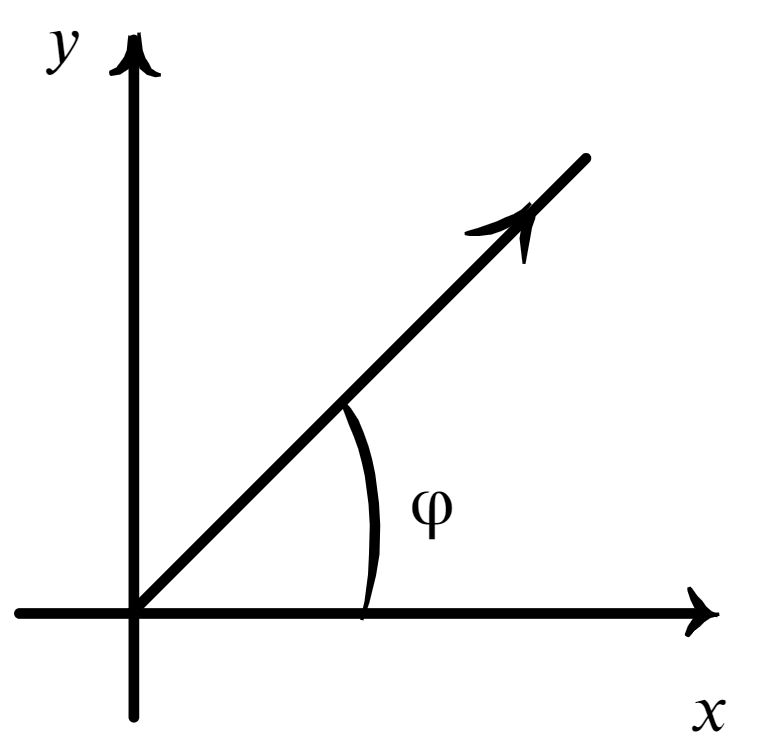
\includegraphics[scale=0.35]{images/017.png}}
\hfill
\parbox[b][4.5cm][t]{100mm}{
	Рассмотрим луч, выходящий из начала координат.\\\\
Покажем, что это кривая  и найдем ее комплекснозначное параметрическое уравнение. Пусть $\varphi \in (0;\dfrac{\pi}{2})$ и параметрическое уравнение $$\begin{cases}
	x = t,\\
	y = \tg \varphi \cdot t;
\end{cases}\quad t\in[0;+\infty)$$}\\
Тогда параметрическое комплекснозначное уравнение имеет вид $$z = t + i\cdot \tg \varphi \cdot t\quad \text{или}\quad z = t\cdot (\cos \varphi + i\cdot \sin \varphi),\quad  t\in [0;+\infty).$$

\noindent
\parbox[b][4.5cm][t]{50mm}{
	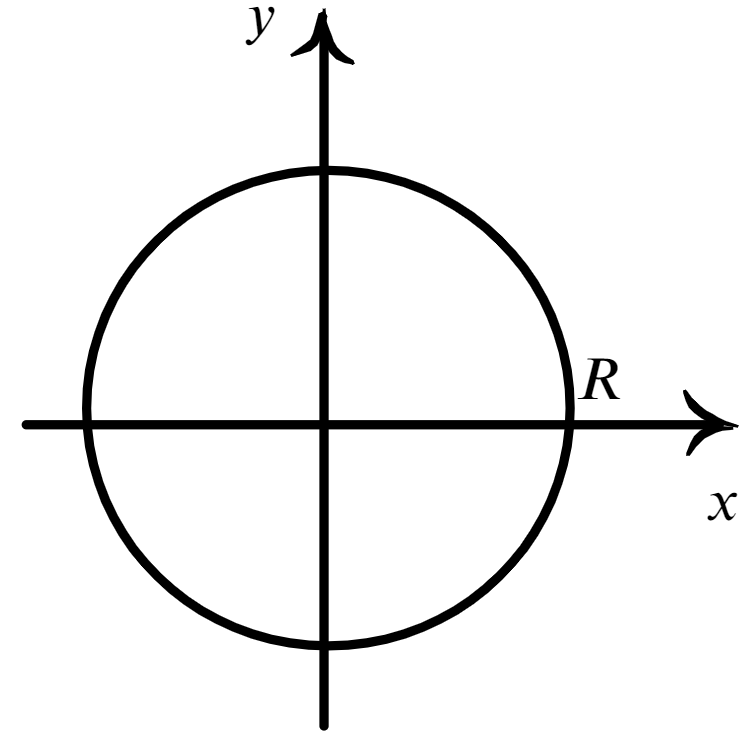
\includegraphics[scale=0.4]{images/018.png}}
	\hfill
	\parbox[b][4.5cm][t]{100mm}{
	Рассмотрим окружность радиуса $R$ с центром в начале координат. Ее параметрическое уравнение имеет вид $$\begin{cases}
	x = R\cdot \cos\varphi,\\
	y = R\cdot \sin\varphi;
\end{cases}\quad \varphi\in [0;2\pi].$$
Параметрическое комплекснозначное уравнение в таком случае имеет вид} $$z(\varphi) = R\cdot (\cos\varphi + i \cdot \sin\varphi) = R\ef{\varphi},\quad \varphi\in [0;2\pi].$$
$\bullet$ \textit{Кривая называется \textbf{гладкой}, если функция $z(t)$ непрерывно дифференцируема на $[a,b]$ и $|\dot{z}(t)|\ne 0$ $\forall t \in [a,b]$.}\\\\
Кривую без точек самопересечения будем называть \textbf{простой}. Длина простой гладкой кривой определяется формулой $$\text{дл.} l = \int\limits_a^b|\dot{z}(t)|dt.$$ 
\noindent
\parbox[b][5cm][t]{10mm}{
	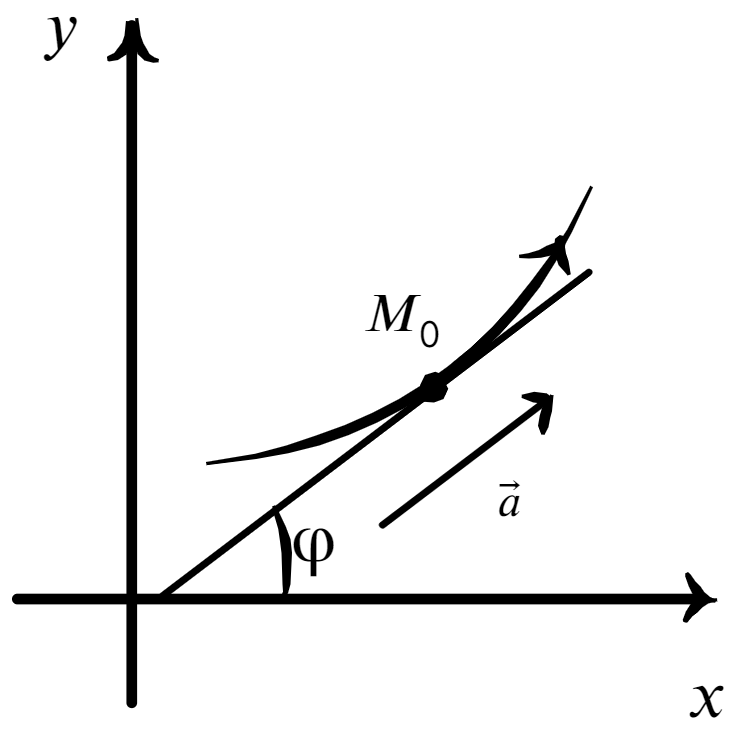
\includegraphics[scale=0.42]{images/019.png}}
\hfill
\parbox[b][4.5cm][t]{110mm}{Пусть задана гладкая кривая $$l: z= z(t) = x(t) + i\cdot y(t),\ t\in[a,b].$$ И пусть эта кривая ориентирована. К этой кривой проведена касательная через точку $M_0$ и параллельный ей вектор $a$, причем, так как $\dot{z}(t) = \dot{x}(t) + i\cdot \dot{y}(t)$, его координаты $a(\dot{x}(t), \dot y(t))$. Тогда угол $\varphi = \arg \dot z (t)$ --- это угол между касательной (вектором $a$) и осью $x$.}
\section{Интегрируемые функции комплексного переменного.}
Пусть $l$ --- гладкая кривая, имеющая комплекснозначное параметрическое уравнение $$l: z(t) = x(t) + i\cdot y(t),\ t\in[a,b].$$
И пусть на кривой $l$ задана функция однозначная $f(z)$.\\\\
$\bullet$ \textit{Тогда интеграл от комплекснозначной функции $$\intab f(z(t))\cdot \dot z (t) dt := \int\limits_l f(z)dz$$ называется \textbf{интегралом от комплексной функции} $f(z) = u(x,y) + i \cdot v(x,y)$.}\\\\
Следовательно, \begin{multline*}
	\intab f(z(t))\cdot \dot z (t) dt = \intab\Big(u(x(t),y(t)) + i\cdot v(x(t),y(t)))\Big)\cdot \Big(\dot x(t) + i\cdot \dot y(t)\Big)dt =\\= \intab (u\dot x - v\dot y)dt + i\cdot \intab (u\dot y + v\dot x)dt= \int\limits_l udx - vdy + i\cdot \int\limits_l vdx + udy.
\end{multline*}
Отсюда $$\int\limits_l f(z)dz = \int\limits_l udx - vdy + i\cdot \int\limits_l vdx + udy.$$
\textbf{\textit{Свойства интеграла комплексного переменного:}}\begin{enumerate}
	\item \textit{Линейность.}
	$$\int\limits_l (\alpha f(z) + \beta g(z))dz = \alpha \intl f(z)dz + \beta \intl g(z)dz.$$
	\item \textit{Адиитивность.}\\\\
	Есди кривая $l$ кусочно-гладкая состоящая из кривых $\buildrel\,\,\frown\over{l_{i-1}l_i}$, то по определению $$\intl f(z)dz := \sum\limits_i\int\limits_{\buildrel\,\,\frown\over{l_{i-1}l_i}}f(z)dz.$$
	Если кривая $l$ состоит из кривых $\buildrel\,\,\frown\over{l_{j-1}l_j}$, $j = \overline{1,m}$, то по определению $$\intl f(z)dz := \sum\limits_j\int\limits_{\buildrel\,\,\frown\over{l_{j-1}l_j}}f(z)dz.$$
	\item Рассмотрим кусочно-гладкий путь $l: z= z(t),\ t\in[a,b].$ Тогда будем обозначать его через $l^+$. В свою очередь, путь $l^-: z= z(a+b-t),\ t\in[a,b]$ будем называть противоположно ориентированным по отношению к исходному пути.\\\\
	\textit{При замене ориентации пути на противоположную интеграл комплексного переменного меняет знак.}
	$$\int\limits_{l^+}f(z)dz = -\int\limits_{l^-}f(z)dz.$$
	\item \textit{Оценки интеграла комплексного переменного.}\begin{enumerate}
		\item $\Big|\intl f(z)dz\Big|\leq \intl |f(z)|ds$ --- КРИ-1.
		\begin{Proof}
			\begin{multline*}
				\Big|\intl f(z)dz\Big| = \Big|\intab f(z(t))\cdot\dot z (t)dt\Big|\leq \Big|\intab |f(z(t))|\cdot |\dot z (t)|dt\Big| =\\= \intab |u(x(t),y(t)) + i \cdot v(x(t),y(t))|\cdot \sqrt{\dot x^2 + \dot y^2}dt=\\ =\text{ [сведение КРИ-1 к определенному интегралу] } = \intl|f(z)|ds.
			\end{multline*}
		\end{Proof}
	\item $\Big|\intl f(z)dz\Big|\leq M\cdot \text{дл.}l$, где $M=\underset{z\in l}{\sup}|f(z)|$.
	\begin{Proof}
		$\Big|\intl f(z)dz\Big|\leq M\cdot \intl ds = M\cdot \text{дл.}l$
	\end{Proof}
	\end{enumerate}
\end{enumerate}
\section{Геометрический смысл модуля и аргумента производкой комплексной функции.}
Рассмотрим функцию $w = f(z)$ такую, что $f'(z_0) = \lim\limits_{\Delta z \to 0}\dfrac{\Delta f}{\Delta z}$. И рассмотрим гладкую кривую $l : z = z(t)$, $t\in [a,b]$. Образом этой кривой будет кривая $L: w=f(z(t))$, $t\in [a,b]$.
$$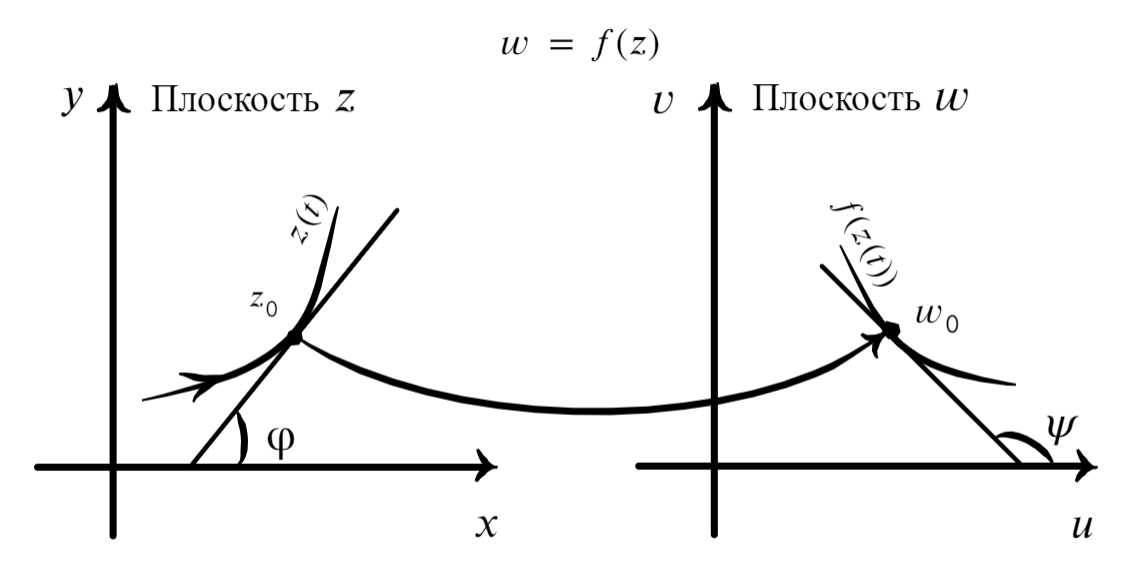
\includegraphics[scale=0.6]{images/020.png}$$
Обозначим $\varphi = \arg \dot z (t_0)$, где $t_0 \in [a,b]$, угол между касательной к кривой в точке $z_0 = z(t_0)$ и осью $x$. Найдем угол $\psi$ (угол между касательной к образу кривой в точке $w_0 = f(z(t_0))$). Так как
$$\Big(f(z(t))\Big)'\Big|_{t=t_0} = f'(z_0)\cdot z'(t_0),$$
то $$\psi = \arg(f'(z_0)\cdot z'(t_0)) = \arg z'(t_0)  + \arg f'(z_0) = \varphi + \arg f'(z_0).$$
То есть $\psi$ --- это угол, на который повернулась касательная к кривой при переходе к образу (при условии, что $f'(z_0) \ne 0$).\\\\
Если функция $f(z)$ дифференцируема в точке $z_0$ и $f'(z_0) \ne 0$, то при действии функции углы между кривыми сохраняются.\\\\
Рассмотрим окружность $$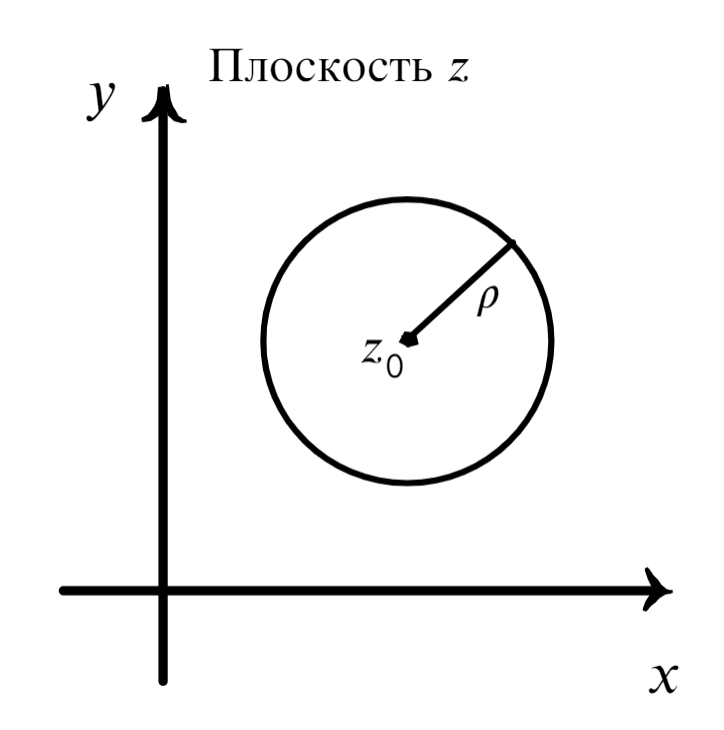
\includegraphics[scale = 0.5]{images/021.png}$$ Причем $|z-z_0| =|\Delta z|$ --- точки, лежащие на окружности. Тогда $$\dfrac{\Delta f}{\Delta z} = f'(z_0) + o(1),\quad f'(z_0) = \lim\limits_{\Delta z \to 0} \dfrac{\Delta f}{\Delta z}.$$
Тогда при действии функции $f(z)$ образом окружности будет замкнутая кривая, которая необязательно является окружностью.
$$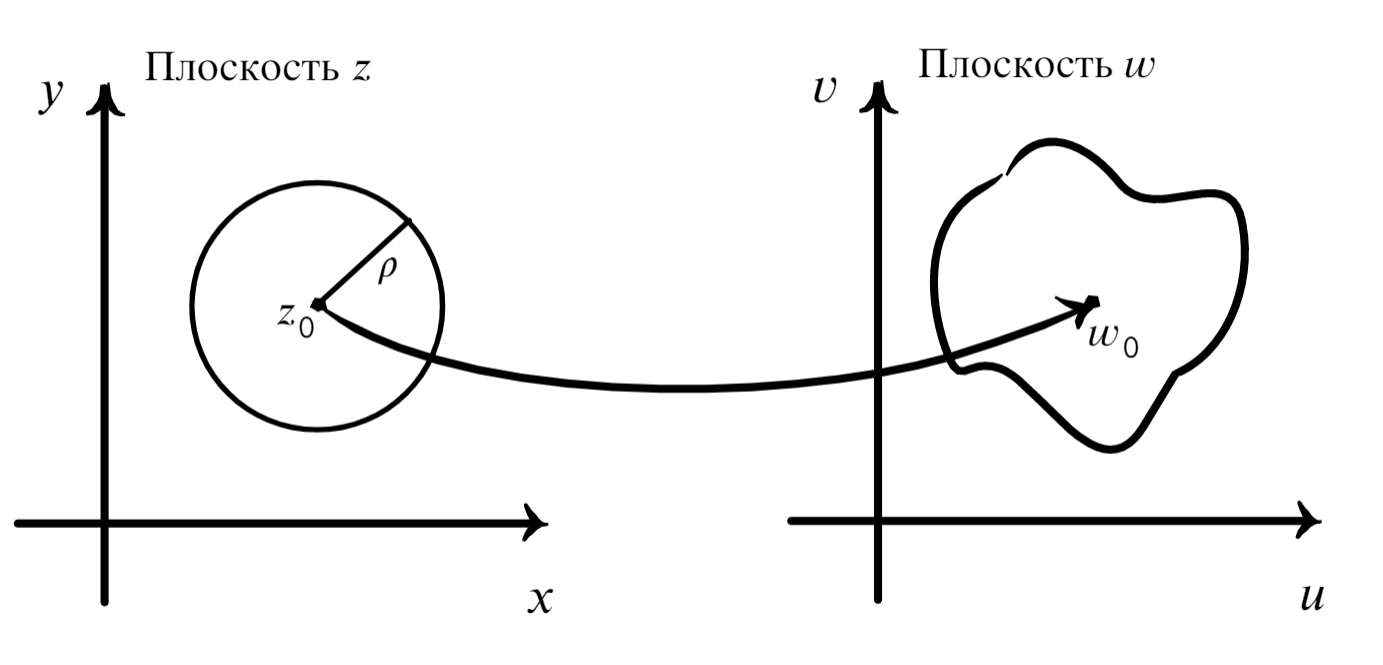
\includegraphics[scale = 0.6]{images/022.png}$$
При этом
$$|\Delta f|\approx |f'(z_0)|\cdot |\Delta z|.$$
Тогда с точностью до $o(1)$ получится окружность радиуса $\rho\cdot |f'(z_0)|$, однако при действии функции окружность изменится.\\\\
$\bullet$ \textit{Предел $\lim\limits_{\Delta z \to 0}\dfrac{|\Delta f|}{|\Delta z|}$ называется \textbf{коэффициентом растяжения} плоскости в точке $z_0$ при действии функции $w = f(z)$.}\\\\
Следовательно, $|f'(z_0)|$ --- коэффициент растяжения плоскости в точке $z_0$ при действии функции $w = f(z)$.\\\\
Пусть $D$ --- область в плоскости $z$, а $K$ --- образ этой области при действии функции $w = f(z) = u(x,y)+i\cdot v(x,y)$, $(x,y)\in D$.
$$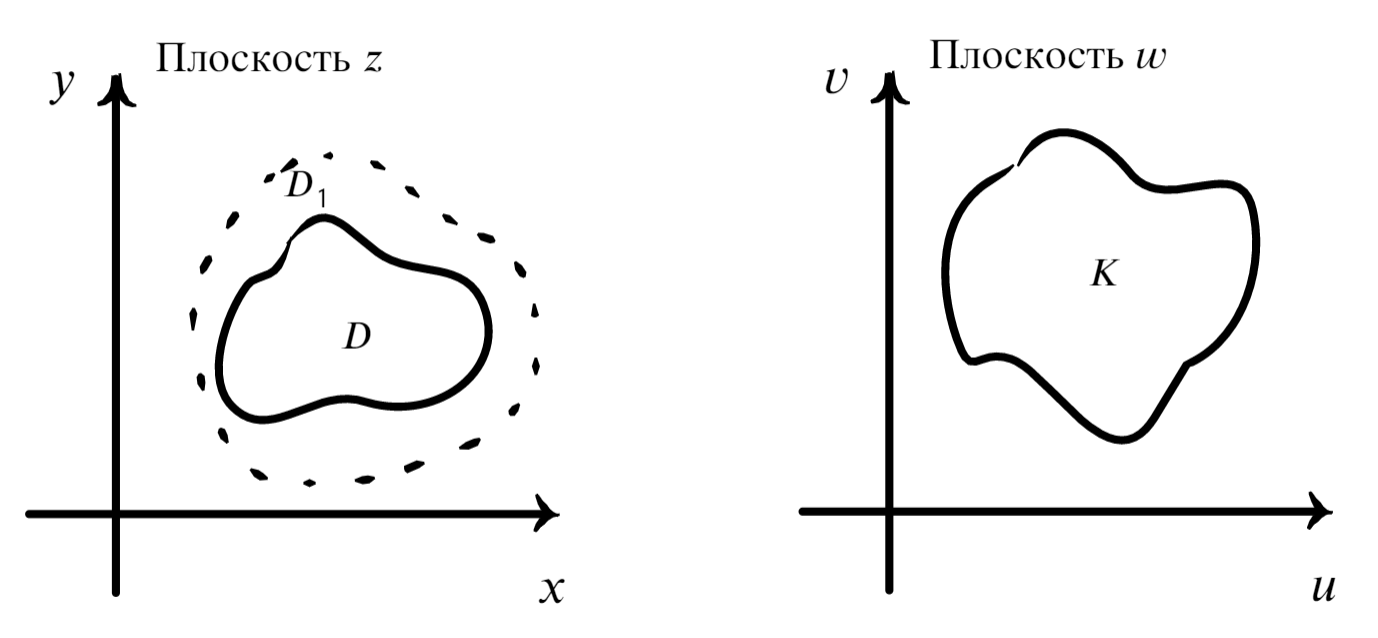
\includegraphics[scale = 0.6]{images/023.png}$$
Предположим, что отображение $\begin{cases}
	u = u(x,y),\\
	v = v(x,y)
\end{cases}$ --- диффеоморфное отображение области $D$ и области $K$. Тогда пл.$K = \iint\limits_D |\mathcal{I}|dxdy$, где $\mathcal{I}$ --- якобиан $$\mathcal{I} = \begin{vmatrix}
u'_x & u'_y\\
v'_x & v'_y
\end{vmatrix}.$$
Пусть $w = f(z)$ --- функция дифференцируема в некоторой области $D_1\supseteq D$ и $f'(z) \ne 0$ $\forall z \in D_1$. Так как функция дифференцируема, то выполняются условия Коши-Римана, то есть $u'_x = v'_y$, $u'_y = -v'_x$. Таким образом, $$\mathcal{I} = u'_xv'_y - u'_y v'_x = (u'_x)^2 + (v'_x)^2 = [f'(z) = u'_x + i\cdot v'_x] = |f'(z)|^2.$$
Тогда $$\text{пл.}K = \iint\limits_D |f'(z)|^2dxdy.$$
\section{Интегральная теорема Коши.}
\begin{theorem}
	Если функция $w = f(z)$ дифференцируема в односвязной области $D$, то $\forall$ замкнутой кусочно-гладкой кривой $l$ лежащей в области $D$ $$\intl f(z)dz = 0.$$ 
\end{theorem}\begin{Proof}
Если функция $f(z) = u(x,y) + i\cdot v(x,y)$ дифференцируема, то она непрерывно дифференцируема в области $D$ (доказательство этого утверждения приведем позже). То есть функции $u(x,y)$, $v(x,y)$ непрерывно дифференцируемы в области $D$. Тогда \begin{multline*}
	\intl f(z)dz = \intl (udx - vdy) + i\cdot \intl (vdx + udy) =\\= \text{[по теореме о независимости КРИ-2 от пути интегрирования]} =0.
\end{multline*}
Проверим выполнение условий примененной теоремы:
$$-\dfrac{\d v}{\d x} = \dfrac{\d u}{\d y},\quad \dfrac{\d v}{\d y} = \dfrac{\d u}{\d x},$$
а это условия Коши-Римана. По второму критерию дифференцируемости они выполняются, следовательно, выполняется теорема о независимости КРИ-2 от пути интегрирования.
\end{Proof}
\section{Следствия из интегральной теоремы Коши.}
\textbf{Следствия.}
\begin{enumerate}
	\item \textit{Если функция $w = f(z)$ дифференцируема в односвязной области $D$, то интеграл $\intl f(z)dz$ не зависит от формы кривой, лежащей в области $D$.}
	$$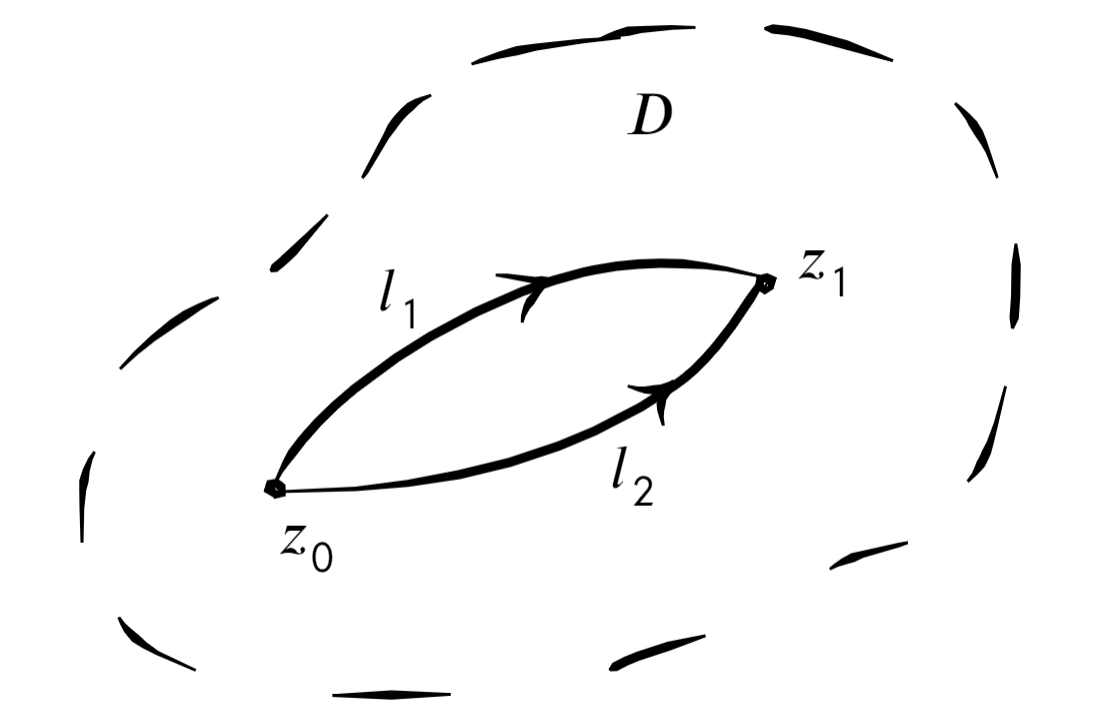
\includegraphics[scale=0.25]{images/024.png}$$
	Какую бы кривую мы не взяли, интегралы по $l_1$ и по $l_2$ будут совпадать.
	\item \textit{Если кривая $l_1$ получена из кривой $l_0$ путем непрерывной деформации, не выводящей из области $D$, и начало и конец этих кривых совпадают, а функция $w = f(z)$ дифференцируема в этой области, то $$\int\limits_{l_1} f(z)dz = \int\limits_{l_0}f(z)dz.$$
	Причем область необязательно односвязная.}
$$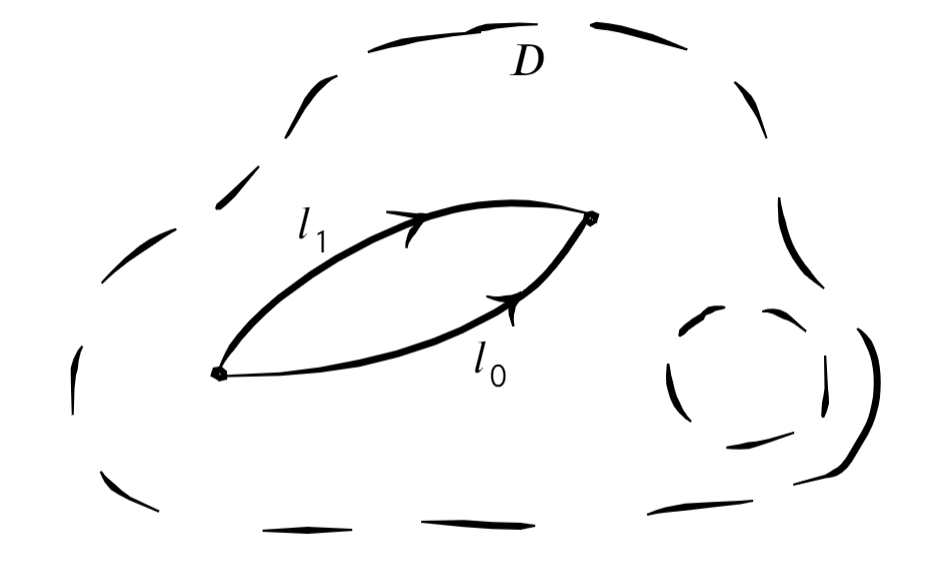
\includegraphics[scale=0.3]{images/025.png}$$
\begin{Proof}
	Всегда можно выбрать область $D_1$, которая односвязная и лежит в области $D$, такую, что $l_1$ и $l_0$ лежат в области $D_1$. Тогда получаем утверждение из следствия 1.
	$$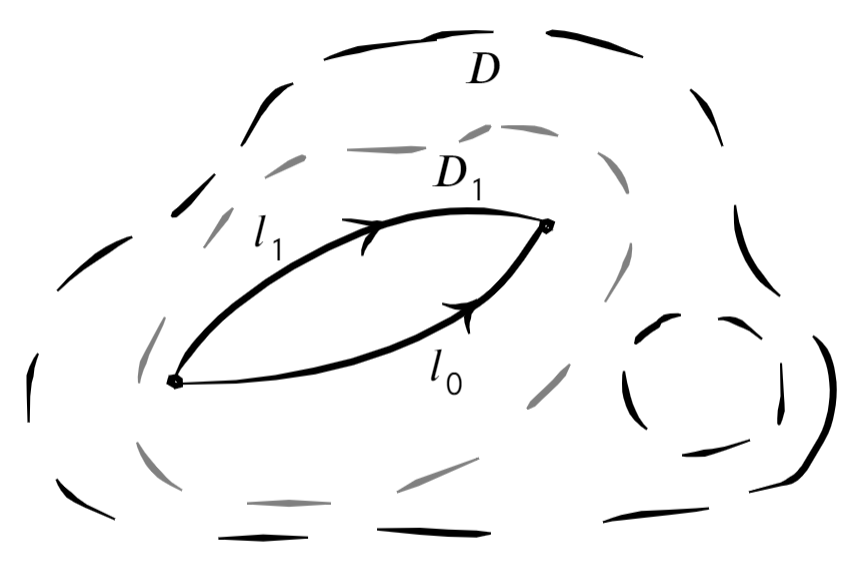
\includegraphics[scale=0.3]{images/026.png}$$
\end{Proof}\\
\noindent
\parbox[b][5cm][t]{10mm}{
	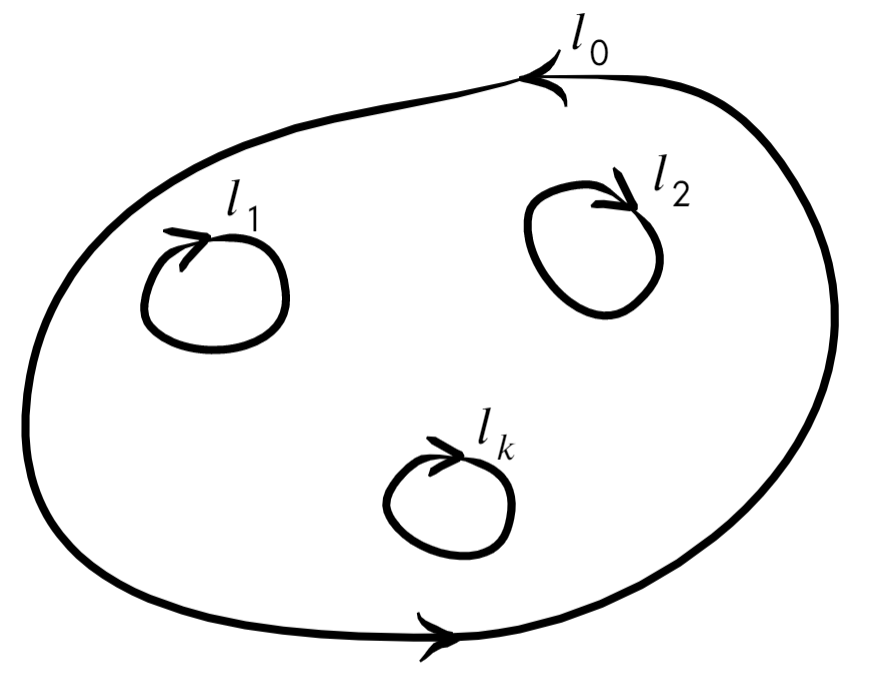
\includegraphics[scale=0.35]{images/027.png}}
\hfill
\parbox[b][4.5cm][t]{100mm}{$\bullet$ \textit{Неодносвязная область, ограниченная простой кусочно-гладкой кривой $l_0$ и простыми непересекающимися кусочно-гладкими кривыми $l_1$, $l_2$, $\ldots$, $l_k$, лежащими внутри кривой $l_0$ и ориентированными так, чтобы область оставалась справа, называется \textbf{стандартной многосвязной областью}.}}
\item \textit{Если функция $w = f(z)$ дифференцируемая в некоторой области $D$, содержит стандартную многосвязную область, то} $$\int\limits_{l_0} f(z)dz + \sum_{i = 1}^{k}\int\limits_{l_i}f(z)dz= 0.$$\begin{Proof}
	Проведем разрезы, соединяющие кривую $l_0$ с кривыми $l_1, l_2,\ldots, l_k$.\\\\
	\noindent
	\parbox[b][5cm][t]{10mm}{
		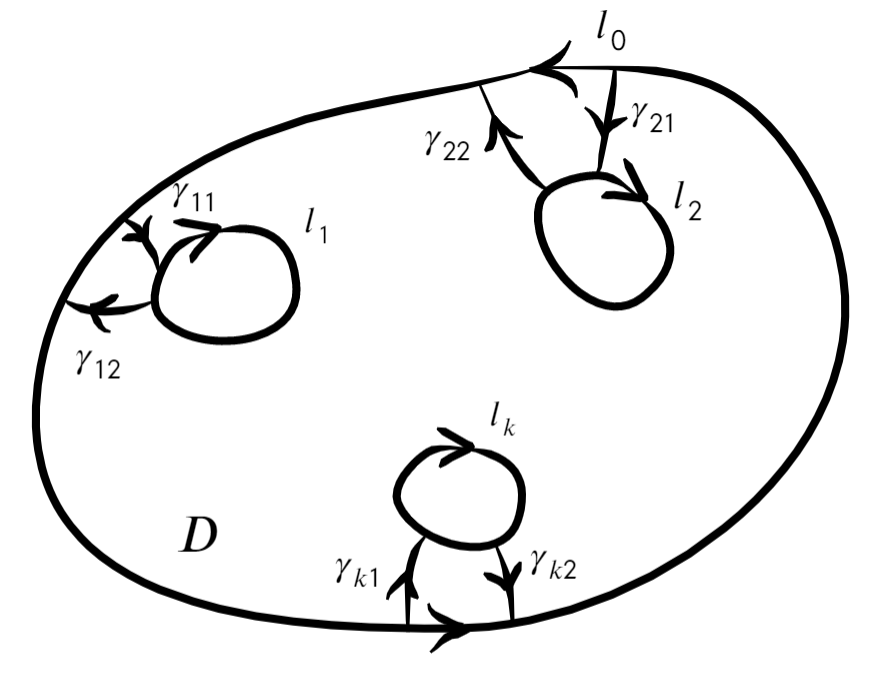
\includegraphics[scale=0.35]{images/028.png}}
	\hfill
	\parbox[b][4cm][t]{100mm}{Рассмотрим кривую $\Gamma$, образовавшуюся из кривых $l_0, l_1, \gamma_{11}, \gamma_{21}, \ldots, l_k, \gamma_{k1}, \gamma_{k1}$, и область ограниченную кривой $\Gamma$. Эта область односвязная. Функция $w = f(z)$ будем дифференцируема в этой области. Тогда по интегральной теореме Коши}\begin{multline*}
		\int\limits_{\Gamma} f(z)dz = 0 = \int\limits_{l_0} f(z)dz + \int\limits_{l_1} f(z)dz + \ldots + \int\limits_{l_k} f(z)dz + \underbrace{\int\limits_{\gamma_{11}} f(z)dz + \int\limits_{\gamma_{12}} f(z)dz}_{=0} +\\+ \ldots + \underbrace{\int\limits_{\gamma_{k1}} f(z)dz + \int\limits_{\gamma_{k2}} f(z)dz}_{=0} = \int\limits_{l_0} f(z)dz + \sum_{i = 1}^{k}\int\limits_{l_i}f(z)dz.
	\end{multline*}
\end{Proof}\\
\textbf{Замечание.} \textit{Если в следствии 3 все кривые считать ориентированными так, что указанная область $D$, ограниченная этими кривыми, остается слева, то} $$\int\limits_{l_0} f(z)dz =\sum_{i = 1}^{k}\int\limits_{l_i}f(z)dz.$$
$$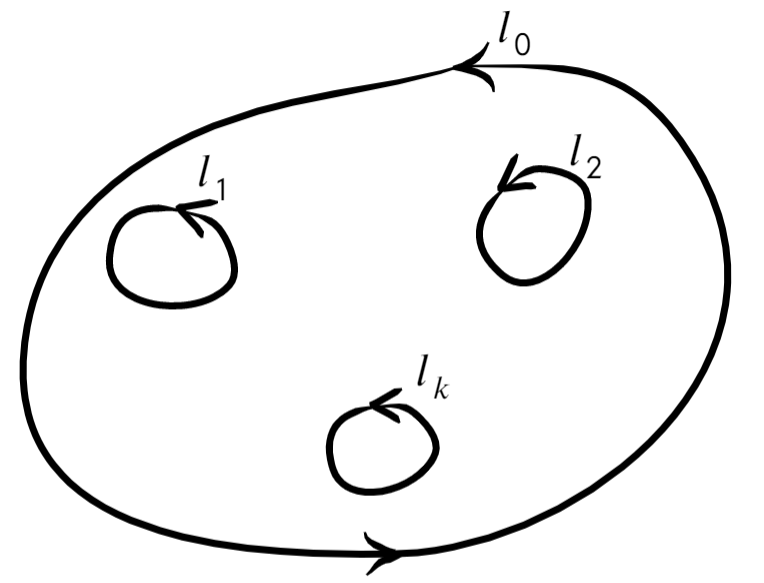
\includegraphics[scale=0.35]{images/029.png}$$
\item \textit{Если функция $w = f(z)$ дифференцируема в области $D$, а $l_0$ и $l_1$ --- две замкнутые кусочно-гладкие простые непересекающиеся кривые ориентированные так, что области ограниченные этими кривыми остаются слева, такие, что множество, лежащее между этими кривыми принадлежит области $D$, то} $$\int\limits_{l_0} f(z)dz = \int\limits_{l_1}f(z)dz.$$\begin{Proof}
	Вытекает из замечания к следствию 3.
	$$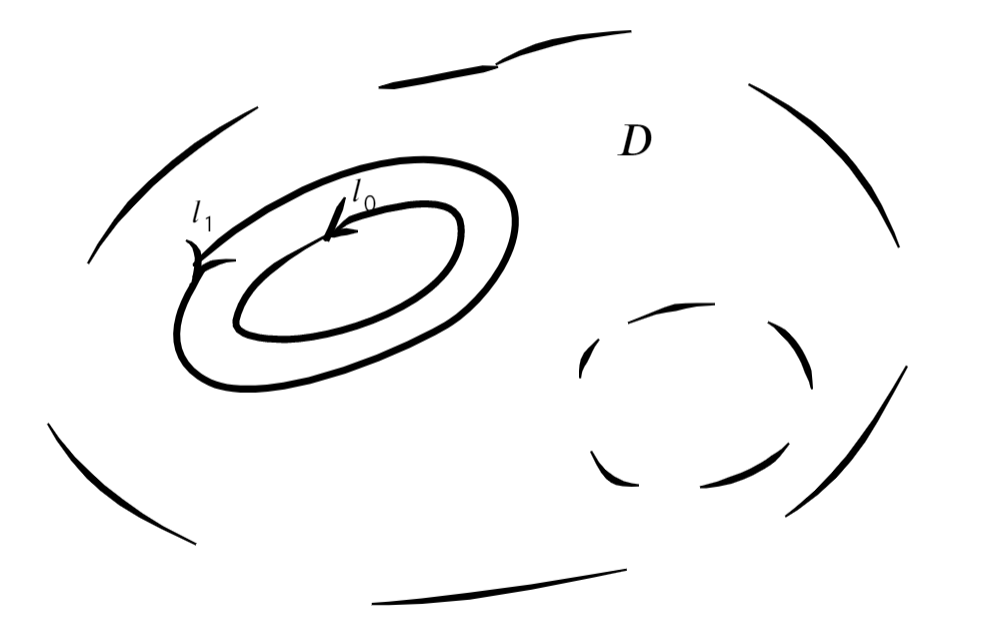
\includegraphics[scale=0.35]{images/030.png}$$
\end{Proof}\\
Также последнее следствие можно сформулировать следующим образом. Интеграл от дифференцируемой в области функции не меняется при деформации кривой, невыводящей кривую из области $D$.
\end{enumerate}
\section{Первообразная. Интеграл с переменным верхним пределом.}
Пусть функция $w = f(z)$ задана в области $D \subseteq \Cm$.\\\\
$\bullet$ \textit{Функция $F(z)$ заданная в области $D$ называется \textbf{первообразной} для функции $f(z)$, если $$F'(z) = f(z),\quad \forall z \in D.$$}
Если функция $f(z)$ задана в области $D$ и интеграл $\intl f(z)dz$ не зависит от формы кривой, лежащей в области $D$, то можно построить однозначную функцию $F(z) = \int\limits_{z_0}^z f(\zeta)d\zeta$, где $z_0$ --- некоторая фиксированная точка из $D$, а $z$ --- произвольная точка из $D$ ($\int\limits_{z_0}^z f(\zeta)d\zeta$ --- интеграл по кривой, соединяющей точки $z_0$ и $z$).\\\\
$\bullet$ \textit{Функция $$F(z) = \int\limits_{z_0}^z f(\zeta)d\zeta$$ называется \textbf{интегралом с переменным верхним пределом}.}\begin{theorem}
	[о первообразной] Если функция $f(z)$ дифференцируема в односвязной области $D$, то функция $F(z) = \int\limits_{z_0}^z f(\zeta)d\zeta$ является первообразной в области $D$ для функции $f(z)$.
\end{theorem}\begin{Proof}
Возможность построения однозначной функции $F(z)$ вытекает из  следствия 1 интегральной теоремы Коши. Необходимо доказать, что $\forall z \in D$ $F'(z) = f(z)$. Возьмем точки $z$, $z + \Delta z \in D$. Тогда \begin{multline*}
	F'(z) = \lim\limits_{\Delta z \to 0} \dfrac{\Delta F(z)}{\Delta z} = \lim\limits_{\Delta z \to 0} \dfrac{F(z + \Delta z) - F(z)}{\Delta z} = \lim\limits_{\Delta z \to 0} \dfrac{\int\limits_{z_0}^{z + \Delta z}f(\zeta)d\zeta - \int\limits_{z_0}^{z}f(\zeta)d\zeta}{\Delta z}=\\=\text{[из независимости от формы пути]} = \lim\limits_{\Delta z \to 0} \dfrac{\int\limits_{z}^{z + \Delta z}f(\zeta)d\zeta}{\Delta z}.
\end{multline*}
\begin{multline*}
	F'(z) - f(z) = \lim\limits_{\Delta z \to 0}\Big(\dfrac{1}{\Delta z}\int\limits_{z}^{z + \Delta z}f(\zeta)d\zeta - f(z) \Big) = \lim\limits_{\Delta z \to 0}\Big(\dfrac{1}{\Delta z}\int\limits_{z}^{z + \Delta z}f(\zeta)d\zeta - \dfrac{f(z)}{\Delta z} \int\limits_{z}^{z + \Delta z}d\zeta \Big) = \\ =\lim\limits_{\Delta z \to 0} \dfrac{1}{\Delta z} \int\limits_{z}^{z + \Delta z} \Big( f(\zeta) - f(z)\Big)d\zeta = \Big[ \dfrac{1}{|\Delta z|}\cdot \Big|\int\limits_{z}^{z + \Delta z} \Big( f(\zeta) - f(z)\Big)d\zeta\Big|\leq \big[\\ \text{функция дифференцируема, следовательно, непрерывна в точке } z, \text{то есть} \\ \limdef,\ \forall\zeta : |\zeta - z |\leq\delta (\epsilon) \Rightarrow |f(\zeta) - f(z)|\leq \epsilon \big] \leq \dfrac{1}{\Delta z}\epsilon\cdot |\Delta z| = \epsilon\Big] = 0.
\end{multline*}
\end{Proof}\\
\textbf{Замечание.} \textit{Если $F_1(z)$ и $F_2(z)$ --- две первообразные для функции $f(z)$ в односвязной области $D$, то $F_1(z) - F_2(z) = C\in \Cm$.}
\begin{theorem}
	[формула Ньютона-Лейбница]
	Если $f(z)$ дифференцируема в односвязной области $D$, то $$\int\limits_{z_0}^{z_1}f(\zeta)d\zeta = G(z) \Big| _{z_0}^{z_1},$$ где $G(z)$ --- некоторая первообразная для функции $f(z)$.
\end{theorem}\begin{Proof}
Пусть $$\int\limits_{z_0}^{z}f(\zeta)d\zeta = F(z).$$
Полагаем в этом равенстве $z = z_1$. Тогда $$\int\limits_{z_0}^{z_1}f(\zeta)d\zeta = F(z_1) = F(z_1) - F(z_0) =  G(z) \Big| _{z_0}^{z_1}.$$
\end{Proof}\\
\textbf{Формула интегрирования по частям.} \textit{Если $u(z)$, $v(z)$ --- две непрерывно дифференцируемые в односвязной области $D$ функции, то} $$\int\limits_{z_0}^{z_1}u(z)dv(z) = u(z)\cdot v(z)\Big| _{z_0}^{z_1} - \int\limits_{z_0}^{z_1}v(z)du(z).$$
\section{Интегральная формула Коши.}
\begin{theorem}
	Если функция $f(z)$ дифференцируема в односвязной области $D$ и $l$ --- замкнутая кусочно-гладкая простая кривая лежащая в $D$, $z_0$ --- точка лежащая внутри $l$, то $$\intl \dfrac{f(z)}{z - z_0}dz = 2\pi i f(z_0).$$
\end{theorem}\begin{Proof}
$$	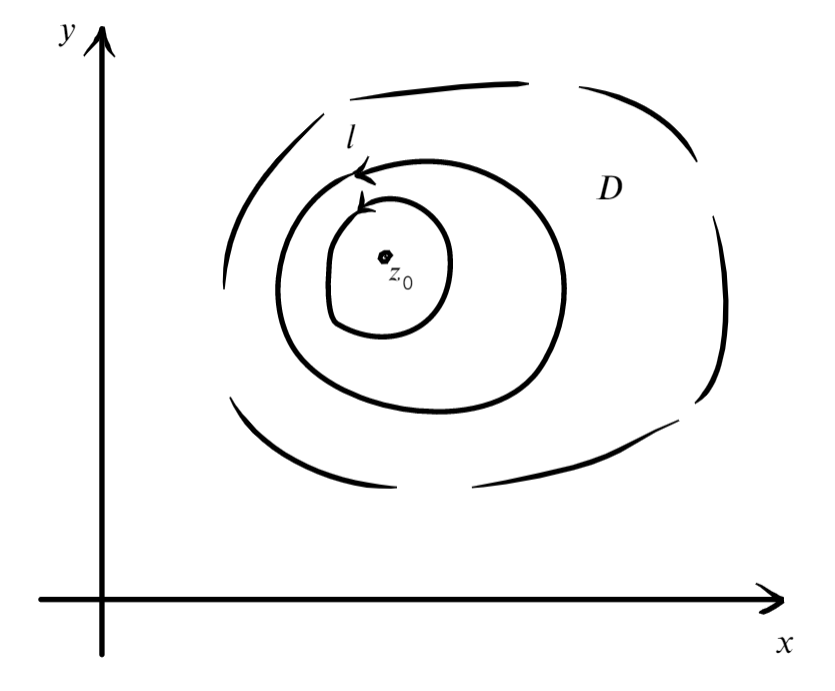
\includegraphics[scale=0.4]{images/032.png}$$
Возьмем окружность $C(z_0,\rho)$ с $\rho > 0$ таким, что окружность находится в области $D$. По следствию 2 из интегральной теоремы Коши $$\intl \dfrac{f(z)}{z-z_0}dz = \int\limits_{C(z_0,\rho)}\dfrac{f(z)}{z-z_0}dz.$$
$$\intl \dfrac{f(z)}{z-z_0}dz =\int\limits_{C(z_0,\rho)}\dfrac{f(z) - f(z_0) + f(z_0)}{z-z_0}dz  = \underbrace{\int\limits_{C(z_0,\rho)}\dfrac{f(z) - f(z_0)}{z-z_0}dz}_{I_1} + f(z_0)\int\limits_{C(z_0,\rho)}\dfrac{dz}{z-z_0}=$$
$$= I_1 +f(z_0)\cdot 2\pi i.$$
Покажем, что $I_1 = 0$. Функция $f(z)$ непрерывна в точке $z_0$, то есть $$\limdef, \forall z : |z-z_0|\leq \delta(\epsilon) \Rightarrow |f(z) - f(z_0)|\leq \epsilon.$$
Считаем, что $\rho \leq \delta(\epsilon)$. Оценим $|I_1|$:
$$|I_1| \leq \int\limits_{C(z_0,\rho)}\Big|\dfrac{f(z) - f(z_0)}{z-z_0}ds \Big|\leq \epsilon \int\limits_{C(z_0,\rho)}\dfrac{ds}{\rho} = 2\pi \epsilon.$$
Интеграл $I_1$ не зависит от радиуса $\rho$. Следовательно, $|I_1|\leq 	2\pi \epsilon$, $\forall\epsilon > 0$. Отсюда $I_1 = 0$. Тогда $$\intl \dfrac{f(z)}{z-z_0}dz =f(z_0)\cdot 2\pi i.$$
\end{Proof}
\begin{cor}
	Если функция $f(z)$ дифференцируема в области $D$ (необязательно односвязной) и $l, l_1$ --- две простые замкнутые кусочно-гладкие кривые, лежащие в $D$, $l_1$ лежит внутри $l$, $f(z)$ дифференцируема в области, ограниченной кривыми $l$ и $l_1$, $z_0$ лежит между кривыми $l$ и $l_1$, то $$\intl \dfrac{f(z)}{z-z_0}dz - \int\limits_{l_1}\dfrac{f(z)}{z-z_0}dz =f(z_0)\cdot 2\pi i.$$
\end{cor}\begin{Proof}
Соединим кривые $l$ и $l_1$ кривыми $\gamma_1^+$, $\gamma_1^-$.
Построим кривую $\Gamma$, состоящую из кривых $l$, $l_1$, $\gamma_1^+$, $\gamma_1^-$. Тогда $$ \int\limits_{\Gamma}\dfrac{f(z)}{z-z_0}dz = f(z_0)\cdot 2\pi i = \intl \dfrac{f(z)}{z-z_0}dz - \int\limits_{l_1}\dfrac{f(z)}{z-z_0}dz.$$
\end{Proof}
\begin{cor}
	Если функция $f(z)$ дифференцируема в односвязной области $D$, $l$ --- простая замкнутая кусочно-гладкая кривая, $z_0$ --- точка, не лежащая на кривой $l$, то $$\intl \dfrac{f(z)}{z-z_0}dz =\begin{cases}
		0,\ \text{если } z_0 \text{ не лежит внутри } l,\\
		2\pi i f(z_0),\ \text{если } z_0 \subset l. 
	\end{cases}$$
\end{cor}\begin{Proof}
Верхнее равенство вытекает из интегральной теоремы Коши. Нижнее равенство вытекает из интегральной формулы Коши.
\end{Proof}
\section{Степенные ряды.}
$\bullet$\textit{ Ряд $\sum\limits_{n = 0}^\infty c_n$, $c_n \in \Cm$ называется \textbf{комплексным числовым рядом.} }\\\\
$\bullet$ \textit{Число $P_n = \sum\limits_{k=0}^n c_k$ называется \textbf{частичной суммой комплексного числового ряда}.}\\\\
$\bullet$ \textit{Если $\exists \lim\limits_{n\to\infty} P_n = P \in \Cm$, то комплексный числовой ряд называется \textbf{сходящимся}, а число $P$ называтеся \textbf{суммой ряда}.}\\\\
Всегда можно записать $c_n = a_n + ib_n$, где $a_n$, $b_n \in \Rm$. Тогда ряд $\sumz c_n$ сходится $\Longleftrightarrow$ ряды $\sumz a_n$ и $\sumz b_n$ сходятся.\\\\
\textit{$\bullet$ Ряд $\sumz c_n$ \textbf{сходится абсолютно}, если сходится ряд $\sumz |c_n|$.}\\\\
\textit{$\bullet$ Ряд $\sumz c_n$ \textbf{сходится условно}, если расходится ряд $\sumz |c_n|$, но ряд $\sumz c_n$ сходится.}\\\\
$\bullet$ \textit{Ряд $\sumz c_n(z)$, где $c_n(z)$ --- комплексная функция определенная на множестве $D$, называется \textbf{функциональным комплексным рядом}. Множество точек $z\in \Cm$ таких, что ряд $\sumz c_n(z)$ сходится называется \textbf{множеством схоидмости} ряда.}\\\\
Пусть $D_1$ --- множество сходимости ряда $\sumz c_n$. Тогда $$\forall z \in D_1,\ \forall\epsilon > 0,\ \exists \delta(\epsilon, z) : \forall n \geq \delta(\epsilon, z) \Rightarrow \Big|\sum\limits_{k = n+1}^\infty c_k(z)\Big| \leq \epsilon$$ --- условие поточечной сходимости. Если выполняется условие $$ \forall\epsilon > 0,\ \exists \delta(\epsilon): \forall n \geq \delta(\epsilon),\ \forall z \in D_1  \Rightarrow \Big|\sum\limits_{k = n+1}^\infty c_k(z)\Big| \leq \epsilon,$$ то ряд $\sumz c_n(z)$ является равномерно сходящимся на $D_1$.
\begin{theorem}
	[о почленном интегрировании функционального ряда]
	Если члены ряда $\sumz c_n(z)$ непрерывны в области $D_0$ и ряд $\sumz c_n(z)$ сходится равномерно на некотором множестве $\overline{D} \subset D_0$, а кривая $l \in \overline{D}$, то возможно почленное интегрирование функционального ряда $$\intl \sumz c_n(z)dz = \sumz \intl c_n(z)dz.$$
\end{theorem}\begin{Proof}
Доказательство вытекает из соответствующей теоремы для вещественных функциональных рядов и определения интеграла от комплексной функции.
\end{Proof}\\\\
$\bullet$ \textit{Ряд $\sumz c_n\cdot (t-t_0)^n$, где $c_n \in \Cm$, называется \textbf{комплексным степенным рядом}.}\\\\
С помощью замены $t-t_0 = z$ комплексный степенной ряд можно привести к виду $\sumz c_nz^n.$ \\\\
Множество сходимостей комплексного степенного ряда не пусто, так как содержит по крайней мере одну точку $z = 0$.
\begin{lem}
	[Абеля]
	Если комплексный степенной ряд $\sumz c_nz^n$ сходится в точке $z_0 \ne 0$, то он сходится абсолютно в круге $|z| < |z_0|$ и сходится равномерно в любом круге $|z|\leq \rho$, где $\rho < |z_0|$.
\end{lem}\begin{Proof}
Ряд $\sumz c_nz_0^n$ сходится, то есть $c_nz_0^n \underset{n\to \infty}{\longrightarrow} 0$. Следовательно, $|c_nz_0^n| \underset{n\to \infty}{\longrightarrow} 0$. Тогда $\exists M> 0 : |c_nz_0^n| \leq M$.\\\\
Рассмотрим ряд из модулей $\sumz |c_nz^n| = \sumz |c_nz_0^n|\cdot \Big|\dfrac{z}{z_0}\Big|^n$.\\\\
Докажем, абсолютную сходимость. $$|c_nz_0^n|\cdot \Big|\dfrac{z}{z_0}\Big|^ \leq M\dfrac{|z|^n}{|z_0|^n}.$$
Если $|z|\leq |z_0|$, то $\Big|\dfrac{z}{z_0}\Big|<1$. Тогда ряд $\sumz M\Big|\dfrac{z}{z_0}\Big|^n$ сходится. Следовательно, ряд $\sumz c_nz^n$ сходится абсолютно в круге $B(0, |z_0|)$.\\\\
Докажем равномерную сходимость. $$|c_nz^n| \leq M\cdot \dfrac{\rho ^n}{|z_0|^n} = Mq^n.$$
Так как $q = \dfrac{\rho}{|z_0|}$, то ряд $\sumz Mq^n$ сходится, следовательно, ряд $\sumz c_nz^n$ равномерно сходится в круге $B(0,\rho)$ по признаку Вейерштрасса.
\end{Proof}\\\\
Пусть $L$ --- множество сходимостей комплексного степенного ряда.\\\\
$\bullet$ \textit{Число $\underset{z \in L}{\sup |z|} = R$ называется \textbf{радиусом сходимости} комплексного степенного ряда.}\\\\
Из леммы Абеля следует, что комплексный степенной ряд сходится в круге $|z|<R$ и расходится на множестве $|z| > R$. На окружности $|z| = R$ комплексный степенной ряд может быть как сходящимся, так и расходящимся.\\\\
Для нахождения радиуса сходимости можно использовать формулу Коши-Адамара $$R = \dfrac{1}{\overline{\lim\limits_{n \to \infty}} \sqrt[n]{|c_n|}}.$$
\section{Почленное дифференцирование комплексного степенного ряда.}
\begin{theorem}
	[о почленном дифференцировании степенного ряда]
	Если комплексный степенной ряд $\sumz c_nz^n$ имеет радиус сходимости $R>0$, то функция $f(z) =  \sumz c_nz^n$ является бесконечно дифференцируемой в круге $|z| < R$ и $m$-ая производная имеет вид $$f^{(m)}(z) = \sum\limits^\infty_{n = m} c_n \cdot n\cdot (n-1) \dots (n-m+1)\cdot z^{n-m},\ |z| < R, \forall m \in \N.$$
\end{theorem}\begin{Proof}
Рассмотрим ряд $S(z) = \sum\limits_{n=1}^\infty c_n\cdot n \cdot z^{n-1}$. Из формулы Коши-Адамара следует, что радиус сходимости этого ряда равен $$R_1 =  \dfrac{1}{\overline{\lim\limits_{n \to \infty}} \sqrt[n]{n\cdot |c_n|}} = R.$$
Следовательно, ряд, сходящийся в функции, $S(z)$ имеет тот же радиус сходимости, что и ряд, сходящийся к $f(z)$.\\\\
\noindent
\parbox[b][5cm][t]{10mm}{
	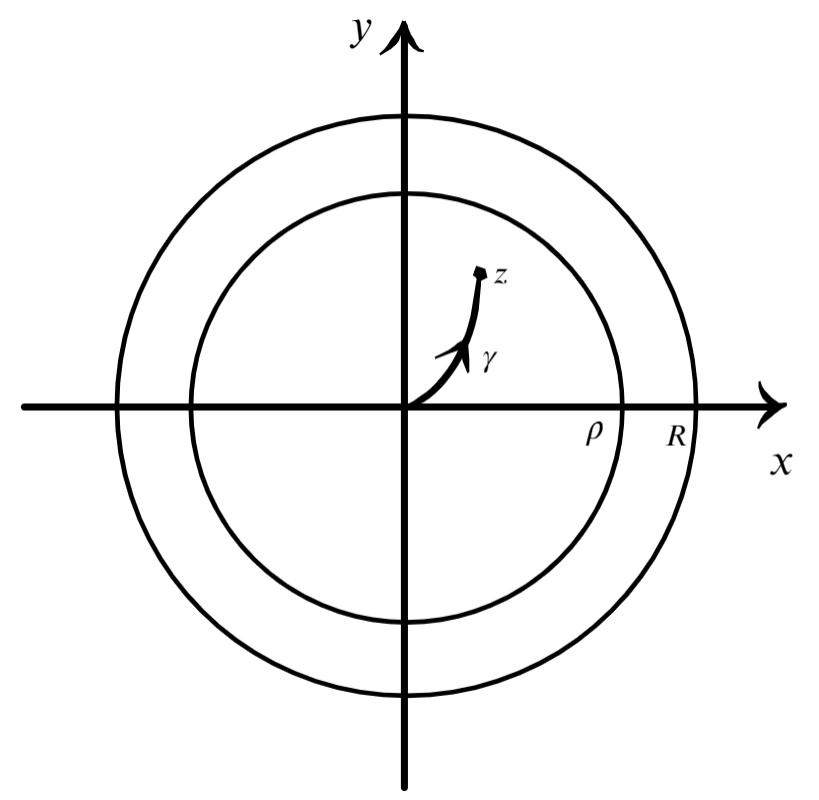
\includegraphics[scale=0.4]{images/034.png}}
\hfill
\parbox[b][4.5cm][t]{110mm}{
Возьмем окружность радиуса $\rho < R$. Тогда в круге $\overline{B}(0,\rho)$ ряд $\sum\limits_{n=1}^\infty c_n\cdot n \cdot z^{n-1}$ сходится равномерно по лемме Абеля. Возьмем произвольную точку $z$ и кривую $\gamma$, которая лежит в круге радиуса $\rho$ и соединяет точку $z$ с началом координат. Тогда интеграл $\int\limits_\gamma z^{n-1}dz$ не зависит от кривой интегрирования, так как функция $z^{n-1}$ дифференцируема на всей плоскости.}\\  Следовательно, $$\int\limits_\gamma z^{n-1}dz = \int\limits_0^z \zeta ^{n-1}d\zeta = \dfrac{z^n}{n}.$$ Ряд $\sumz c_n\cdot n \cdot z^{n-1}$ сходится равномерно на кривой $\gamma$. Тогда по теореме о почленном интегрировании $$\int\limits_\gamma \sumz c_n\cdot n\cdot z^{n-1}dz = \sumo c_n\cdot n\cdot \dfrac{z^n}{n} = \sumo c_nz^n = f(z) - c_0.$$
Причем интеграл слева не зависит от кривой интегрирования, следовательно $$\int\limits_0^z S(\zeta)d\zeta = f(z) - c_0.\eqno(1)$$
Используя доказательство теоремы о первообразной, можно доказать, что $\int\limits_0^z S(\zeta)d\zeta$ --- первообразная для функции $f'(z)$.\\\\
Из равенства (1) получаем, что функция $f(z)$ является первообразной для функции $S(z)$. Значит $f'(z) = S(z)$. Отсюда функция $f(z)$ является дифференцируемой в круге $B(0,\rho)$. А так как $\rho$ можно вызять сколь угодно близким к $R$, то функция $f(z)$ дифференцируема в круге $B(0,R)$. Тогда $$f'(z) = \sumo c_n\cdot n\cdot z^{n-1}.$$
Повторяя аналогичные рассуждения к функции $f'(z)$, можно показать, что через $(m-1)$ шагов получим $$f^{(m)}(z) = \sum\limits^\infty_{n = m} c_n \cdot n\cdot (n-1) \dots (n-m+1)\cdot z^{n-m}.$$
\end{Proof}\begin{cor}
Если сходится ряд $\sumo c_n(z-z_0)^n = f(z)$ и его радиус сходимости $R>0$, то $$c_n =  \dfrac{f^{(n)}(z_0)}{n!}.$$
\end{cor}\begin{Proof}
Полагаем $z = z_0$. Следовательно $c_0 = f(z_0)$. Продифференцируем функцию $f'(z)$ и получим $$f'(z) = \sumo c_n\cdot n\cdot (z-z_0)^{n-1}.$$
Пусть $z = z_0$, тогда $f'(z_0) = c_1\cdot 1$. Аналогичные действия проделаем $(m-1)$ раз. Тогда $$f^{(m)}(z_0) = c_m\cdot 1\cdot 2 \cdot \dots\cdot  m = c_m \cdot m!.$$
Отсюда $$c_m = \dfrac{f^{(m)}(z_0)}{m!}.$$
\end{Proof}\\
$\bullet$ \textit{Ряд $\sumz \dfrac{f^{(n)}(z_0)}{n!}(z-z_0)^n$ называется \textbf{рядом Тейлора} для комплексной функции $f(z)$.}\\\\
Из следствия вытекает, что если комплексная функция представима комплексным степенным рядом, то она разложима в ряд Тейлора.
\begin{cor}
	[единственность разложения функции в степенной ряд]
	Если функция $$f(z) = \sumz c_n(z-z_0)^n = \sumz b_n(z-z_0)^n$$ в круге $|z-z_0|<R$, $R \ne 0$, то $c_n = b_n$.
\end{cor}
\section{Регулярные функции.}
$\bullet$ \textit{Функция $f(z)$ называется \textbf{регулярной в точке} $z_0$, если} $$f(z) = \sumz c_n(z-z_0)^n,\quad \forall z : |z-z_0| < R,\ R>0.$$
То есть, иным словами, функция регулярна в точке $z_0$, если она разложима в степенной ряд по степеням $(z-z_0)$, сходящийся к функции $f(z)$ в некоторой окрестности точки $z_0$.\\\\
$\bullet$\textit{ Функция называется \textbf{регулярной в области}, если она регулярна в каждой точке этой области.}
\begin{theorem}
	[критерий регулярности функции в области]
	Функция $f(z)$ регулярна в области $D$ $\Longleftrightarrow$ функция $f(z)$ дифференцируема в области $D$.
\end{theorem}\begin{Proof}
$\Rightarrow)$ Если функция регулярна в области, то она разложима в степенной ряд в этой области. А сумма комплексного степенного ряда --- функция дифференцируема по теореме о почленном дифференцировании степенного ряда.\\\\
$\Leftarrow)$ Возьмем в области $D$ окружность $C(z_0,\rho)$ таким образом, чтобы она целиком лежала в области $D$. И возьмем произвольную точку $z$. $$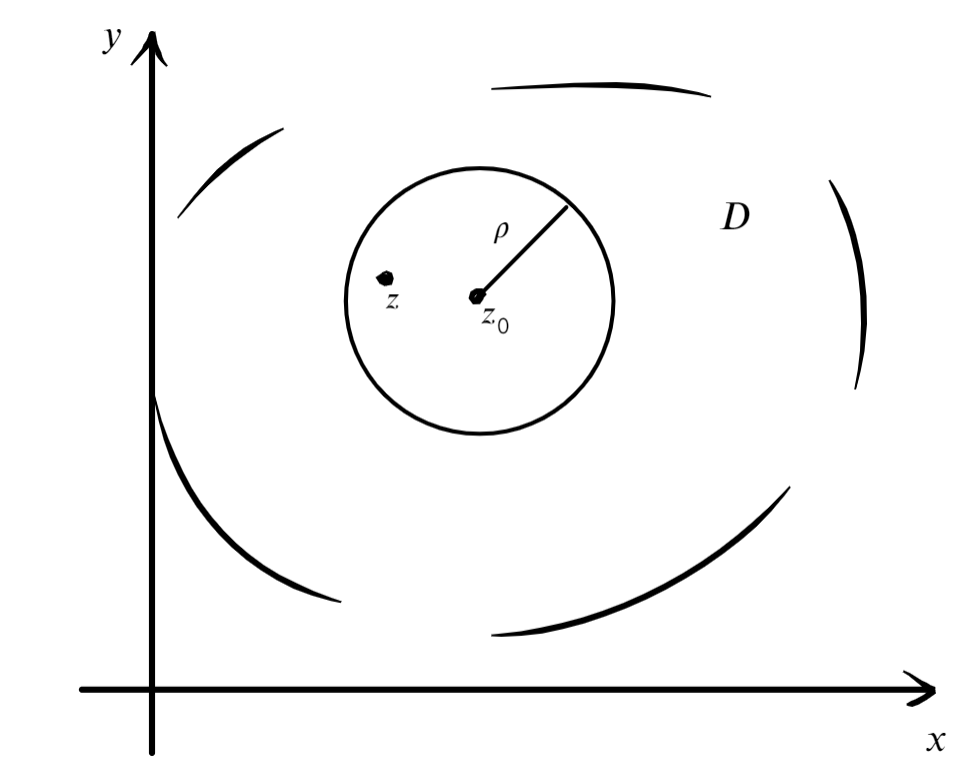
\includegraphics[scale = 0.45]{images/035.png}$$ Функция $f(z)$ дифференцируема в области $D$, значит дифференцируема и в окружности $C(z_0,\rho)$. По интегральной формуле Коши. $$f(z) = \dfrac{1}{2\pi i}\int\limits_{C(z_0,\rho)} \dfrac{f(\zeta)}{\zeta - z}d\zeta.$$
Разложим в степенной ряд функцию $\dfrac{1}{\zeta - z}$ по степеням $z - z_0$:
$$\dfrac{1}{\zeta - z} = \dfrac{1}{\zeta - z_0 + z_0 - z} = \dfrac{1}{(\zeta - z_0)(1 - \frac{z-z_0}{\zeta - z_0})} = \dfrac{1}{\zeta - z_0}\sumz\dfrac{(z-z_0)^n}{(\zeta - z_0)^n},$$
Причем $\dfrac{|z-z_0|}{|\zeta - z_0|} < 1$. И пусть $\zeta \in C(z_0,\rho)$. Следовательно, ряд $\sumz\dfrac{(z-z_0)^n}{(\zeta - z_0)^n}$ сходится равномерно на окружности $C(z_0,\rho)$ по признаку Вейерштрасса.\\\\ Таким образом, ряд $$\dfrac{f(\zeta)}{\zeta - z} = \sumz \dfrac{f(\zeta)}{(\zeta - z_0)^{n+1}}(z-z_0)^n$$ также сходится равномерно на окружности $C(z_0,\rho)$.\\\\
Проинтегрируем последнее равенство по окружности $C(z_0,\rho)$ и домножим обе части уравнения на $\dfrac{1}{2\pi i}$. Тогда $$\dfrac{1}{2\pi i}\int\limits_{C(z_0,\rho)} \dfrac{f(\zeta)}{\zeta - z}d\zeta = \sumz \dfrac{1}{2\pi i} \Big(\int\limits_{C(z_0,\rho)}\dfrac{f(\zeta)}{(\zeta - z_0)^{n+1}}d\zeta \Big)(z-z_0)^n = \sumz c_n(z-z_0)^n,$$
где $$c_n = \dfrac{1}{2\pi i}\int\limits_{C(z_0,\rho)}\dfrac{f(\zeta)}{(\zeta - z_0)^{n+1}}d\zeta.$$
Таким образом, $$f(z) =\sumz c_n(z-z_0)^n,\quad c_n = \dfrac{1}{2\pi i}\int\limits_{C(z_0,\rho)}\dfrac{f(\zeta)}{(\zeta - z_0)^{n+1}}d\zeta,\quad\forall z \in B(z_0, \rho).$$
\end{Proof}
\section{Следствия из критерия регулярности.}
\textbf{Следствия.}\begin{enumerate}
	\item \textit{Если функция дифференцируема в области, то она бесконечно дифференцируема в этой области.}
	\begin{Proof}
		Если функция дифференцируема в области, то она регулярна в этой области. Следовательно, она является суммой сходящегося степенного ряда в окрестности каждой точки. А сумма степенного ряда --- функция бесконечно дифференцируемая.
	\end{Proof}
\item \textit{Радиус сходимости ряда $$f(z) =\sumz \Big(\dfrac{1}{2\pi i}\int\limits_{C(z_0,\rho)}\dfrac{f(\zeta)}{(\zeta - z_0)^{n+1}}d\zeta\Big)(z-z_0)^n$$ равен расстоянию от точки $z_0$ до границы области $D$.}\\\\
\textbf{Замечание.} \textit{Из критерия регулярности также вытекает способ исследования функции на регулярность в области. Причем сумма, разность, произведение и частное двух регулярных функций --- функция регулярная. Если функция $f(z)$ регулярна в области $D$, а функция $F(w)$ регулярна в области, содержащей множество значений функции $f$, то функция $F(f(z))$ регулярна в области $D$. Следовательно, исследование функции на регулярность в области равносильно исследованию на дифференцируемость в области.}
\item \textit{Если функция $f(z)$ регулярна в области $D$, то справедлива \textbf{обобщенная интегральная формула Коши}} $$f^{(n)}(z_0) = \dfrac{n!}{2\pi i}\int\limits_{C(z_0,\rho)}\dfrac{f(\zeta)}{(\zeta - z_0)^{n+1}}d\zeta,\quad \forall z_0\in D.$$\begin{Proof}
	Если функция регулярна, то она разложима в степенной ряд $f(z) = \sumz c_n(z-z_0)^n$ в круге $|z-z_0|<\rho$, $\rho > 0$. Тогда $$c_n = \dfrac{f^{(n)}(z_0)}{n!} = \dfrac{1}{2\pi i}\int\limits_{C(z_0,\rho)}\dfrac{f(\zeta)}{(\zeta - z_0)^{n+1}}d\zeta.$$
\end{Proof}
\item \textit{Если функция $f(z)$ регулярна в точке $z_0$, то она регулярна в некоторой окрестности точки $z_0$.}\begin{Proof}
	Если функция $f(z)$ регулярна в точке $z_0$, то ее можно представить степенным рядом $f(z) = \sumz c_n(z-z_0)^n$ в круге $|z-z_0|<\rho$, $\rho > 0$. По теореме о почленном дифференцировании степенного ряда функция $f(z)$ дифференцируема в круге $|z-z_0|<\rho$. Следовательно, по критерию регулярности она регулярна в этом круге.
\end{Proof}
\end{enumerate}
\section{Разложение функций в степенной ряд.}
Пусть функция $f(z)$ регулярна в точке $z_0$. Тогда ее можно представить рядом Тейлора $$f(z) = \sumz c_n(z-z_0)^n = \sumz \dfrac{f^{(n)}(z_0)}{n!}(z-z_0)^n$$
в круге $|z-z_0|<\rho$, $\rho > 0$. Тогда справедливы следующие разложения элементарных функций в ряд Тейлора:\begin{enumerate}
	\item $e^z = 1+\dfrac{z}{1!} +\ldots + \dfrac{z^n}{n!} + \ldots = \sumz \dfrac{z^n}{n!},\quad |z| < \infty$;
	\item $\sin z = z - \dfrac{z^3}{3!} + \ldots + \dfrac{(-1)^nz^{2n + 1}}{(2n+1)!} + \ldots = \sumz \dfrac{(-1)^nz^{2n + 1}}{(2n+1)!}, \quad |z| < \infty$;
	\item $\cos z = 1 - \dfrac{z^2}{2!} + \ldots + \dfrac{(-1)^nz^{2n }}{(2n)!} + \ldots = \sumz \dfrac{(-1)^nz^{2n }}{(2n)!}, \quad |z| < \infty$;
	\item $\sh z = z + \dfrac{z^3}{3!} + \ldots + \dfrac{z^{2n + 1}}{(2n+1)!} + \ldots = \sumz \dfrac{z^{2n + 1}}{(2n+1)!}, \quad |z| < \infty$;
	\item $\ch z = 1 + \dfrac{z^2}{2!} + \ldots + \dfrac{z^{2n }}{(2n)!} + \ldots = \sumz \dfrac{z^{2n }}{(2n)!}, \quad |z| < \infty$;
	\item $\ln (1+z) = z - \dfrac{z^2}{2!} + \ldots + \dfrac{(-1)^{n-1}z^n}{n} + \ldots = \sumz\dfrac{(-1)^{n-1}z^n}{n} ,\quad |z| < 1.$
\end{enumerate}
Для функций $(1+z)^\mu$, $\mu \in \Cm$ и $\Ln(1+z)$ разложение мы не сможем найти, так как эти функции определены неоднозначно.\\\\
\textbf{\textit{Свойства степенных рядов:}}
\textit{Если функция $f(z)$ разложима в степенной ряд $f(z) = \sumz c_n(z-z_0)^n$ в круге $|z-z_0|<\rho_1$, а $g(z) = \sumz b_n(z-z_0)^n$ в $|z-z_0|<\rho_2$, то} \begin{enumerate}
	\item $\alpha f(z) + \beta g(z) = \sumz (\alpha c_n + \beta b_n)\cdot (z-z_0)^n,\quad |z-z_0| < \rho_3=\min \{\rho_1, \rho_2\}$;
	\item $f(z)\cdot g(z) = \sumz d_n(z-z_0)^n,\quad d_n = \sum\limits_{k=0}^n c_kb_{n-k},\ |z-z_0|<\rho_3.$
\end{enumerate} 
\section{Теорема единственности.}
\begin{lem}
	Если функция $f(z)$ регулярна в области $D$ и точка $z_0$ --- нуль функции, то есть $f(z_0) = 0$, то существует окрестность точки $z_0$, в которой $f(z)\equiv 0$, или в этой окрестности нет других нулей функции $f(z)$.
\end{lem}\begin{Proof}
Если функция регулярна, то ее можно разложить в сходящийся степенной ряд $$f(z) = c_0 + c_1\cdot (z-z_0) + \ldots + c_n\cdot (z-z_0)^n + \ldots,\quad |z-z_0|<\rho.$$
Так как $f(z_0) = 0$, то $c_0 = 0$. Следовательно, $c_i = 0$, $\forall i \geq 1$. Тогда $f(z) \equiv 0$ в окружности $|z-z_0|<\rho$.
Пусть среди $c_i$-ых есть ненулевой коэффициент и пусть $c_n$ --- это первый ненулевой коэффициент. Тогда $$f(z) = c_n\cdot (z-z_0)^n + c_{n+1}\cdot (z-z_0)^{n+1} + \ldots = (z-z_0)^n\cdot (c_n + c_{n+1}\cdot (z-z_0) + \ldots),\quad |z-z_0| < \rho.$$
Пусть $$g(z) =c_n + c_{n+1}\cdot (z-z_0) + \ldots,$$
причем $g(z_0) = c_n \ne 0$. Функция $g(z)$ также регулярная, следовательно, она непрерывная. По теореме о стабилизации знака $g(z)\ne 0$ в $|z-z_0| > \rho_1$, где $\rho_1 > 0$, но необязательно совпадает с $\rho$. Следовательно, функция $g(z)$ не имеет нулей.
\end{Proof}
\begin{theorem}[единственности]
	Если функция $f(z)$ регулярна в ограниченной области $D$ и последовательность $z_n$, $n = 1,2,\ldots$ --- нули функции $f$, то есть $f(z_n) = 0$, $\forall n$, и $z_n\underset{n\to \infty}{\longrightarrow} a \in D$, то $f(z)\equiv 0$ в области $D$. 
\end{theorem}\begin{Proof}
Функция $f(z)$ регулярна в ограниченной области $D$, значит и в точке $a$, тогда в любой окрестности точки $a$ есть нули функции $f(z)$. По лемме $f(z) \equiv 0$ в круге с центром в точке $a$, то есть $|z-a| < \rho_1$. Берем произвольную точку $z$ из области $D$ и соединим ее с точкой $a$ кривой $l: z=z(t)$, $t \in [a,b]$. Кривая лежит в области $D$. Пусть расстояние от кривой $l$ до границы области $D$ равно $$d(l, \partial D) = \rho > 0.$$
$$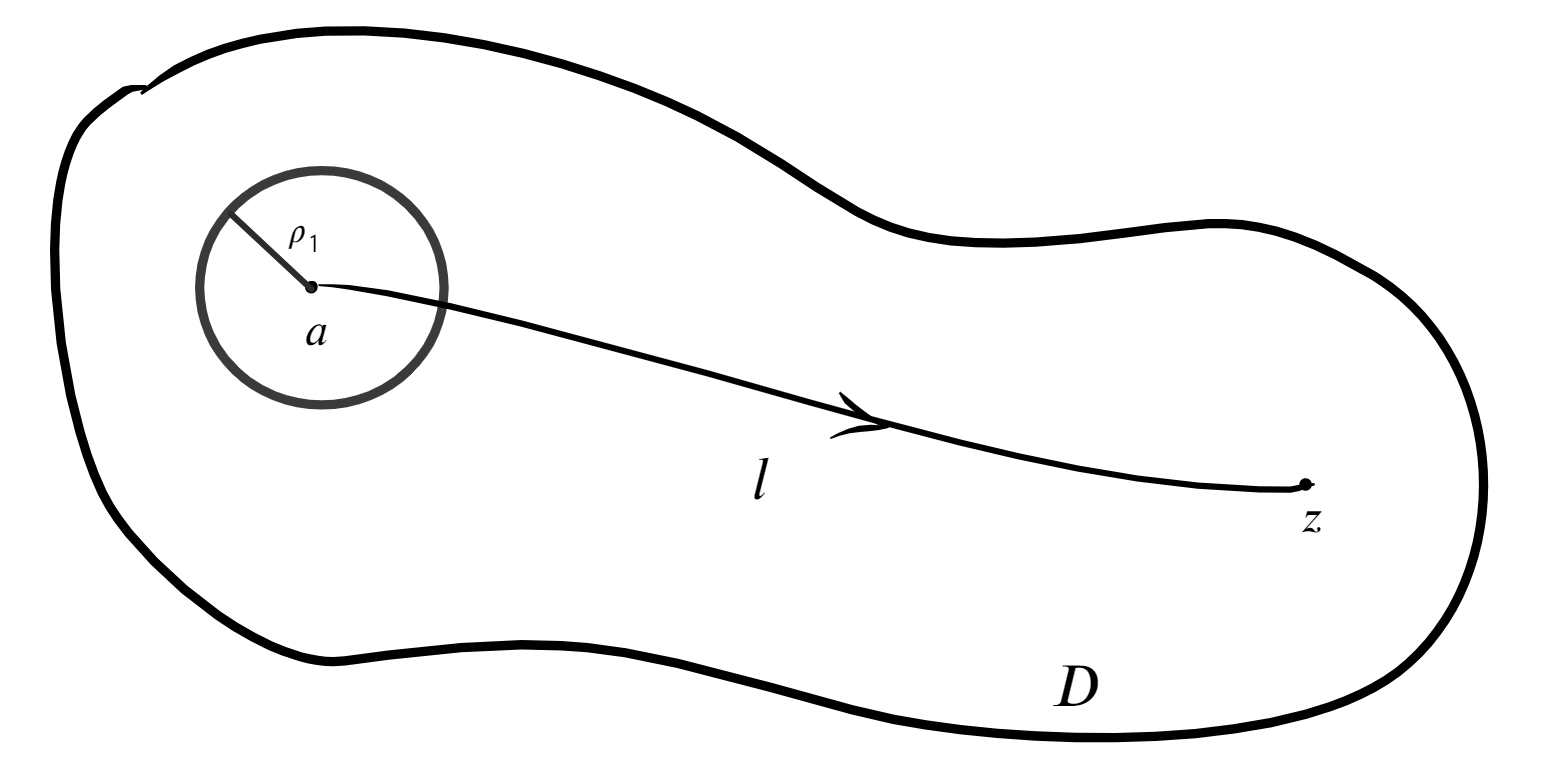
\includegraphics[scale=0.4]{images/036.png}$$
Покроем кривую $l$ конечным числом кругов радиуса $\rho$ с центрами в последовательных точках $z_1 = a$, $z_2$, $\ldots$, $z_n = z$. Таким образом, все круги лежат в области $D$, а центр каждого $j+1$-го круга лежит внутри $j$-го круга, $j = \overline{1,n-1}$.
$$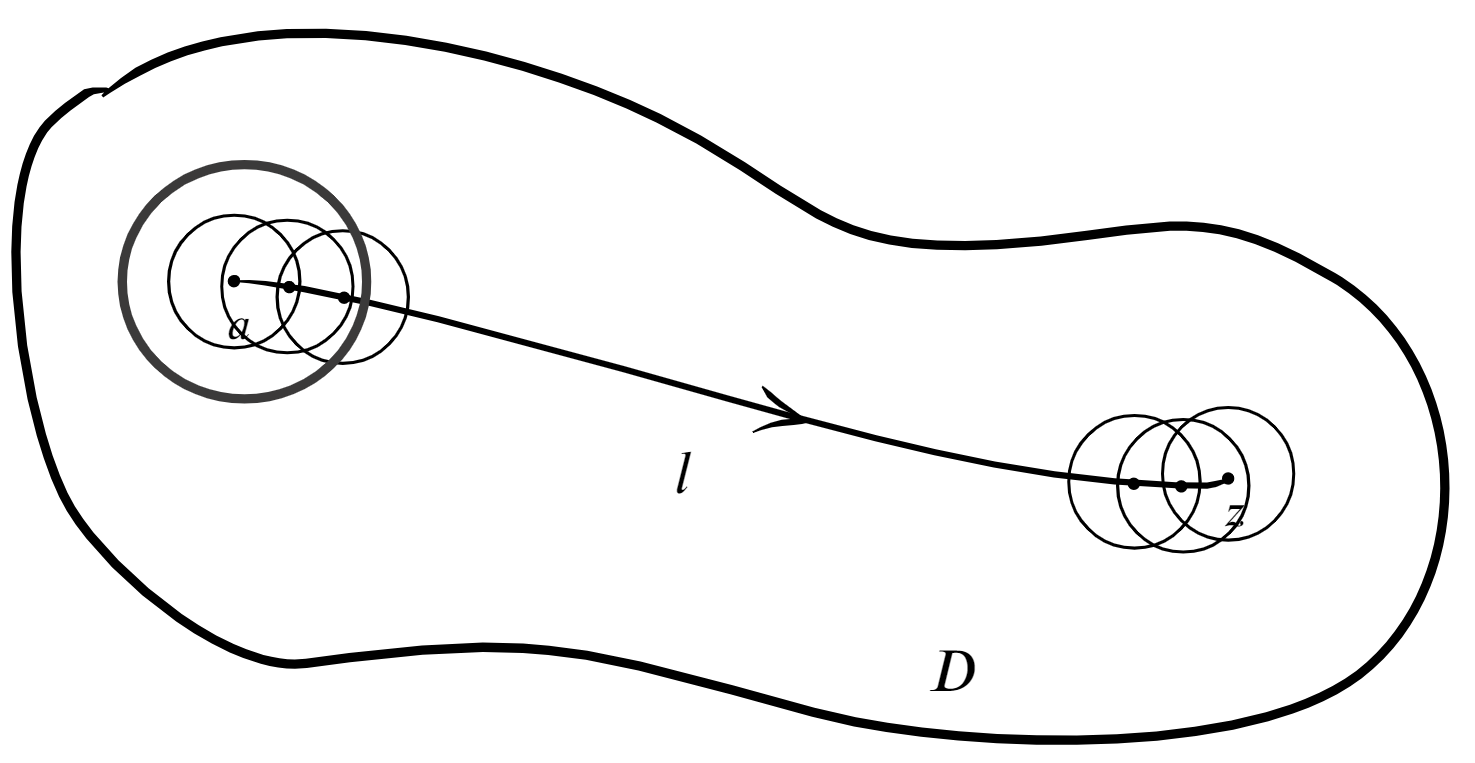
\includegraphics[scale=0.4]{images/037.png}$$
Так как $\rho_1 > \rho$, то круг радиуса $\rho_1$ с центром в $a$ содержит первый покрывающий круг. Следовательно, в первом круге $f(z) \equiv 0$ по ранее доказанной лемме. Аналогично во втором круге $f(z) \equiv 0$, поскольку центр второго круга лежит внутри первого. Продолжим эти рассуждения до тех пор, пока не придем к точке $z$. Тогда $f(z) \equiv0$ в области $D$.
\end{Proof}
\begin{cor}
	Пусть функции $f(z)$ и $g(z)$ регулярны в области $D$ и в точках последовательности $z_n$, $n = 1,2,\ldots$ функции $f$ и $g$ совпадают, то есть $f(z_n) = g(z_n)$, $\forall n$, и $z_n\underset{n\to \infty}{\longrightarrow} a \in D$. Тогда $f(z)\equiv g(z)$ в области $D$. 
\end{cor}\begin{Proof}
Рассмотрим функцию $h(z) = f(z) - g(z)$. Тогда $h(z_n) = 0$. По теореме единственности $h(z) \equiv 0$ в области $D$. Следовательно, функции $f(z)$ и $g(z)$ совпадают в области $D$.
\end{Proof}
\begin{cor}
	Если функции $f(z)$ и $g(z)$ регулярны в области $D$ и $f(z) = g(z)$ в некоторой подобласти $D_1$ области $D$ (или $f(z) = g(z)$ на некоторой гладной кривой из $D$), то $f(z) \equiv g(z)$ в области $D$.
\end{cor}
\section{Нули регулярной функции.}
Пусть функция $f(z)$ регулярна в области $D$.\\\\
$\bullet$ \textit{Если $f(z_0) = 0$, то точка $z_0$ называется \textbf{нулем функции}.}\\\\
Поскольку функция $f(z)$ регулярна, ее можно представить в виде $$f(z) = c_0 + c_1(z-z_0) + \ldots + c_n(z-z_0)^n + \ldots,\ |z-z_0|<\rho.$$
Отсюда $f(z_0) = c_0$. Из леммы к теореме единственности нули регулярной функции изолированы, то есть существует окрестность точки $z_0$, в которой $f(z_0) \equiv 0$ либо нет других нулей у функции. Пусть $c_n$ --- первый ненулевой коэффициент функции, то есть $c_0 = \ldots = c_{n-1} = 0$, $c_n \ne 0$. \\\\
$\bullet$ \textit{Индекс $n$ первого ненулевого коэффициента $c_n$ называется \textbf{порядком нуля}.}\\\\
Следовательно, $$f(z) = c_n(z-z_0)^n + c_{n+1}(z-z_0)^{n+1} + \ldots = (z-z_0)^n(c_n + c_{n+1}(z-z_0) + \ldots) = (z-z_0)^n h(z),$$
где $h(z)$ --- регулярная функция, причем $h(z_0)\ne 0$.
\begin{theorem}
	[первая теорема о порядке нуля]
	Точка $z_0$ --- нуль порядка $n$ $\Longleftrightarrow$ $f(z) = (z-z_0)^nh(z)$, $h(z_0) \ne 0$.
\end{theorem}\begin{theorem}
[вторая теорема о порядке нуля]
Число $n$ --- порядок нуля регулярной функции $\Longleftrightarrow$ $f^{(n)}(z_0)\ne 0$, $f^{(i)}(z_0) =0$, $\forall i = \overline{0,n-1}$. 
\end{theorem}
\section{Ряд Лорана.}
$\bullet$ \textit{\textbf{Рядом Лорана} называется ряд вида} $$\sum\limits_{n=-\infty}^{+\infty}c_n(z-z_0)^n = \ldots + c_{-n}(z-z_0)^{-n} + \ldots + c_{-1}(z-z_0)^{-1} + c_0 + c_1(z-z_0) + \ldots + c_n(z-z_0)^n + \ldots,\ c_i \in \Cm.$$
Обозначим $I_1 =\sum\limits_{n =-\infty}^{-1}c_n(z-z_0)^n $, $I_2 =\sum\limits_{n =0}^{\infty}c_n(z-z_0)^n$. Ряд $I_2$ является степенным рядом. А ряд $I_1$ сводится к степенному ряду с помощью замены $t = \dfrac{1}{z - z_0}$: $\sum\limits_{n =-\infty}^{-1}c_nt^{-n} = \sum\limits_{n =1}^{\infty}c_{-n}t^{n}.$\\\\
$\bullet$ \textit{Ряд Лорана называется \textbf{сходящимся}, если сходятся ряды $I_1$ и $I_2$.} \\\\
Ряд $I_2$ имеет область сходимости $|z-z_0|<R$, где $R$ --- радиус сходимости.\\\\
Ряд $I_1$ сводится к степенному ряду, который имеет радиус сходимости $\rho$. Тогда область сходимости ряда $I_1$ будет $\Big|\dfrac{1}{z-z_0}\Big|<\rho$. Отсюда $|z-z_0| > 1/\rho = r$. Тогда область сходимости ряда Лорана выглядит следующим образом:
$$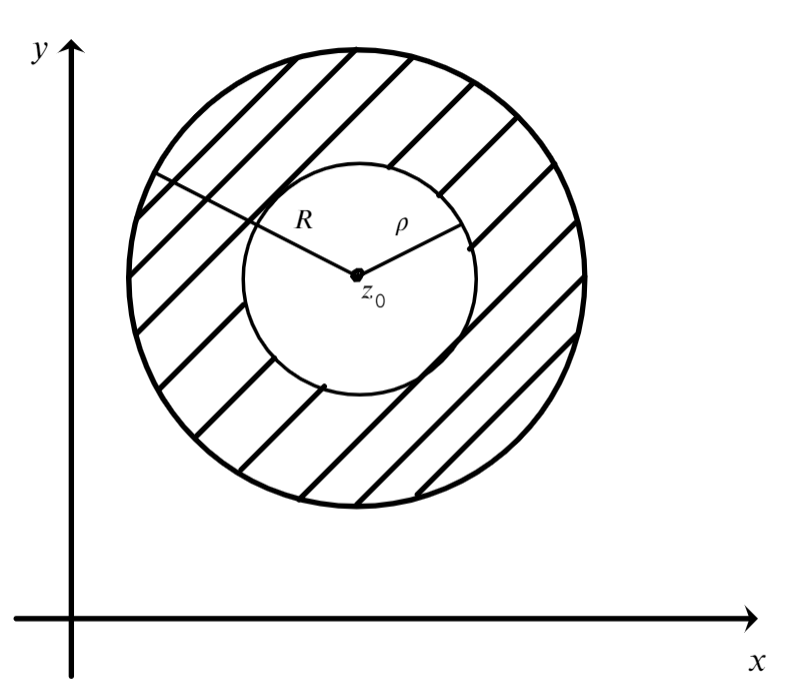
\includegraphics[scale=0.5]{images/040.png}$$
Если $r<R$, то область сходимости ряда Лорана --- кольцо $r < |z-z_0|<R$.\begin{theorem}
	[о представлении регулярной в кольце функции рядом Лорана]
	Если функция $f(z)$ регулярна в кольце $0\leq r < |z-z_0|<R$, то эта функция является суммой ряда Лорана, то есть $$f(z) = \sum\limits_{n=-\infty}^{+\infty}c_n(z-z_0)^n,$$ с коэффициентами $$c_n = \dfrac{1}{2\pi i}\int\limits_{C(z_0,\rho)}\dfrac{f(\zeta)}{(\zeta - z_0)^{n+1}}d\zeta,\quad r < \rho < R.$$
\end{theorem}\begin{Proof}
Обозначим через $K$ кольцо $r < |z-z_0| < R$. Рассмотрим кривые $\Gamma$ и $\gamma$, лежащие в кольце $K$. Возьмем произвольную точку $z\in K$, лежащую между кривыми $\Gamma$ и $\gamma$.
$$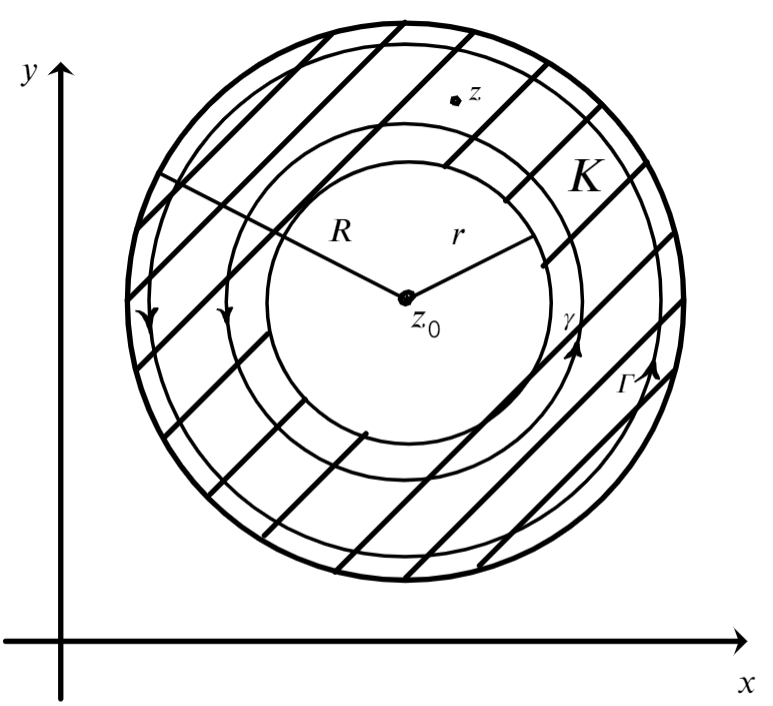
\includegraphics[scale=0.5]{images/041.png}$$
По следствию 1 из интегральной формулы Коши $$f(z) =\dfrac{1}{2\pi i} \int\limits_{\Gamma} \dfrac{f(\zeta)}{\zeta-z}d\zeta - \dfrac{1}{2\pi i}\int\limits_{\gamma}\dfrac{f(\zeta)}{\zeta-z}d\zeta.$$
Рассмотрим интеграл по $\Gamma$. По критерию регулярности $$\dfrac{1}{2\pi i} \int\limits_{\Gamma} \dfrac{f(\zeta)}{\zeta-z}d\zeta = \sumz c_n(z-z_0)^n.$$
Отсюда $$c_n = \dfrac{1}{2\pi i}\int\limits_{\Gamma}\dfrac{f(\zeta)}{(\zeta - z_0)^{n+1}}d\zeta.$$
Рассмотрим интеграл по $\gamma$. Разложим в степенной ряд функцию $-\dfrac{1}{\zeta - z}$ по степеням $z - z_0$: \begin{multline*}
	-\dfrac{1}{\zeta - z} = -\dfrac{1}{\zeta - z_0 + z_0 - z} =\dfrac{1}{(z-z_0) - (\zeta - z_0)}= \dfrac{1}{(z - z_0)(1 - \frac{\zeta-z_0}{z - z_0})}= \\=\sumz\dfrac{(\zeta-z_0)^n}{(z - z_0)^{n+1}} = [n+1 = -k] = \sum\limits_{k=-1}^{-\infty}\dfrac{(z-z_0)^k}{(\zeta - z_0)^{k+1}}.
\end{multline*}
Полученный ряд сходится равномерно на окружности $\gamma$ (это следует из леммы Абеля). Тогда ряд $$-\dfrac{f(\zeta)}{\zeta - z} = \sum\limits_{k=-1}^{-\infty}\dfrac{f(\zeta)}{(\zeta - z_0)^{k+1}}\cdot (z-z_0)^k$$
также сходится равномерно на окружности $\gamma$. А так как $\gamma$ --- это компакт и функция $f(\zeta)$ непрерывна на этом компакте, то функция $f(\zeta)$ ограничена. Почленно проинтегрируем этот ряд: $$-\dfrac{1}{2\pi i}\int\limits_\gamma \dfrac{f(\zeta)}{\zeta - z}d\zeta = \dfrac{1}{2\pi i}\sum\limits_{n=-1}^{-\infty}\Big(\int\limits_\gamma\dfrac{f(\zeta)}{(\zeta - z_0)^{n+1}}d\zeta \Big)\cdot (z-z_0)^n= \sum\limits_{n=-1}^{-\infty} c_n(z-z_0)^n,$$
где $$c_n = \dfrac{1}{2\pi i}\int\limits_\gamma  \dfrac{f(\zeta)}{(\zeta - z_0)^{n+1}}\cdot d\zeta.$$
Таким образом, ряд Лорана имеет вид $$f(z) = \sumz\Big( \dfrac{1}{2\pi i}\int\limits_{\Gamma}\dfrac{f(\zeta)}{(\zeta - z_0)^{n+1}}d\zeta\Big)(z-z_0)^n + \sum\limits_{n=-1}^{-\infty}\Big(\dfrac{1}{2\pi i}\int\limits_\gamma\dfrac{f(\zeta)}{(\zeta - z_0)^{n+1}}d\zeta \Big)\cdot (z-z_0)^n.$$
Возьмем окружность радиуса $\rho$. Обе кривые $\gamma$ и $\Gamma$ можно деформировать в эту окружность. Следовательно, вместо $\gamma$ и $\Gamma$ можно взять окружность радиуса $\rho$. 
$$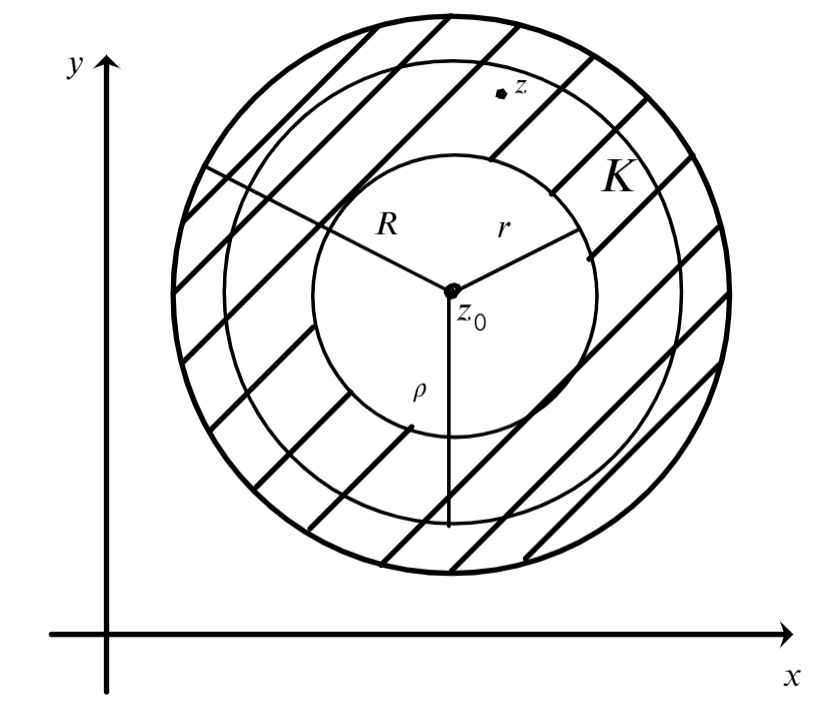
\includegraphics[scale = 0.5]{images/042.png}$$
Тогда ряд Лорана можно записать в виде $$f(z) = \sum\limits_{n=-\infty}^{+\infty}c_n(z-z_0)^n,$$ с коэффициентами $$c_n = \dfrac{1}{2\pi i}\int\limits_{C(z_0,\rho)}\dfrac{f(\zeta)}{(\zeta - z_0)^{n+1}}d\zeta.$$ 
\end{Proof}
\subsubsection*{Оценка для коэффициентов ряда Лорана.}
Пусть $M = \underset{z\in C(z_0,\rho)}{\max|f(z)|}$. Тогда $$|c_n| = \dfrac{1}{|2\pi i|}\cdot \Big|\int\limits_{C(z_0,\rho)}\dfrac{f(\zeta)}{(\zeta - z_0)^{n+1}}d\zeta \Big|\leq \dfrac{M}{2\pi}\int\limits_{C(z_0,\rho)}\dfrac{ds}{\rho^{n+1}} = \dfrac{M}{2\pi}\cdot \dfrac{ds}{\rho^{n+1}}\cdot 2\pi \rho = \dfrac{M}{\rho ^ n}, \forall n \in \Z.$$\begin{cor}
	[единственность разложения регулярной в кольце функции в ряд Лорана]
	Если функция $f(z)$ разложима в кольце $\rho < |z-z_0| < R$ в ряд Лорана, то это разложение единственно.
\end{cor}
\begin{Proof}
	От противного. Пусть существует 2 разложения в ряд Лорана: $$f(z) = \sumrl c_n(z-z_0)^n = \sumrl b_n(z-z_0)^n,\quad \rho < |z-z_0| < R.$$
	Домножим это уравнение на $(z-z_0)^{-m-1}$:
	$$\sumrl c_n(z-z_0)^{n-m-1} = \sumrl b_n(z-z_0)^{n-m-1}.$$
	Оба разложения сходятся равномерно на $C(z_0,R_0)$, $\rho < R_0<R$. Почленно проинтегрируем полученное равенство: $$\sumrl c_n \int\limits_{C(z_0,R_0)}(z-z_0)^{n-m-1}dz = \sumrl b_n \int\limits_{C(z_0,R_0)}(z-z_0)^{n-m-1}dz,$$
	$$\int\limits_{C(z_0,R_0)}(z-z_0)^{n-m-1}dz = \begin{cases}
		0,\ n-m-1 \ne -1,\\
		2\pi i,\ n-m-1 = -1.
	\end{cases}$$ 
Если $n-m-1 = -1$, то $n=m$, следовательно, $$\sumrl c_n\cdot 2\pi i = \sumrl b_n\cdot 2\pi i \Rightarrow c_n = b_n,\ \forall m \in \Z.$$ 
\end{Proof}
\section{Аналитическое продолжение.}
Пусть задана функция $f : E\to \Cm$, $E\subset D$, где $D$ --- произвольная область, и задана функция $F: D \to \Cm$.\\\\
$\bullet$ \textit{Функция $F(z)$ называется \textbf{аналитическим продолжением функции $f(z)$} из множества $E$ в область $D$, если $F(z) = f(z)$ $\forall z \in E$, а $F(z)$ --- регулярная в $D$ функция.}
\begin{theorem}
	[о единственности аналитического продолжения]
	Если множество $E$ содержит последовательность точек $z_n\underset{n\to \infty}{\longrightarrow} a \in E$, $z_i \ne z_j$ $\forall i,j$, $f(z)$ --- функция заданная на $E$ и $D$ --- область содержащая множество $E$, то существует единственное аналитическое продолжение функции $f(z)$ в области $D$.
\end{theorem}
\begin{Proof}
	Пусть существуют 2 аналитических продолжения функции $f(z)$ --- $F(z)$ и $G(z)$. Тогда $F(z_n) = G(z_n)$ $\forall n$ и  $z_n\underset{n\to \infty}{\longrightarrow} a \in E$, $z_i \ne z_j$ $\forall i,j$. Тогда из теоремы о единственности $F(z) = G(z)$ $\forall z \in D$.
\end{Proof}
\section{Особые точки.}
Пусть $B(z_0, R)$ --- круг $|z-z_0| < R$. Будем обозначать $$B^o(z_0, R)$$ --- \textbf{проколотая $R$-окрестность} точки $z_0$ (то есть круг $B(z_0, R)$ без точки $z_0$ или кольцо $0< |z-z_0|<R$).\\\\
$\bullet$ \textit{Точка $z_0$ называется \textbf{особой точкой} для функции $f(z)$, если $\exists B^o(z_0, \rho)$, $\rho > 0$, в которой функция $f(z)$ регулярная.}\\\\
По теореме о разложении регулярной функции в кольце функцию $f(z)$ можно представить в виде ряда Лорана $$f(z) = \ldots + c_{-n}(z-z_0)^{-n} + \ldots + c_{-1}(z-z_0)^{-1} + c_0 + c_1(z-z_0) + \ldots + c_n(z-z_0)^n + \ldots.$$
$\bullet$ \textit{Сумму $$\sum\limits_{n=-\infty}^{-1} = \ldots + c_{-n}(z-z_0)^{-n} + \ldots + c_{-1}(z-z_0)^{-1}$$ в разложении функции в ряд Лорана будем называть \textbf{главной частью ряда Лорана}, а сумму $$\sum\limits_{n=0}^{+\infty} = c_0 + c_1(z-z_0) + \ldots + c_n(z-z_0)^n + \ldots$$ --- \textbf{правильной частью ряда Лорана}.}\\\\
Будем различать 3 типа особых точек:\begin{enumerate}
	\item \textit{устранимая особая точка};
	\item \textit{полюс};
	\item \textit{существенно особая точка}.
\end{enumerate}
$\bullet$ \textit{Особая точка функции $f(z)$ называется \textbf{устранимой особой точкой}, если} $$\exists \lim\limits_{z\to z_0} f(z) = A\in \Cm.$$
$\bullet$ \textit{Особая точка функции $f(z)$ называется \textbf{полюсом}, если} $$\exists \lim\limits_{z\to z_0} f(z) = \infty.$$
$\bullet$ \textit{Особая точка функции $f(z)$ называется \textbf{существенно особой точкой}, если} $$\not\exists \lim\limits_{z\to z_0} f(z).$$
\begin{theorem}
	[об устранимой особой точке] Точка $z_0$ --- устранимая особая точка функции $f(z)$ $\Longleftrightarrow$ главная часть разложения функции в ряд Лорана тождественно равна нулю.
\end{theorem}\begin{Proof}
$\Rightarrow)$ Рассмотрим функцию $f(z)$ такую, что $z_0$ для нее --- устранимая особая точка. Докажем, что главная часть в разложении в ряд Лорана отсутствует. Берем ряд Лорана
$$f(z) = \ldots + c_{-n}(z-z_0)^{-n} + \ldots + c_{-1}(z-z_0)^{-1} + c_0 + c_1(z-z_0) + \ldots + c_n(z-z_0)^n + \ldots.$$
Точка $z_0$ --- устранимая особая точка, следовательно, $\exists \lim\limits_{z\to z_0} f(z) = A\in \Cm\Rightarrow$ функция $f(z)$ ограничена, то есть $\exists M : |f(z)|\leq M$ в круге $0 < |z-z_0| < \rho _1$. Воспользуемся неравенством для коэффициентов ряда Лорана:
$$|c_n|\leq \dfrac{M}{R_0^n},\ M = \underset{z \in C(z_0,\rho)}{\max} |f(z)|,$$
где $0 < R_0 < \rho_1$. Тогда $|c_{-n}| \leq MR_0^n$, но $R_0$ может быть сколь угодно близким к 0. Тогда, если $R_0\to 0$, то $MR_0^n \to 0$, следовательно, $c_{-n} = 0$, то есть все коэффициенты главной части ряда Лорана равны нулю, значит, главная часть равна нулю.\\\\
$\Leftarrow)$ Пусть главная часть разложения в ряд Лорана функции $f(z)$ отсутствует, то есть в круге $0 < |z-z_0|<\rho$ $$f(z) = c_0 + c_1(z-z_0) +\ldots + c_n(z-z_0)^n + \ldots.$$
Берем функцию $$g(z) = c_0 + c_1(z-z_0) +\ldots + c_n(z-z_0)^n + \ldots.$$ Тогда $f(z) = g(z)$ в кольце $0 < |z-z_0|<\rho$. И функция $g(z)$ определена и непрерывна в круге $|z-z_0| < \rho$ (в то время как $f(z)$ может быть и не определена). Следовательно, $$g(z_0) = A = \lim\limits_{z\to z_0} g(z) = \lim\limits_{z\to z_0}f(z).$$
\end{Proof}\\
\textbf{Замечание.} \textit{При доказательстве теоремы мы использовали ограниченность функции $f(z)$ в некоторой окрестности точки $z_0$. Поэтому теорема остается справедливой, если условие существования конечного предела заменить ограниченностью функции $f$ в окрестности точки $z_0$.}
\section{Полюсы, существенно особые точки.}
\begin{theorem}
	[Первая теорема о полюсе]
	Особая точка $z_0$ является полюсом функции $f(z)$ $\Longleftrightarrow$ функцию $f(z)$ можно представить в виде $$f(z) = \dfrac{h(z)}{(z-z_0)^m},$$ где $h(z)$ --- регулярная в окрестности точки $z_0$, $h(z_0) \ne 0$, $m \in \N$.
\end{theorem}\begin{Proof}
$\Rightarrow)$ Пусть функция $f(z)$ в точке $z_0$ имеет полюс, значит $\lim\limits_{z\to z_0} f(z) = \infty$.\\\\ Рассмотрим функцию $g(z) = \dfrac{1}{f(z)}$. Тогда существует окрестность точки $z_0$ такая, что $|f(z)| \geq 1$, $0<|z-z_0| < \rho_1$. Тогда в этой окрестности функция $g(z)$ ограничена и регулярна.\\\\
По замечанию из теоремы об устранимой особой точке $z_0$ --- устранимая особая точка, то есть $$\lim\limits_{z
\to z_0} g(z) = \lim\limits_{z
\to z_0} \dfrac{1}{f(z)} = 0.$$
Доопределим фунцию $g(z)$ в точке $z_0$: пусть $g(z_0) = 0$. Тогда получим фунцию, у которой точка $z_0$ является нулем. По одной из теорем о нулях функции функция $g(z)$ может быть представлена в виде $$g(z) = (z-z_0)^m\cdot h_1(z).$$
Причем функция $h_1(z)$ ругелярна в окрестности точки $z_0$ и $h_1(z_0) \ne 0$. Тогда $$f(z) = \dfrac{h(z)}{(z-z_0)^m},\ h(z) = \dfrac{1}{h_1(z)},$$
$\Leftarrow)$ Пусть функция $f(z)$ представима в виде $$f(z) = \dfrac{h(z)}{(z-z_0)^m}.$$
Тогда $\lim\limits_{z\to z_0} \dfrac{h(z)}{(z-z_0)^m} = \infty$, то есть точка $z_0$ --- полюс.
\end{Proof}\\\\
\textbf{Замечание.} \textit{Число $m$ из теоремы называется \textbf{порядком} полюса. Из доказательства следует, что порядок полюса равен порядку нуля функции $\dfrac{1}{f(z)}$.}
\begin{theorem}
	[Вторая теорема о полюсе]
	Точка $z_0$ является полюсом функции $f(z)$ $\Longleftrightarrow$ главная часть ряда Лорана в точке $z_0$ содержит конечное число слагаемых.
\end{theorem}
\begin{Proof}
	$\Rightarrow)$ Пусть точка $z_0$ --- полюс функции $f(z)$, а значит этот полюс имеет порядок. Пусть число $m$ --- порядок полюса. По первой теореме о полюсе $f(z)$ можно представить как $$f(z) = \dfrac{h(z)}{(z-z_0)^m},$$ где функция $h(z)$ регулярна в точке $z_0$ и $h(z_0)\ne0$. Тогда функцию $h(z)$ можно разложить в степенной ряд $$h(z) = c_0 + c_1(z-z_0) + \ldots = \sumz c_n(z-z_0)^n,\ |z-z_0| < \rho_2,\quad \rho_2 > 0.$$ Причем заметим, что $c_0 \ne 0$. Тогда $$f(z) = \dfrac{h(z)}{(z-z_0)^m} = \dfrac{c_0}{(z-z_0)^m} + \ldots + \dfrac{c_{m-1}}{z-z_0} + c_m + c_{m+1}(z-z_0) + \ldots \eqno (1)$$
	То есть в главной части разложения функции $f(z)$ в ряд Лорана конечное число слагаемых, а порядок полюса равен количеству слагаемых в главной части.\\\\
	$\Leftarrow)$ Пусть функция $f(z)$ имеет вид (1). Тогда вынесем за скобки множитель $\dfrac{1}{(z-z_0)^m}$:
	$$f(z) = \dfrac{1}{(z-z_0)^m} \cdot \underbrace{\Big(c_0 + \ldots + \dfrac{c_{m-1}}{(z-z_0)^{m-1} + \ldots}\Big)}_{h(z)},\quad h(z_0) = c_0 \ne 0.$$
	То есть функция $f(z)$ представима в виде $$f(z) = \dfrac{h(z)}{(z-z_0)^m}.$$ Тогда по первой теореме о полюсе точка $z_0$ --- полюс.
\end{Proof}\\\\
\textbf{Замечание.} \textit{Из первой теоремы о полюсе следует, что если точка $z_0$ является полюсом порядка $m$, то $$f(z)\underset{z\to z_0}{\sim}\dfrac{A}{(z-z_0)^m},\ A\ne 0,\ h(z_0) = A.$$}
\begin{theorem}
	[о существенно особой точке]
	Точка $z_0$ является существенно особой точкой функции $f(z)$ $\Longleftrightarrow$ главная часть разложения функции в ряд Лорана содержит бесконечное число слагаемых.
\end{theorem}\begin{Proof}
Вытекает из теоремы об устранимой особой точке и второй теоремы о полюсе.
\end{Proof}
\section{Особая точка $z = \infty$.}
Если функция $f(z)$ регулярна в кольце $R < |z| < \infty$, то бесконечность считается особой точкой. Для особой точки $z = \infty$ используются те же определения, то есть определяют устранимую особую точку, полюс и существенную особую точку.\\\\
Рассмотрим функцию $g(z) = f\Big(\dfrac{1}{z}\Big)$. Функция $g(z)$ будет регулярной в кольце $0< | z| <\dfrac{1}{R}$. Тогда для функции $g(z)$ особая точка $z = 0$. Отсюда следует разложение в ряд Лорана для функции $f(z)$ в окрестности бесконечности:
$$f(z) = \ldots + \dfrac{c_{-m}}{z^m} +\ldots + \dfrac{c_{-1}}{z} + c_0 + c_1z + \ldots + c_mz^m + \ldots,\quad R < |z| < \infty.$$
Заменим $t = \dfrac{1}{z}$ и заметим, что правильной частью является сумма $$\ldots + \dfrac{c_{-m}}{z^m} +\ldots + \dfrac{c_{-1}}{z} + c_0$$
а главной частью --- сумма $$c_1z + \ldots + c_mz^m + \ldots$$
То есть слагаемые, которые стремятся к бесконечности при стремелении $z$ к особой точке, образуют главную часть ряда Лорана.\begin{theorem}
	[об устранимой особой точке $z = \infty$] Точка $z = \infty$ --- устранимая особая точка функции $f(z)$ $\Longleftrightarrow$ главная часть разложения функции в ряд Лорана тождественно равна нулю.
\end{theorem}
\begin{theorem}
	[о полюсе $z = \infty$] Точка $z = \infty$ --- полюс порядка $m$ функции $f(z)$ $\Longleftrightarrow$ функция $f(z)$ представим в виде $$f(z) = z^m h(z),$$ где функция $h(z)$ регулярна в окрестности точки $z = \infty$ и $h(\infty) \ne 0$.
\end{theorem}
\begin{theorem}
	[о существенно особой точке $z = \infty$] Точка $z = \infty$ --- существенно особая точка функции $f(z)$ $\Longleftrightarrow$ в главной части разложения функции в ряд Лорана бесконечное число слагаемых.
\end{theorem}
\section{Основная теорема алгебры.}
$\bullet$ \textit{Функция $f(z)$ называется \textbf{целой}, если она регулярна на $\mathbb{C}$.}
\begin{theorem}
	[Лиувилля] Если функция $f(z)$ целая и $|f(z)| \leq M\cdot |z|^m$, $M = const$, $m = 0,1,2,\ldots$ в некотором кольце $R < |z| < \infty$, то все коэффициенты $c_n = 0$ при $n = m+1, m+2, \ldots$, где все $c_n$ --- коэффициенты разложения в ряд Лорана для функции $f(z)$.
\end{theorem}\begin{Proof}
Запишем неравенство для коэффициентов разложения в ряд Лорана:
$$|c_n|\leq \dfrac{\widetilde{M}}{R_0^n},\quad R< R_0,\quad \widetilde{M} = \underset{|z| = R_0}{\max}|f(z)| \leq MR_0^m.$$
Тогда $$|c_n| \leq \dfrac{M}{R_0^n}R_0^m = MR_0^{m-n}.$$
Если $n > m$, то $c_n = 0$.
\end{Proof}
\begin{cor}
	Если функция $f(z)$ целая, удовлетворяющая условиям теоремы Лиувилля, то функция $f(z)$ является полиномом
	$$f(z) = c_0 + c_1z + \ldots + c_nz^n.$$
\end{cor}
\begin{cor}
	Если функция $f(z)$ целая и она ограничена в кольце $R < |z| < \infty$, то функция $f(z) = const \forall z \in \Cm$.
\end{cor}
\begin{theorem}
	[основная теорема алгебры]
	Любой многочлен вида $$P(z) = a_nz^n + a_{n-1}z^{n-1} + \ldots + a_1z + a_0,\quad n \geq 1$$ имеет по крайней мере один корень.
\end{theorem}
\begin{Proof}
	От противного. Пусть многочлен $P(z)$ не имеет корней. Рассмотрим функцию $f(z) = \dfrac{1}{P(z)}$. Эта функция целая, следовательно $$\lim\limits_{z\to \infty}f(z) = 0\Rightarrow |f(z)|\leq M\quad \forall z \in B(0,R),\ R>0.$$
	По второму следствию $f(z) = A$, где $A$ --- постоянная. Следовательно, $P(z) = A_1$, где $A_1$ так же постоянная, что является противоречием с тем, что степень многочлена $P(z)$ ненулевая.
\end{Proof}
\section{Вычеты.}
Рассмотрим функцию $f(z)$, регулярную в кольце $0 < |z-z_0| < \rho$, $\rho > 0$. Тогда функция $f(z)$ в этом кольце разложима в ряд Лорана
$$\rl.$$
$\bullet$ \textit{Коэффициент $c_{-1}$ в разложении в ряд Лорана называется \textbf{вычетом} функции $f(z)$ и обозначается} $$c_{-1} = \underset{z = z_0}{\res}f(z).$$
Причем $$c_{n} = \dfrac{1}{2\pi i} \int\limits_{C(z_0, R)} \dfrac{f(\zeta)}{(\zeta-z_0)^n+1}d\zeta.$$
Но $n = -1$, следовательно, $$c_{-1} =  \dfrac{1}{2\pi i} \int\limits_{C(z_0, R)} f(z)dz.$$
Отсюда $$\int\limits_{C(z_0, R)} f(z)dz = 2\pi i \cdot \underset{z = z_0}{\res}f(z).$$
\textbf{Вычисление вычетов.}
\begin{enumerate}
	\item Если $z_0$ --- устранимая особая точка, то вычет функции равен нулю.
	\item Если $z_0$ --- существенно особая точка, то вычет можно найти лишь разложив функцию в ряд Лорана.
	\item Если $z_0$ --- полюс, то существуют формулы, позволяющие находить вычеты функции
	\begin{enumerate}
		\item Пусть $z_0$ --- полюс первого порядка (простой полюс).\\\\
		Разложение функции $f(z)$ в ряд Лорана имеет вид 
		$$f(z) =\dfrac{c_{-1}}{(z-z_0)} + c_0 + c_1(z-z_0) + \ldots + c_n(z-z_0)^n + \ldots$$
		Домножим уравнение на $(z-z_0)$, тогда
	$$(z-z_0)\cdot f(z) =c_{-1} + c_0(z-z_0) + c_1(z-z_0)^2 + \ldots + c_n(z-z_0)^{n+1} + \ldots$$
	Таким образом, $$c_{-1} = \lim\limits_{z\to z_0}(z-z_0)\cdot f(z) =\resf.$$
	В частном случае, если функция $f(z)$ представима в виде $f(z) = \dfrac{h(z)}{g(z)}$, где $h(z)$ и $g(z)$ --- регулярные в точке $z_0$ функции, $h(z_0) \ne 0$, $g(z_0) = 0$, $g'(z_0) \ne 0$. Тогда  $$\lim\limits_{z\to z_0} \dfrac{h(z)}{g(z) - g(z_0)}\cdot (z-z_0) = \lim\limits_{z\to z_0} \dfrac{h(z)}{\frac{g(z) - g(z_0)}{(z-z_0)}}= \dfrac{h(z_0)}{g'(z_0)} = \underset{z=z_0}{\res} \dfrac{h(z)}{g(z)}.$$
	\item Пусть $z_0$ --- полюс $k$-ого порядка. Тогда функцию $f(z)$ можно разложить в ряд Лоарана $$f(z) =  \dfrac{c_{-k}}{(z-z_0)^k} + \dfrac{c_{-k-1}}{(z-z_0)^{k-1}} +\ldots + \dfrac{c_{-1}}{(z-z_0)} + c_0 + c_1(z-z_0) + \ldots$$
	Домножим последнее уравнение на $(z-z_0)^k$ и получим $$(z-z_0)^kf(z) = c_{-k} + c_{-k+1}(z-z_0) + \ldots + c_{-1}(z-z_0)^{k-1} + c_0(z-z_0)^k + \ldots$$
	Вычислим $(k-1)$-ую производную от этого уравнения:
	$$\Big((z-z_0)^kf(z)\Big)^{(k-1)} = (k-1)!\cdot c_{-1} + \widetilde{c_0}(z-z_0) + \ldots$$
	Тогда $$\lim\limits_{z\to z_0}\dfrac{\Big((z-z_0)^kf(z)\Big)^{(k-1)} }{(k-1)!} = c_{-1} = \resf.$$
	\end{enumerate}
\end{enumerate}
\section{Вычет в точке $z=\infty$.}
Пусть функция $f(z)$ регулярна в кольце $R<|z|<\infty$. Тогда она разложима в ряд Лорана в этом кольце $$f(z) = \ldots + \dfrac{c_{-n}}{z^n} + \ldots + \dfrac{c_{-1}}{z} + c_0 + c_1z + \ldots + c_nz^n + \ldots.$$
$\bullet$ \textit{Коэффициент $-c_{-1}$ называется \textbf{вычетом функции $f(z)$ в точке $z = \infty$}, то есть} $$-c_{-1} = \underset{z = \infty}{\res}f(z).$$
Опять же $$c_{-1} = \dfrac{1}{2\pi i }\int\limits_{C(0, R_0)}f(z) dz.$$
Тогда $$\int\limits_{C(0, R_0)}f(z) dz = -2\pi i \resinf.$$
Возьмем противоположную ориентацию кривой интегрирования, тогда
$$\int\limits_{C^-(0, R_0)}f(z) dz = 2\pi i \resinf.$$
\subsubsection*{Вычисление вычетов.}
Если $z = \infty$ --- устранимая особая точка, то разложение в ряд Лорана функции $f(z)$ имеет вид $$f(z) = c_0 + \dfrac{c_{-1}}{z} + \ldots + \dfrac{c_{-n}}{z^n} + \ldots.$$
Рассмотрим случай, когда $\lim\limits_{z \to \infty} f(z) = 0$. В таком случае $$f(z) = \dfrac{c_{-1}}{z} + \ldots + \dfrac{c_{-n}}{z^n}.$$
Тогда $$f(z) \underset{z \to \infty}{\sim} \dfrac{c_{-k}}{z^k},\quad k \geq 1.$$
Если $k> 1$, то $c_{-1} = 0$ и, соответственно, $\resinf = 0$.\\
Если $k=1$, то $c_{-1}\ne 0$ и $\resinf = -c_{-1} = A_1$.\\\\ Следовательно, $$f(z)\underset{z \to \infty}{\sim} \dfrac{A}{z}.$$
\begin{theorem}
	[о сумме вычетов]
	Если функция $f(z)$ в расширенной комплексной плоскости имеет конечное число особых точек, то $$\sum\limits_k\underset{z_k}{\res}f(z) + \resinf = 0.$$
\end{theorem}\begin{Proof}
Берем окружность радиуса $R$ такую, что она содержит внутри все конечные особые точки. А каждая особая точка находится в окрестности внутри окружности.
$$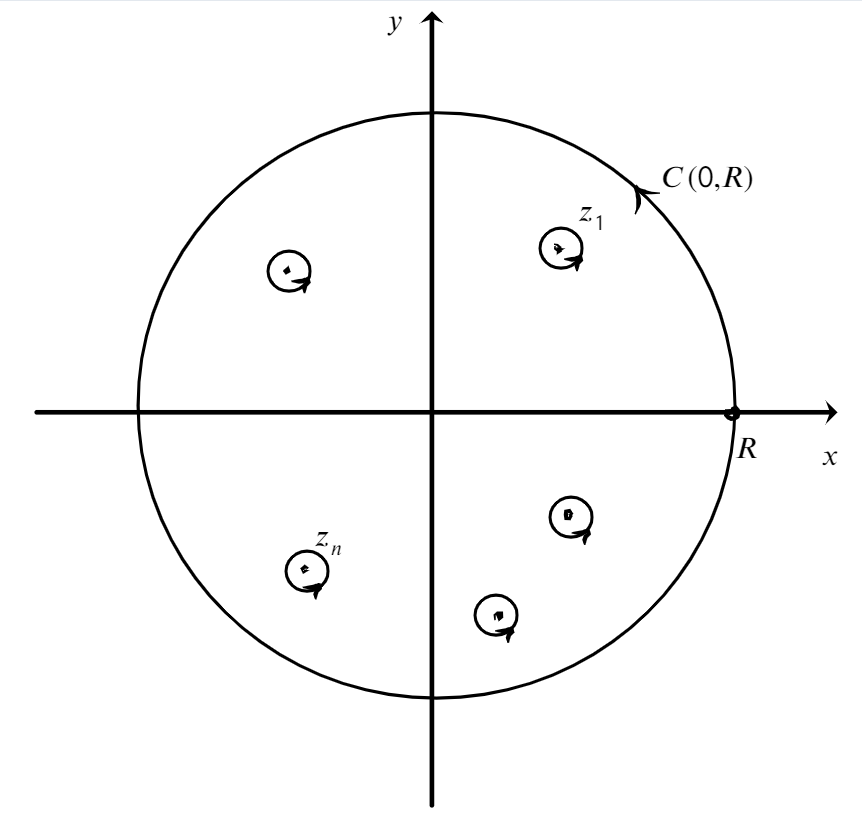
\includegraphics[scale=0.5]{images/043.png}$$
По следствию 3 из интегральной теоремы Коши $$\int\limits_{C(0,R)}f(z)dz = \sum\limits_k\int\limits_{C(z_k,R_k)}f(z)dz.$$
Причем $$-\resinf = \int\limits_{C(0,R)}f(z)dz = \sum\limits_k\int\limits_{C(z_k,R_k)}f(z)dz = \sum\limits_k\underset{z_k}{\res}f(z).$$
Получили искомое равенство.
\end{Proof}
\section{Основная теорема теории вычетов.}
\begin{theorem}
	[основная теорема теории вычетов]
	Если функция $f(z)$ регулярна в ограниченной области $D$ за исключением конечного числа особых точек, $\gamma$ --- простая замкнутая кусочно-гладкая кривая, лежащая в области $D$, не проходящая через особые точки, то $$\int\limits_\gamma f(z)dz = 2\pi i \sum\limits_{k=1}^n\underset{z_k}{\res}f(z),$$
	где $z_k$ --- все особые точки, лежащие внутри кривой $\gamma$.
	$$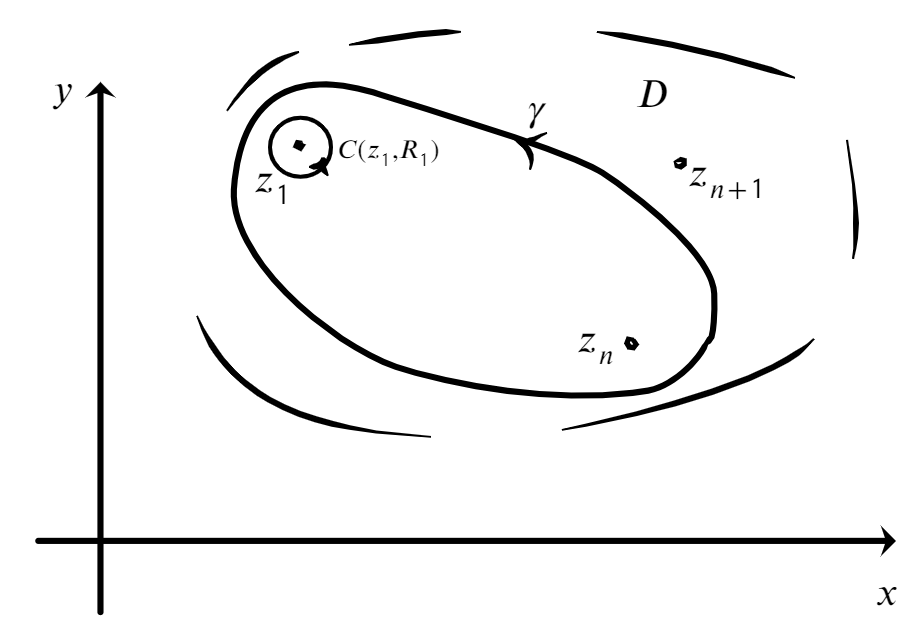
\includegraphics[scale=0.5]{images/044.png}$$
\end{theorem}\begin{Proof}
Возьмем окрестности особых точке $C(z_i, R_i)$. По следствию 3 из интегральной теоремы Коши $$\int\limits_\gamma f(z)dz = \sum\limits_{k=1}^n\int\limits_{C(z_k,R_k)}f(z)dz = 2\pi i \sum\limits_{k=1}^n\underset{z_k}{\res}f(z).$$
\end{Proof}
\section{Вычисление интегралов вида $\int\limits_0^{2\pi}R(\cos x,\sin x)dx$, $\int\limits_{-\infty}^{+\infty} R(x)dx$.}
\begin{enumerate}
	\item Рассмотрим интеграл вида $$\int\limits_0^{2\pi}R(\cos x,\sin x)dx,\eqno(1)$$ где $R$ --- рациональная функция двух переменных. Распишем $$\cos x = \dfrac{e^{ix} + e^{-ix}}{2},\quad \sin x = \dfrac{e^{ix} - e^{-ix}}{2i}.$$
	Если $z = e^{ix}$, то $dz = ie^{ix}dx$, отсюда $$dx = -i \dfrac{dz}{z}.$$
	Подставим полученные выражения и построим новый интеграл $$\int\limits_{|z| = 1}R\Big(\dfrac{z + 1/z}{2}, \dfrac{1 - 1/z}{2i}\Big)\Big(-i\dfrac{dz}{z}\Big) = \int\limits_{|z| = 1}R_1(z)dz,\eqno (2)$$
	где $R_1$ также рациональная функция.\\\\
	Вычисление интеграла (1) сводится к вычислению интеграла (2). Рациональная функция имеет конечное число особых точек и все они являются полюсом. Следовательно, к интегралу (2) применить основную теорему теории вычетов:
	$$\int\limits_{|z| = 1} R_1(z)dz = 2\pi i \sum\limits_{|z_i|<1} \res R_1(z).$$
	Тогда окончательно $$\int\limits_{0}^{2\pi} R(\cos x, \sin x)dx = 2\pi i \sum\limits_{|z_i|<1} \res R_1(z).$$
	\item Рассмотрим интеграл вида $$\int\limits_{-\infty}^{+\infty} R(x)dx.\eqno(3)$$
	Исследуем его на сходимость. Так как $R(x)$ --- рациональная функция, то она представима в виде частного неприводимых многочленов $$R(x) = \dfrac{P(x)}{Q(x)}.$$
	Если уравнение $Q(x) = 0$ имеет вещественный корень $x_0$, то интеграл $(3)$ является расходящимся, докажем это. Если $x_0$ --- вещественный корень кратности $m \geq 1$, то многочлен $Q(x)$ можно представить в виде $$Q(x) = (x-x_0)^m\cdot M(x),\quad M(x_0)\ne 0,\ P(x_0) \ne 0.$$
	В этом случае $$\dfrac{P(x)}{Q(x)} \underset{x\to x_0}{\sim} \dfrac{P(x_0)}{M(x_0)}\cdot \dfrac{1}{(x-x_0)^m}.$$
	Тогда, так как $m\geq 1$, то по степенному признаку сходимости интеграл $(3)$ является расходящимся.\\\\
	Таким образом, если есть корень у знаменателя, то интеграл $(3)$ расходится, следовательно, интеграл сходится если многочлен $Q(x)$ не обращается в нуль. \\\\Рассмотрим точку $x = \infty$. В таком случае $$\dfrac{P(x)}{Q(x)}\underset{x\to \infty}{\sim} \dfrac{x^n\cdot a_n}{x^m\cdot b_m} = \dfrac{M}{x^{m-n}}.$$
	Интеграл $(3)$ будет являться сходящимся, если $m-n > 1$, то есть $m > n+1$. А это значит, что $$\deg Q(x)\geq \deg P(x) + 2.$$
	Иначе интеграл $(3)$ будет расходящимся.\\\\
	Таким образом, интеграл $(3)$ является сходящимся, если многочлен $Q(x)$ не имеет вещественных корней и степень знаменателя функции $R(x)$ по крайней мере больше на 2 единицы степени числителя.
	\begin{lem}
		Если функция $f(z)$ регулярна в области, содержащей верхнюю полуплоскость, то есть $\Im z > 0$ за исключением конечного числа точек, не лежащих на вещественной оси и $$\int\limits_{C_R} f(z)dz \underset{R\to \infty}{\longrightarrow} 0,$$
		где $C_R$ --- полуокружность $|z| = R$, $\Im z > 0$: $$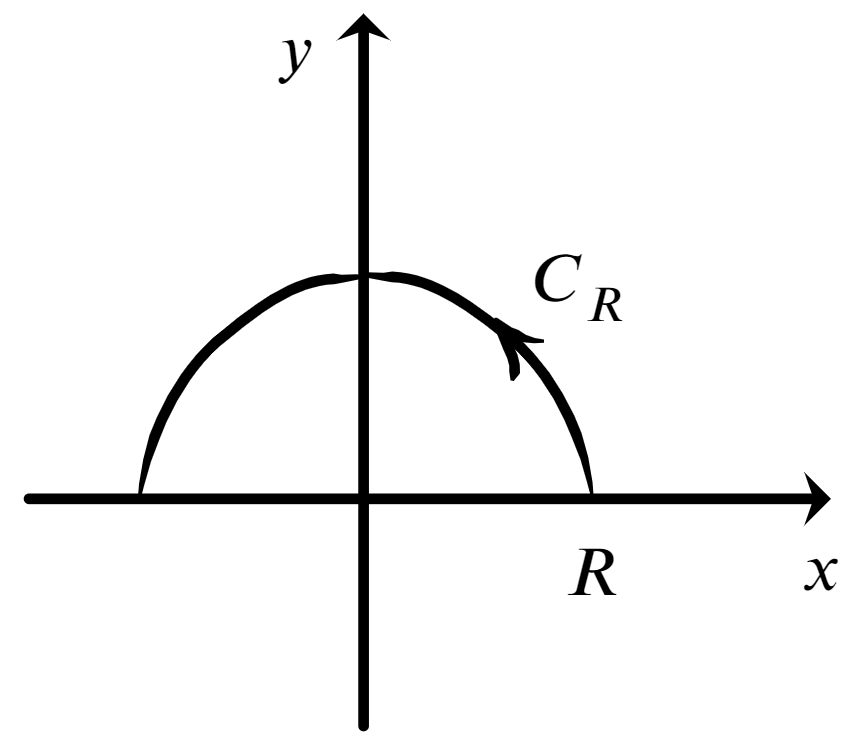
\includegraphics[scale=0.3]{images/045.png}$$
		то $$\int\limits_{-\infty}^{+\infty} f(x)dx = 2\pi i \sum\limits_{\Im z_i > 0} \underset{z_i}{\res}f(z).$$
		Предполагаем, что интеграл $\int\limits_{-\infty}^{+\infty} f(x)dx$ является сходящимся.
	\end{lem}
	\begin{Proof}
		Возьмем полуокружность $C_R$ таким образом, чтобы все особые точки, лежащие в верхней полуплоскости, попали в эту полуокружность. Пусть $\Gamma_R$ --- кривая, образованная полуокружностью и полуотрезком $(-R; R)$.
		$$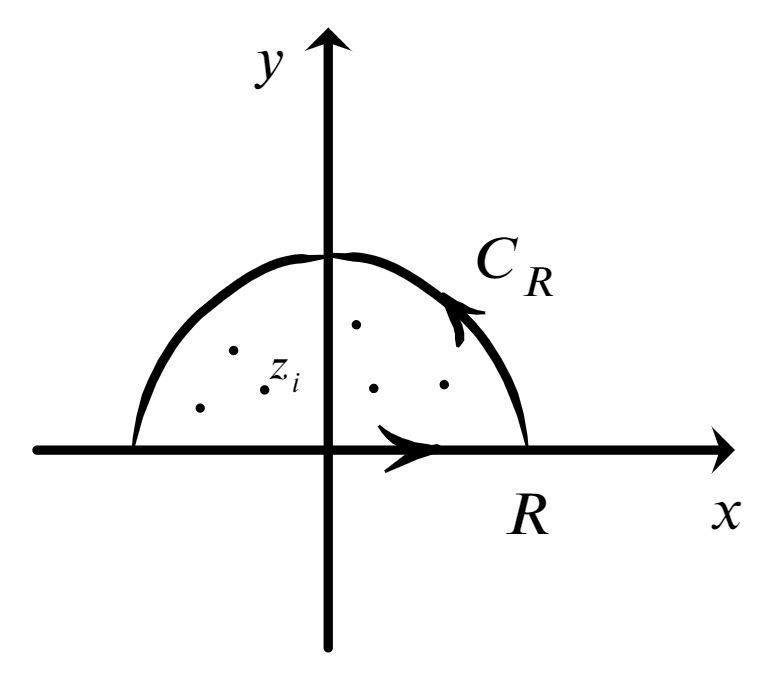
\includegraphics[scale=0.5]{images/046.png}$$
		По основной теореме вычетов $$\int\limits_{\Gamma_R} f(z)dz = 2\pi i \sum\limits_{\Im z_i > 0} \underset{z_i}{\res}f(z).$$
		Но, с другой стороны, $$\int\limits_{\Gamma_R} f(z)dz = \int\limits_{C_R} f(z)dz + \int\limits_{-R}^R f(x)dx.$$
		Устремим $R \to \infty$ и получим, что $$\int\limits_{C_R} f(z)dz \underset{R\to \infty}{\longrightarrow} 0,\quad \int\limits_{-R}^R f(x)dx \underset{R\to \infty}{\longrightarrow} \int\limits_{-\infty}^{+\infty} f(x)dx.$$
		Отсюда $$\int\limits_{-\infty}^{+\infty} f(x)dx = 2\pi i \sum\limits_{\Im z_i > 0} \underset{z_i}{\res}f(z).$$
	\end{Proof}\\
	Пусть интеграл (3) является сходящимся. Тогда функция $R(z)$ не имеет особых точек на вещественной оси и $$\lim\limits_{R\to +\infty} \int\limits_{C_R} R(z)dz = 0.$$
	Проверим это:
	$$\Big|\int\limits_{C_R} R(z)dz \Big|\leq \underset{z \in C_R}{\max}|R(z)|\cdot \pi R = \underset{z \in C_R}{\max} \Big| \dfrac{P(z)}{Q(z)}\Big|\cdot \pi R \leq \dfrac{M}{R^2}\cdot \pi R = \dfrac{M\pi}{R}\underset{R\to \infty}{\longrightarrow} 0.$$
	Все условия леммы выполнены, следовательно по лемме $$\int\limits_{-\infty}^{+\infty} R(x)dx = 2\pi i \sum\limits_{\Im z_i > 0} \underset{z_i}{\res}R(z).$$
\end{enumerate}
\section{Вычисление интегралов вида $\int\limits_{-\infty}^{+\infty} R(x)\cdot e^{i\alpha x}dx, \alpha > 0$.}
Рассмотрим интеграл вида $$\int\limits_{-\infty}^{+\infty} R(x)\cdot e^{i\alpha x}dx, \alpha > 0.\eqno (1)$$
Пусть $R(x) = \dfrac{P(x)}{Q(x)}$ --- рациональная функция и пусть $x_0$ --- корень знаменателя, то есть $Q(x_0) = 0$. Тогда $$\dfrac{P(x)}{Q(x)} \underset{x\to x_0}{\sim} \dfrac{M}{(x-x_0)^\alpha},\quad \alpha \geq 1.$$
Следовательно, интеграл (1) расходится по степенному признаку сходимости.
\\\\
Запишем интеграл (1) в виде $$\int\limits_{-\infty}^{+\infty} \dfrac{P(x)}{Q(x)}\cdot (\cos (\alpha x) + i\sin (\alpha x))dx, \alpha > 0.$$ Возьмем точку $x = +\infty$. По признаку Дирихле $$\Big|\int\cos xdx\Big| = \Big|\dfrac{1}{\alpha}\sin (\alpha x)\Big| \leq \dfrac{1}{\alpha}.$$
$$\Big|\int\sin xdx\Big|\leq \dfrac{1}{\alpha}.$$
При этом $$\dfrac{P(x)}{Q(x)}\underset{x\to 0}{\longrightarrow} 0$$ монотонно, когда $\deg P(x) + 1 \leq \deg Q(x)$.\\\\
Следовательно, интеграл (1) сходится $\Longleftrightarrow$ многочлен $Q(x)$ не имеет вещественных корней и $\deg Q(x) \geq \deg P(x ) + 1$.
\begin{lem}
	Если функция $g(z)$ непрерывна в области $|z| \geq R$,  $\Im z \geq 0$ и величина $$M(R) = \underset{z \in C_R}{\max}|g(z)|\underset{R\to \infty}{\longrightarrow} 0, $$
	то $$\int\limits_{C_R} g(z)\cdot e^{i\alpha z}dz \underset{R\to \infty}{\longrightarrow} 0.$$
\end{lem}\begin{Proof}
Без доказательства.
\end{Proof}\\\\
\textbf{Вычисление интеграла.}\\\\
Возьмем функцию $$g(z) = R(z)\cdot e^{i\alpha z}$$
 и пусть интеграл (1) сходится. Значит на вещественной оси у функции $g(z)$ нет особых точек. Тогда функция $g(z)$ удовлетворяет условиями леммы, а $$M(R) = \underset{z \in C_R}{\max} |R(z)|\cdot |e^{i\alpha z}| \leq \dfrac{M}{R}\underset{R\to \infty}{\longrightarrow} 0.$$
 Берем полуокружность $C_R$ и дополним ее полуотрезком $(-R; R)$
 $$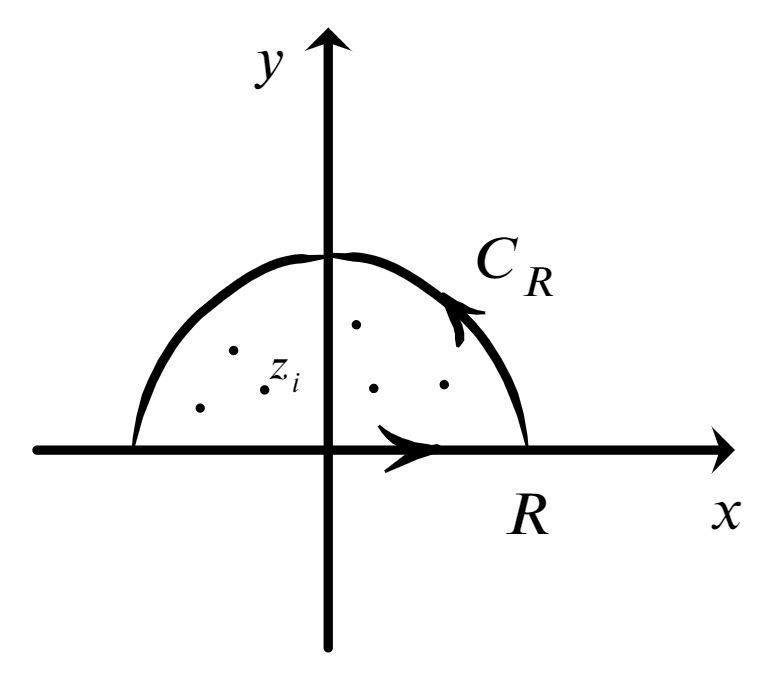
\includegraphics[scale=0.5]{images/046.png}$$
 Тогда $$\int\limits_{\Gamma_R} R(z)\cdot e^{i\alpha z}dz = 2\pi i \sum\limits_{\Im z_i > 0} \underset{z_i}{\res} R(z)\cdot e^{i\alpha z}dz.$$ 
 Причем, с другой стороны, $$\int\limits_{\Gamma_R} R(z)\cdot e^{i\alpha z}dz = \int\limits_{C_R}R(z)\cdot e^{i\alpha z}dz + \int\limits_{-R}^R R(x)\cdot e^{i\alpha x}dx.$$
 Тогда при $R \to \infty$ по лемме из предыдущего пункта $$\int\limits_{C_R}R(z)\cdot e^{i\alpha z}dz\underset{R\to \infty}{\longrightarrow} 0,\quad \int\limits_{-R}^R R(x)\cdot e^{i\alpha x}dx \underset{R\to \infty}{\longrightarrow} \int\limits_{-\infty}^{+\infty} R(x)\cdot e^{i\alpha x}dx.$$
 Следовательно, получаем $$\int\limits_{-\infty}^{+\infty} R(x)\cdot e^{i\alpha x}dx = 2\pi i \sum\limits_{\Im z_i > 0} \underset{z_i}{\res} R(z)\cdot e^{i\alpha z},\quad \alpha > 0.$$
 Поскольку $e^{i\alpha x} = \cos(\alpha x) + i\sin (\alpha x)$, то $$\int\limits_{-\infty}^{+\infty} R(x)\cdot \cos (\alpha x)dx = \Re \Big(2\pi i \sum\limits_{\Im z_i > 0} \underset{z_i}{\res} R(z)\cdot e^{i\alpha z}\Big),$$
 $$\int\limits_{-\infty}^{+\infty} R(x)\cdot \sin (\alpha x)dx = \Re \Big(2\pi \sum\limits_{\Im z_i > 0} \underset{z_i}{\res} R(z)\cdot e^{i\alpha z}\Big).$$
 \section{Оригиналы и изображеня. Преобразование Лапласа.}
 $\bullet$ \textit{Функция $f:(-\infty; + \infty) \to \Rm$ называется \textbf{оригиналом}, если она удовлетворяет следующим условиям:}\begin{enumerate}
 	\item \textit{$f(t)\equiv 0$ $\forall t < 0$;}
 	\item \textit{функция $f(t)$ кусочно-непрервная на интервале $(-\infty;+\infty)$;}
 	\item $\exists M = const$, $a = const$ : $$|f(t)|\leq Me^{at}\quad \forall t \in (-\infty; + \infty).$$
 	\textit{(то есть если функция возрастает, то возрастает не быстрее, чем некоторая эскпонента).}
 \end{enumerate}
Пусть $$L = \{a : |f(t)| \leq Me^{at},\ M=const\}.$$
$\bullet$ \textit{Число $a_0 = \inf\{L\}$ называется \textbf{показателем} роста функции $f(t)$.}\\\\
Если число $a_0$ --- показатель роста функции $f(t)$, то $$|f(t)| \leq Me^{(a_0 + \delta)t},\quad \forall\delta > 0.$$
Рассмотрим единичную функцию (функцию Хевисайда) $$1(t) = \begin{cases}
	0,\ t < 0,\\
	1,\ t \geq 0.
\end{cases}$$
Эта функция является оригиналом. Если функция $f(t)$ удовлетворяет второму и третьему условиям, но не удовлетворяет первому условию, то можно рассматривать функцию $f(t)\cdot 1(t)$. Такая функция будет являться оригиналом.\\\\
$\bullet$ \textit{Отображение, которое каждому оригиналу $f(t)$ ставит в соответствие функцию комплексного переменного $$F(p) = \int\limits_0^{+\infty}e^{-pt}f(t)dt,\quad p \in \Cm\eqno (1)$$ называется \textbf{преобразованием Лапласа}. Будем обозначать $f(t) \fallingdotseq F(p)$.}\\\\
$\bullet$ \textit{Функция $F(p)$ называется \textbf{изображением оригинала} $f(t)$.}\\\\
Функция $F(p)$ имеет особую точку $+\infty$.
\begin{theorem}
	[о множестве задания изображения]
	Если функция $f(t)$ --- оригинал c показателем роста $a_0$, то функция $F(p)$ определена в полуплоскости $\Re p > a_0$, причем интеграл $(1)$ сходится равномерно в полуплоскости $\Re p \geq \beta > a_0$. И изображение обладает свойством $$|F(p)|\underset{\Re p \to \infty}{\longrightarrow}0.$$
	$$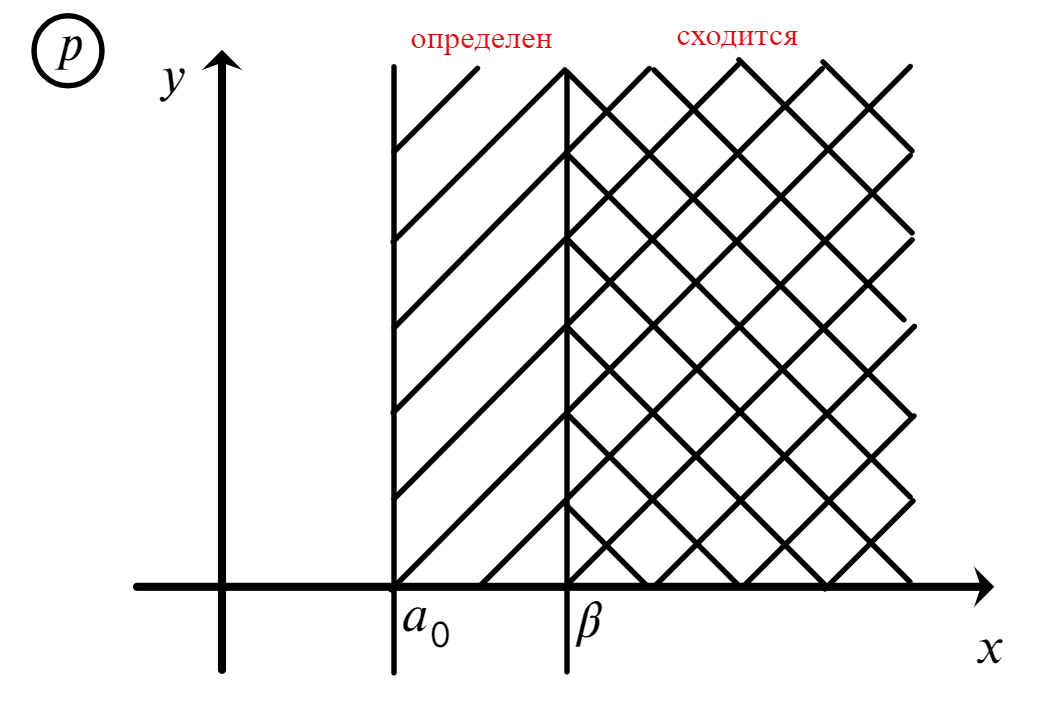
\includegraphics[scale=0.4]{images/047.png}$$
\end{theorem}\begin{Proof}
Возьмем число $p \in \Cm$ такое, что $\Re p > a_0$. Тогда $$\exists \epsilon > 0 : \Re p > a_0 + \epsilon.$$
Следовательно, $$|e^{-pt}f(t)| \leq \Big[|e^{-pt}| = |e^{(-x-iy)t}| = e^{-xt}\Big]\leq Me^{(a_0 + \epsilon)t}\cdot e^{-xt},\quad \Re p = x > a_0 + \epsilon.$$
Следовательно, $$M\cdot \int\limits_0^{+\infty}e^{(a_0 + \epsilon)t}dt = \dfrac{M\cdot e^{(a_0 + \epsilon)t}}{a_0 + \epsilon -x}\Big|_0^{+\infty} = -\dfrac{M}{a + \epsilon - x}.$$
Следовательно, интеграл (1) сходится. Тогда $\Re p > a_0$. А из последнего равенства вытекает $|F(p)|\underset{\Re p \to \infty}{\longrightarrow}0.$\\\\
Докажем равномерную сходимость. Пусть $\Re p \geq \beta > a_0$. Тогда $$|f(t)\cdot e^{-pt}| \leq e^{-\beta t}\cdot M \cdot e^{(a_0 + \epsilon)t}.$$
Выражение справа в последнем неравенстве --- мажоранта. Возьмем $\epsilon$ такое, что $-\beta + a_0 + \epsilon < 0$. Следовательно, мажоранта сходится. Отсюда по признаку Вейрштрасса исходный интеграл (1) сходится равномерно в полуплоскости $\Re p \geq \beta > a_0.$
\end{Proof}
\section{Теорема о регулярности преобразования Лапласа.}
\begin{theorem}
	[Морера]
	Если функция $f(z)$ непрерывна в области $D$ и интеграл по любой замкнутой кусочно-гладкой кривой $\gamma$ равен нулю, т. е. $$\int\limits_\gamma f(z)dz = 0,$$
	то функция $f(z)$ регулярна в области $D$.
\end{theorem}
\begin{Proof}
	Первая часть теоремы доказывается аналогично теореме о первообразной. То есть $$F'(z) = f(z)\quad \forall z \in D.$$
	Тогда функция $f(z)$ также регулярна в $D$, следовательно, она регулярна в $D$.
\end{Proof}\\\\
Если существует непрерывная функция $z = z(t)$, причем $t \in I = (-\infty; \beta)$ (или $I = (\alpha; +\infty)$, или $I = (-\infty; + \infty)$), то эта функция задает \textbf{неограниченную кривую} $\gamma$. Иначе, если $z =z(t)$, $t\in [\alpha; \beta]$, то кривая $\gamma$ \textbf{ограниченная}.
\begin{theorem}
	[о регулярности ИЗОП]
	Рассмотрим Ф2П $f(z,\zeta)$, $z \in D$ --- область, $\zeta \in \gamma$ --- некоторая кривая. Если выполняются условия:\begin{enumerate}
		\item функция $f(z,\zeta)$ непрерывна как Ф2П на множестве пар $(z,\zeta)\in D \times \gamma$, где $\gamma$ --- ограниченная кривая;
		\item при каждом $\zeta \in \gamma$ функция $f(z, \zeta)$ регулярна в области $D$,
	\end{enumerate}
	то функция $$F(z) = \int\limits_\gamma f(z,\zeta)d\zeta$$ регулярная в $D$.
\end{theorem}\begin{Proof}
Возьмем произвольную точку $z_0$ в области $D$ и круг с центром в этой точке, принадлежащий области $D$. Берем любую замкнутую кривую $\gamma_1$, лежащую в этом круге.
$$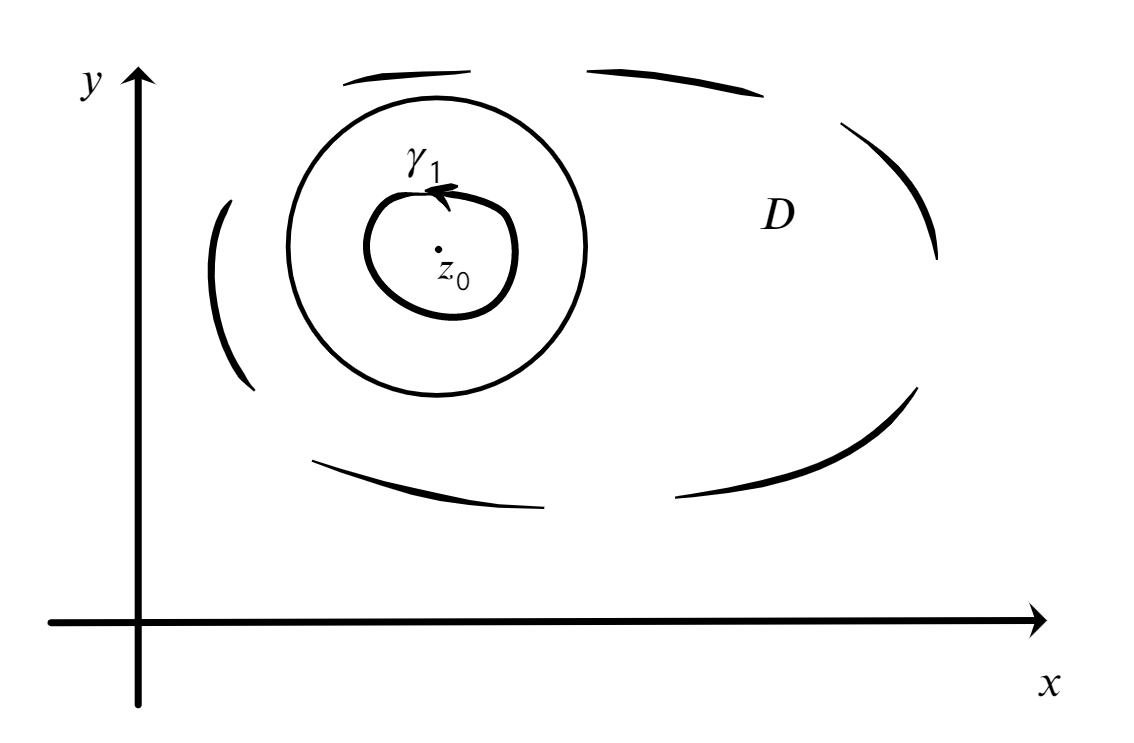
\includegraphics[scale=0.4]{images/048.png}$$
Рассмотрим интеграл $$\int\limits_{\gamma_1}F(z)dz = \int\limits_{\gamma_1}\Big(\int\limits_{\gamma}f(z,\zeta)d\zeta\Big)dz = \int\limits_\gamma \Big(\int\limits_{\gamma_1}f(z,\zeta)dz\Big)d\zeta = 0.$$
Тогда функция $F(z)$ регулярна в области $D$ по теореме Морера.
\end{Proof}
\begin{cor}
	Пусть выполняются условия теоремы кроме предположения о том, что $\gamma$ --- конечная кривая, то есть $\gamma$ --- бесконечная кривая, и выполняется улосвие \begin{enumerate}
		\item [3.] интеграл $\int\limits_\gamma f(z,\zeta)d\zeta$ сходится равномерно по $z \in K$, где $K$ --- любая замкнутая области из $D$. 
	\end{enumerate}
	Тогда функция $$F(z) = \int\limits_\gamma f(z,\zeta)d\zeta$$ регулярна в $D$.
\end{cor}
\begin{theorem}
	[о регулярности преобразования Лапласа]
	Функция $$F(p) = \int\limits_0^{+\infty}e^{-pt}f(t)dt,$$ если $f(t)$ --- оригинал, регулярна в области $\Re p > a_0$.
\end{theorem}\begin{Proof}
Доказательство вытекает из последнего следствия. Применим следствие к функции $f(z,t) = e^{-pt}f(t)$. Условие 3 вытекает из теоремы о множестве задания преобразования Лапласа. Следовательно, функция $F(p)$ регулярна в области $\Re p > a_0$.
\end{Proof}
\section{Свойства преобразования Лапласа.}
\begin{enumerate}
	\item \textbf{Линейность.} \textit{Если $f(t) \fallingdotseq F(p)$, $g(t)\fallingdotseq G(p)$, то} $$\alpha f(t) + \beta g(t) \fallingdotseq \alpha F(p) + \beta G(t),\quad \alpha, \beta \in \Cm.$$
	\begin{Proof}
		$$\int\limits_0^{+\infty}(\alpha f + \beta g) e^{-pt} dt = \alpha \int\limits_0^{+\infty}f(t)e^{-pt}dt + \beta \int\limits_0^{+\infty}g(t)e^{-pt}dt = \alpha F(p) + \beta G(p),\quad \alpha, \beta \in \Cm.$$
	\end{Proof}
	\item \textbf{Подобие.} \textit{Если $f(t)\fallingdotseq F(p)$, то $$f(at) \fallingdotseq \dfrac{1}{a}F\Big(\dfrac{p}{a}\Big),\quad a \in \Rm, a > 0.$$}
	\begin{Proof}
		$$\int\limits_0^{+\infty}f(at)e^{-pt}dt = \Big[at = s,\ dt = \dfrac{ds}{a}\Big] = \dfrac{1}{a} \int\limits_0^{+\infty} f(s)e^{-\frac{ps}{a}}ds = \dfrac{1}{a}F\Big(\dfrac{p}{a}\Big),\quad a \in \Rm, a > 0.$$
	\end{Proof}
	\item \textbf{Преобразование Лапласа для экспоненты и степенной функции.} \begin{enumerate}
		\item $e^t \fallingdotseq F(p-1)$;
		\begin{Proof}
			$$\int\limits_0^{+\infty}e^t \cdot e^{-pt}dt = \int\limits_0^{+\infty} e^{-(p-1)t} dt = F(p-1).$$
		\end{Proof}
		\item $t^\alpha \fallingdotseq \dfrac{\Gamma(\alpha + 1)}{p^{\alpha + 1}}.$
		\begin{Proof}
			Обозначим $F(p) = \int\limits_0^{+\infty}t^\alpha e^{-pt} dt$, $\Re p > 0$. И пусть $p = x \in \mathbb{R}$. Тогда $$\int\limits_0^{+\infty} t^\alpha \cdot  e^{-xt}dt = \Big[xt = s,\ t = \dfrac{s}{x},\ dt = \dfrac{ds}{x}\Big] = \dfrac{1}{x^{\alpha + 1}}\int\limits_0^{+\infty} e^{-s}\cdot s^{\alpha} ds = \dfrac{1}{x^{\alpha + 1}}\cdot \Gamma(\alpha + 1).$$ $$\Big(\text{так как }\Gamma(a) = \int\limits_0^{+\infty} e^{-t}\cdot t^{a-1}dt\Big)$$
			Функция $F(p)$ регулярна в полуплоскости $\Re p > 0$. При $ p = x$ она будет совпадать с $F(x)$, то есть $F( p ) = F(x)$. По теореме единственности существует единственное аналитическое представление регулярной функции. Тогда $$t^\alpha \fallingdotseq \dfrac{\Gamma(\alpha + 1)}{p^{\alpha + 1}}.$$ 
		\end{Proof}\\
		\textit{Если $\alpha = n \in \N$, то $$t^n  \fallingdotseq \dfrac{\Gamma(n + 1)}{p^{n + 1}} = \dfrac{n!}{p^{n+1}}.$$}
	\end{enumerate}
		\item \textbf{Дифференцирование оригинала.} \textit{Пусть $f(t) \fallingdotseq F(p)$. Тогда} $$f'(t) \fallingdotseq pF(p) - f(0).$$
		\begin{Proof}
			\begin{multline*}
				\int\limits_0^{+\infty} f'(t)\cdot  e^{-pt}dt = \left[\begin{gathered}
					e^{-pt} = u,\quad du = e^{-pt}(-p)dt,\\
					f'(t)dt = dv,\quad v = f(t)
				\end{gathered}\right] =\\= f(t)\cdot e^{-pt}\Big|_0^{+\infty} + p\cdot \int\limits_0^{+\infty} f(t)\cdot e^{-pt}dt = -f(0) +pF(p).
			\end{multline*}
		\end{Proof}
		\begin{cor}
			Производную $n$-го порядка от оригинала можно вычислить по формуле $$f^{(n)} (t) = p^nF(p) - p^{n-1}\cdot f(0) - p^{n-2}\cdot f'(0) - \ldots - f^{(n-1)}(0).$$
		\end{cor}
		\item \textbf{Дифференцирование оригинала.} \textit{Если $f(t) \fallingdotseq F(p)$, то} $$F'(p) \fallingdotseq (-t)\cdot f(t).$$
		\begin{Proof}
			Пусть $F(p) = \int\limits_0^{+\infty}f(t)\cdot e^{-pt} dt$. Тогда $$F'(p) \int\limits_0^{+\infty}\Big(f(t)\cdot e^{-pt}\Big)'_pdt = \int\limits_0^{+\infty}(-t)\cdot f(t)\cdot e^{-pt}dt.$$
		\end{Proof}
		\begin{cor}
			Производную $n$-го порядка от изображения можно найти по формуле $$F^{(n)}(p) \fallingdotseq (-1)^n\cdot t\cdot  f(t).$$
		\end{cor}
		\item \textbf{Интегрирование оригинала.} \textit{Если $f(t) \fallingdotseq F(p),$ то} $$\int\limits_0^t f(\tau)d\tau \fallingdotseq \dfrac{F(p)}{p}.$$
		\begin{Proof}
			\begin{multline*}
				\int\limits_0^{+\infty}\Big(\int\limits_0^t f(\tau)d\tau\Big)\cdot e^{-pt}dt = [\text{изменим порядок интегрирования}] =\\= \int\limits_0^{+\infty}d\tau \int\limits_\tau^{+\infty} f(\tau)\cdot e^{-pt}dt = \int\limits_0^{\infty} f(\tau)\cdot \dfrac{e^{-pt}}{-p}\Big|_\tau^{+\infty}d\tau = \dfrac{1}{p} \int\limits_0^{+\infty}f(\tau)\cdot e^{-p\tau}d\tau = \dfrac{F(p)}{p}.
			\end{multline*}
		\end{Proof}
		\item \textbf{Интегрирование изображения.} \textit{Если $f(t) \fallingdotseq F(p),$ то} $$\int\limits_p^{+\infty}F(p)dp \fallingdotseq \dfrac{f(t)}{t}.$$
		\item \textbf{Изображение свертки.}\\\\
		$\bullet$ \textit{Если есть две функции $f(t)$ и $g(t)$, то функция $$\varphi(t) = \int\limits_0^t f(\tau)\cdot g(t-\tau) d\tau = f * g$$ называется \textbf{сверткой}.}\\\\
		\textit{Если $f(t) \fallingdotseq F(p)$, $g(t) \fallingdotseq G(p)$, то} $$f*g \fallingdotseq F(p)\cdot G(p).$$
		\begin{Proof}
			\begin{multline*}
				\int\limits_0^{+\infty}\Big(\int\limits_0^t f(\tau)\cdot g(t-\tau) d\tau \Big) \cdot e^{-pt} dt = [\text{изменим порядок интегрирования}] =\\=
				\int\limits_0^{+\infty}d\tau \int\limits_\tau^{+\infty} f(\tau)\cdot g(t-\tau)e^{-pt}dt = \left[\begin{gathered}
					t-\tau = s,\\
					t=\tau \Rightarrow s = 0,\\
					t = +\infty \Rightarrow s \to +\infty
				\end{gathered}\right] =\\ = \int\limits_0^{+\infty}d\tau \int\limits_0^{+\infty} f(\tau)\cdot g(s) e^{-p(\tau + s)} ds = \int\limits_0^{+\infty}f(\tau)\cdot e^{-p\tau}d\tau\int\limits_0^{+\infty}g(s)\cdot e^{-ps}ds = G(p)\cdot F(p).
			\end{multline*}
		\end{Proof}
	\end{enumerate} 
	\section{Применение преобразования Лапласа.}
	\textbf{\textit{Свойства преобразования Лапласа:}}
	\begin{enumerate}
		\item $\alpha f(t) + \beta g(t)\fallingdotseq \alpha F(p) + \beta G(p)$;
		\item $f(\alpha t) \fallingdotseq
		 \dfrac{1}{\alpha}F\Big(\dfrac{p}{\alpha}\Big)$;
		\item $e^{a t}\cdot f(t) \fallingdotseq F(p-a)$;
		\item $f^{(n)} (t) = p^nF(p) - p^{n-1}\cdot f(0) - p^{n-2}\cdot f'(0) - \ldots - f^{(n-1)}(0)$;
		\item $F^{(n)}(p) \fallingdotseq (-1)^n\cdot t\cdot  f(t)$;
		\item $\int\limits_0^t f(\tau)d\tau \fallingdotseq \dfrac{F(p)}{p}$;
		\item $\int\limits_p^{+\infty}F(p)dp \fallingdotseq \dfrac{f(t)}{t}$;
		\item $f*g \fallingdotseq F(p)\cdot G(p)$.
	\end{enumerate}
	\textbf{\textit{Таблица основных оригиналов и изображений:}}
	\begin{enumerate}
		\item $1 \fallingdotseq \dfrac{1}{p}$;\\
		\item $t^n \fallingdotseq \dfrac{n!}{p^{n+1}}$;\\
		\item $e^{\alpha t} \fallingdotseq \dfrac{1}{p-\alpha}$;\\
		\item $\sin (\omega t) \fallingdotseq \dfrac{\omega}{p^2 + \omega^2}$;
		\item $\cos (\omega t) \fallingdotseq \dfrac{p}{p^2 + \omega^2}$;
		\item $t\sin (\omega t) \fallingdotseq \dfrac{2p\omega}{(p^2 + \omega^2)^2}$;
		\item $t\cos (\omega t) \fallingdotseq \dfrac{p^2 - \omega^2}{(p^2 + \omega^2)^2}$;
		\item $e^{at}\sin(\omega t) \fallingdotseq \dfrac{\omega}{(p-a)^2 + \omega^2}$;
		\item $e^{at}\cos(\omega t) \fallingdotseq \dfrac{p - a}{(p-a)^2 + \omega^2}$.
	\end{enumerate}
	\begin{theorem}
		Пусть $F(p)$ --- изображение кусочно-дифференцируемой функции-оригинала $f(t)$. Тогда $$f(t) = \dfrac{1}{2\pi i} \int\limits_{x-i\infty}^{x+i\infty}e^{pt}F(p)dp,\eqno (1)$$
		где $x > \alpha_0$ --- показатель роста оригинала $f(t)$.
	\end{theorem}
	\begin{Proof}
		Без доказательства.
	\end{Proof}\\\\
	$\bullet$ \textit{Формула $(1)$ называется \textbf{формулой Мелена}}.\\\\
	Формула Мелена позволяет восстанавливать оригинал по изображению.\\\\
	\textbf{\textit{Применение преобразования Лапласа:}}\\\\
	(далее по данному вопросу нужно привести примеры использования преобразования Лапласа. Примеры, разобранные в конспекте, были разобраны на лекции. Однако Леваков сказал, что можно придумать свои более легкие примеры, но обязательно должны быть показаны методы решения СтЛУ, СтЛВУ, интегральных уравнений.)
	\begin{enumerate}
		\item \textbf{Интегрирование стационарных линейных уравнений.}\\\\
		Найти решение задачи Коши $$D^2x - 2Dx + 2x = 1,\quad x(0) = 0,\ Dx(0) = 0.$$
		\textbf{Решение.} Пусть $x(t) \fallingdotseq X(p)$. Тогда вычислим производные $$Dx \fallingdotseq pX(p) - x(0) = pX(p);$$
		$$D^2x \fallingdotseq p^2X(p) - px(0) - Dx(0) = p^2X(p).$$
		Найдем изображение неоднородности:
		$$1 \fallingdotseq \dfrac{1}{p}.$$
		Подставим найденные значения в исходное уравнение:
		$$p^2X(p) - 2pX(p) + 2X(p) = \dfrac{1}{p}.$$
		Получили линейное уравнение относительно $X(p)$. Выразим $X(p)$:
		\begin{multline*}
		X(p) = \dfrac{1}{p(p^2 - 2p + 2)} = \dfrac{1}{2}\cdot \dfrac{1}{p} + \Big(-\dfrac{p}{2} + 1\Big)\cdot \dfrac{1}{p^2 - 2p + 2} = \dfrac{1}{2}\cdot \dfrac{1}{p} - \dfrac{1}{2}\cdot \dfrac{p}{(p-1)^2 + 1} +\\\\+ \dfrac{1}{(p-1)^2 + 1}  = \dfrac{1}{2}\cdot \dfrac{1}{p} - \dfrac{1}{2}\cdot \dfrac{p - 1}{(p-1)^2 + 1} + \dfrac{1}{2}\dfrac{1}{(p-1)^2 + 1} \fallingdotseq \dfrac{1}{2} - \dfrac{1}{2}e^t\cos t + \dfrac{1}{2}e^t\sin t.
 		\end{multline*}
		Таким образом, решение задачи Коши имеет вид $$x(t) = \dfrac{1}{2}\cdot (1 - e^t\cos t + e^t\sin t).$$
		\item Интегрирование дифференциальных систем.\\\\
		Найти решение задачи Коши $$\begin{cases}
			Dx = x + y + e^t,\\
			Dy = x + y + e^t
		\end{cases}, \quad x(0) = 1, y(0)=1.$$
		\textbf{Решение.} Пусть $x(t) \fallingdotseq X(p)$, $y(t) \fallingdotseq Y(p)$. Найдем производные $$Dx = pX(p) - x(0) = pX(p) - 1,$$
		$$Dy = pY(p)  - y(0) = pY(p) - 1.$$
		Найдем изображение неоднородности:
		$$e^t = \dfrac{1}{p -1}.$$
		Подставим найденные нами значения в систему. Тогда она примет вид $$\begin{cases}
			pX(p) - 1 = X(p) + Y(p) + \dfrac{1}{p -1},\\
			pY(p) - 1 = X(p) + Y(p) + \dfrac{1}{p -1}.\\
		\end{cases}$$
		Получили систему из линейных относительно $X(p)$ и $Y(p)$ уравнений. Решим ее методо Гаусса. Для этого перенесем неизвестные функции в левую часть, а всё остальное --- в правую:
		$$\begin{cases}
			X(p)\cdot (p-1) - Y(p)= 1 + \dfrac{1}{p -1},\\
			- X(p) + Y(p)\cdot (p-1) = 1 + \dfrac{1}{p -1}.\\
		\end{cases}$$
		Метод Гаусса: $$\begin{pmatrix}
			p - 1 & -1 & \vline & \frac{p}{p-1}\\
			-1 & p-1 & \vline & \frac{p}{p-1}
		\end{pmatrix} \sim \begin{pmatrix}
		-1 & p-1 & \vline & \frac{p}{p-1}\\
		0 & p(p-2) & \vline &  \frac{p}{p-1} + p
		\end{pmatrix} \sim  \begin{pmatrix}
		-1 & p-1 & \vline & \frac{p}{p-1}\\
		0 & 1 & \vline &  \frac{p}{(p-1)(p-2)}
		\end{pmatrix}$$
		Тогда из нижней строки $$Y(p) = \dfrac{p}{(p-1)(p-2)} = -\dfrac{1}{p-1} + \dfrac{2}{p - 2} \fallingdotseq -e^t + 2e^{2t} = y(t).$$
		Из верхней строки \begin{multline*}
			X(p) = (p-1)\cdot Y(p) - \dfrac{1}{p-1} = \dfrac{p}{p-2} - \dfrac{p}{p-1} = 1 + \dfrac{2}{p-2} - \Big(1 + \dfrac{1}{p-1}\Big)=\\ =\dfrac{2}{p-2}-\dfrac{1}{p-1} \fallingdotseq 2e^{2t}-e^t =x(t).
		\end{multline*}
		Таким образом, решение исходной задачи Коши имеет вид $$\begin{pmatrix}
			x(t) \\ y(t)
		\end{pmatrix} = \begin{pmatrix}
		2e^{2t} - e^{-t}\\2e^{2t} - e^{-t}
		\end{pmatrix}.	$$
		\item \textbf{Решение интегральных уравнений.}
		Найти решение уравнения $$\varphi(x) = \sin x + \int\limits_0^x(x-t)\varphi(t)dt.$$
		\textbf{Решение.} Пусть $\varphi(x) \fallingdotseq \FI(p)$. Тогда по формуле свертки
		$$\int\limits_0^x(x-t)\varphi(t)dt = \dfrac{1}{p^2}\FI(p).$$
		$$\sin x = \dfrac{1}{p^2 + 1}.$$
		Подставим найденные значения в исходное уравнение $$\FI(p) = \dfrac{1}{p^2 + 1} + \dfrac{1}{p^2}\cdot \FI(p).$$
		Получили линейное уравнене относительно $\FI(p)$. Выразим его
		\begin{multline*}
			\FI(p) = \dfrac{\frac{1}{p^2+1}}{1-\frac{1}{p^2}} = \dfrac{p^2}{(p^2 + 1)(p^2 - 1)} = \dfrac{1}{2}\cdot \dfrac{1}{p^2 + 1} + \dfrac{1}{2}\cdot \dfrac{1}{p^2 - 1} =\\= \dfrac{1}{2}\cdot \Big(\dfrac{1}{p^2 + 1} +  \dfrac{1}{2}\cdot \dfrac{1}{p -1} -  \dfrac{1}{2}\cdot \dfrac{1}{p+1} \Big)\fallingdotseq \dfrac{1}{2}\cdot \Big( \sin x + \dfrac{1}{2}\cdot (e^x - e^{-x})\Big) = \dfrac{1}{2}\cdot (\sin x + \sh x) = \varphi(x).
		\end{multline*}
		\item \textbf{Интегрирование линейных дифференциальных уравнений.}\\\\
		Найти общее решение уравнения $tD^2x - 2Dx = 0$.\\\\
		\textbf{Решение.} Пусть $x(t) \fallingdotseq X(p)$. Тогда найдем производные:
		$$Dx = pX(p) - C_1,$$
		$$D^2x = p^2X(p) - C_1p - C_2.$$
		Найдем $tD^2x$ по свойству дифференцирования изображения:
		$$tD^2x = - (p^2X(p) - C_1p - C_2)'_p = -2pX(p) - p^2X'(p) + C_1.$$
		Подставим найденные значения в исходное уравнение:
		$$-2pX(p) - p^2X'(p) + C_1 - 2pX(p) + 2C_1 = 0.$$
		Получили дифференциальное уравнение первого порядка. Запишем его в виде разрешенном относительно производной:
		$$X'(p) + \dfrac{4}{p} X(p) = \dfrac{3C_1}{p}.$$
		Получили линейное уравнение. Найдем его общее решение:
		$$X(p) =\dfrac{C_2}{p^4} + \dfrac{C_1}{p} \fallingdotseq C_2t^3 + C_1 = x(t).$$
		Таким образом, общее решение исходного уравнения имеет вид $$x(t) = C_1 + C_2t^3.$$
	\end{enumerate}
\end{document}
